
\chapter{Optimizations for Scaling-up Materialized Knowledge Graph Construction Techniques}
\label{chapter:construction}


In this Chapter we introduce two approaches to optimize the construction of materialized knowledge graphs. Diverse approaches have been proposed to define the process of integrating heterogeneous datasets into knowledge graphs \citep{chebotko2009semantics,calvanese2017ontop,chaves2019what,priyatna2014formalisation}. Mapping languages (e.g., R2RML \citep{R2RML} and RML \citep{dimou2014rml}) and engines (e.g., RMLMapper\footnote{\url{https://github.com/RMLio/rmlmapper-java}} and RocketRML \citep{csimcsek2019rocketrml}) represent valuable contributions for performing this transformation process. Albeit highly used, existing approaches lack efficient data management techniques demanded to create knowledge graphs from large and heterogeneous datasets with duplicates. In the same manner as the approaches proposed in Chapter \ref{chapter:virtual}, the two contributions described exploit the information from mapping rules and ideas presented in Chapter \ref{chapter:mappig-translation} to scale-up the construction of KG.

Section \ref{chap7_rdfizer} presents an efficient set of data structures and their corresponding physical operator to scaling up the construction of materialized KGs where the mappings are following the RML specification. We empirically demonstrate the efficiency of the proposal and compare the obtained results against state of the art RML engines such as RocketRML y RMLMapper. Section \ref{chap7_funmap} describes FunMap, a set of optimization techniques for efficiently pre-processing functional mappings (mappings such as RML+FnO, that include transformation functions) and generation of function-free RML mappings that can be used by any RML parser. The two contributions presented in this Chapter are joint collaborations with the Scientific Data Management Group from TIB research center.



\section{Efficient RML parsing for Knowledge Graph Materialization at Scale}
\label{chap7_rdfizer}
Knowledge graphs have gained momentum as data structures to integrate--as factual statements-- data and knowledge present in heterogeneous data sources. 
DBpedia and Wikidata are exemplary encyclopedic knowledge graphs frequently accessed by scientific and industrial communities; e.g., only Wikidata receives billions of visits per month\footnote{\url{https://stats.wikimedia.org/}}. 
Similarly, knowledge graphs are receiving significant attention in science and industrial developments \citep{AuerKPKSV18,NoyGJNPT19}. In fact, according to Google, knowledge graph is a trend term\footnote{\url{https://trends.google.com/trends/explore?q=knowledge\%20graph}} and the Google Scholar indexes more than 3,5M entries of scientific publications with the term knowledge graph.
Although results demonstrate the success in the adoption of Semantic Web technologies, put in perspective the need of providing efficient and mature technologies for constructing and maintaining knowledge graphs. 

   


\noindent \textbf{Motivating Example:}
Creating a knowledge graph from biomedical data sources is an exemplary scenario of being overwhelmed by the volume and heterogeneity of data. 
In~\autoref{fig:motivatingExample}, we see a normal process of transforming two real-world data sources into an RDF knowledge graph using an available RML interpreter. 
In this example, the aim is to integrate data related to the biological concept RBP\_RNA\_PhysicalInteraction\footnote{Protein(RBP)-RNA binding interactions are shown to play important roles in diseases.
Although there is a lack of enough experimental data, various computational methods are filling this gap by predicting physical interactions between RBP and target RNAs.} from different sources into RDF. 
Accordingly, the subject of \texttt{TripleMap1} represents the mentioned concept. 
Considering the fact that related data is residing in two different sources, a \textit{Join Condition} is applied in the mapping rules to create the required triples. 
It should be noted that even though only four different attributes of both data sources are utilized, the data volumes are considerably large; about 1 Gigabyte in total. 
In this example, to transform the raw data into RDF, two widely accepted RML-compliant interpreters\footnote{\url{https://github.com/RMLio/rml-implementation-report}}, i.e., RMLMapper\footnote{\url{https://github.com/RMLio/rmlmapper-java}} and RocketRML~\citep{csimcsek2019rocketrml} are executed. 
However, none of the mentioned engines accomplish the task. 
In the case of RocketRML, the process stops early due to failure of the memory capacity. 
While applying RMLMapper, the transformation process times out after 48 hours. 
The inability of available engines to perform in this scenario demonstrates the need to develop engines able to perform complex transformations in an efficient manner.
\\
\begin{figure}[t!]
\centering
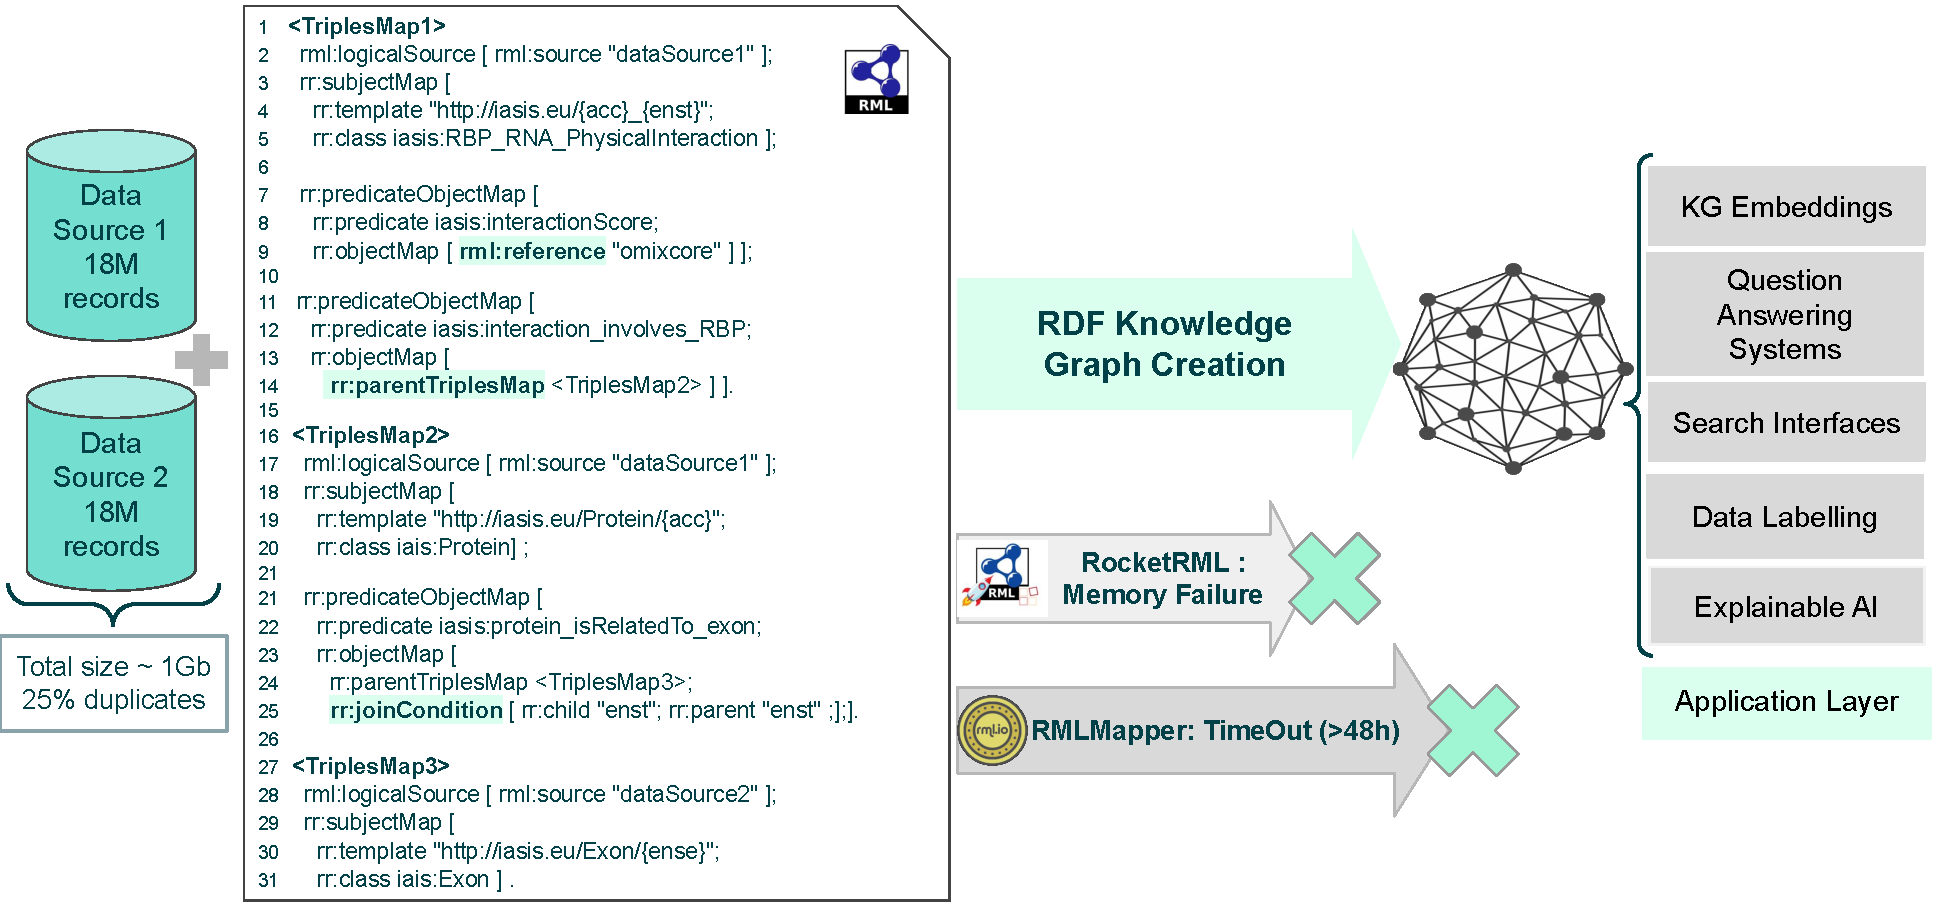
\includegraphics[width=0.7\textwidth]{figures/Motivating_Example_v1.1.pdf}
\caption[SDM-RDFizer motivating example]{\textbf{Motivating example.} Available RML engines, implementing naive join strategy, fail to create a KG from two biomedical datasets with a total size of 1GB and 25\% duplicates.} 
\label{fig:motivatingExample}
\end{figure}
\textbf{Our Resource:} We address the problem of efficient knowledge graph creation, and propose a resource named SDM-RDFizer which is able to transform data from myriad data sources into an RDF knowledge graph. SDM-RDFizer implements a set of unique physical operators and data structures that speed up the execution of the mapping rules that specify a knowledge graph creation process. The current version of SDM-RDFizer is customized for RML, a mapping language extensively used for the creation of knowledge graphs in diverse domains~\citep{dimou2014rml}.    
SDM-RDFizer is publicly available as a resource in a Github\footnote{\url{https://github.com/SDM-TIB/SDM-RDFizer}} and in Zenodo\footnote{\url{https://doi.org/10.5281/zenodo.3872103}}. SDM-RDFizer is used in more than eight international projects. Moreover, experimental results reveal the contribution that SDM-RDFizer makes to the repertoire of efficient technologies for knowledge graph management.  
\begin{figure}[t!]
    \centering
    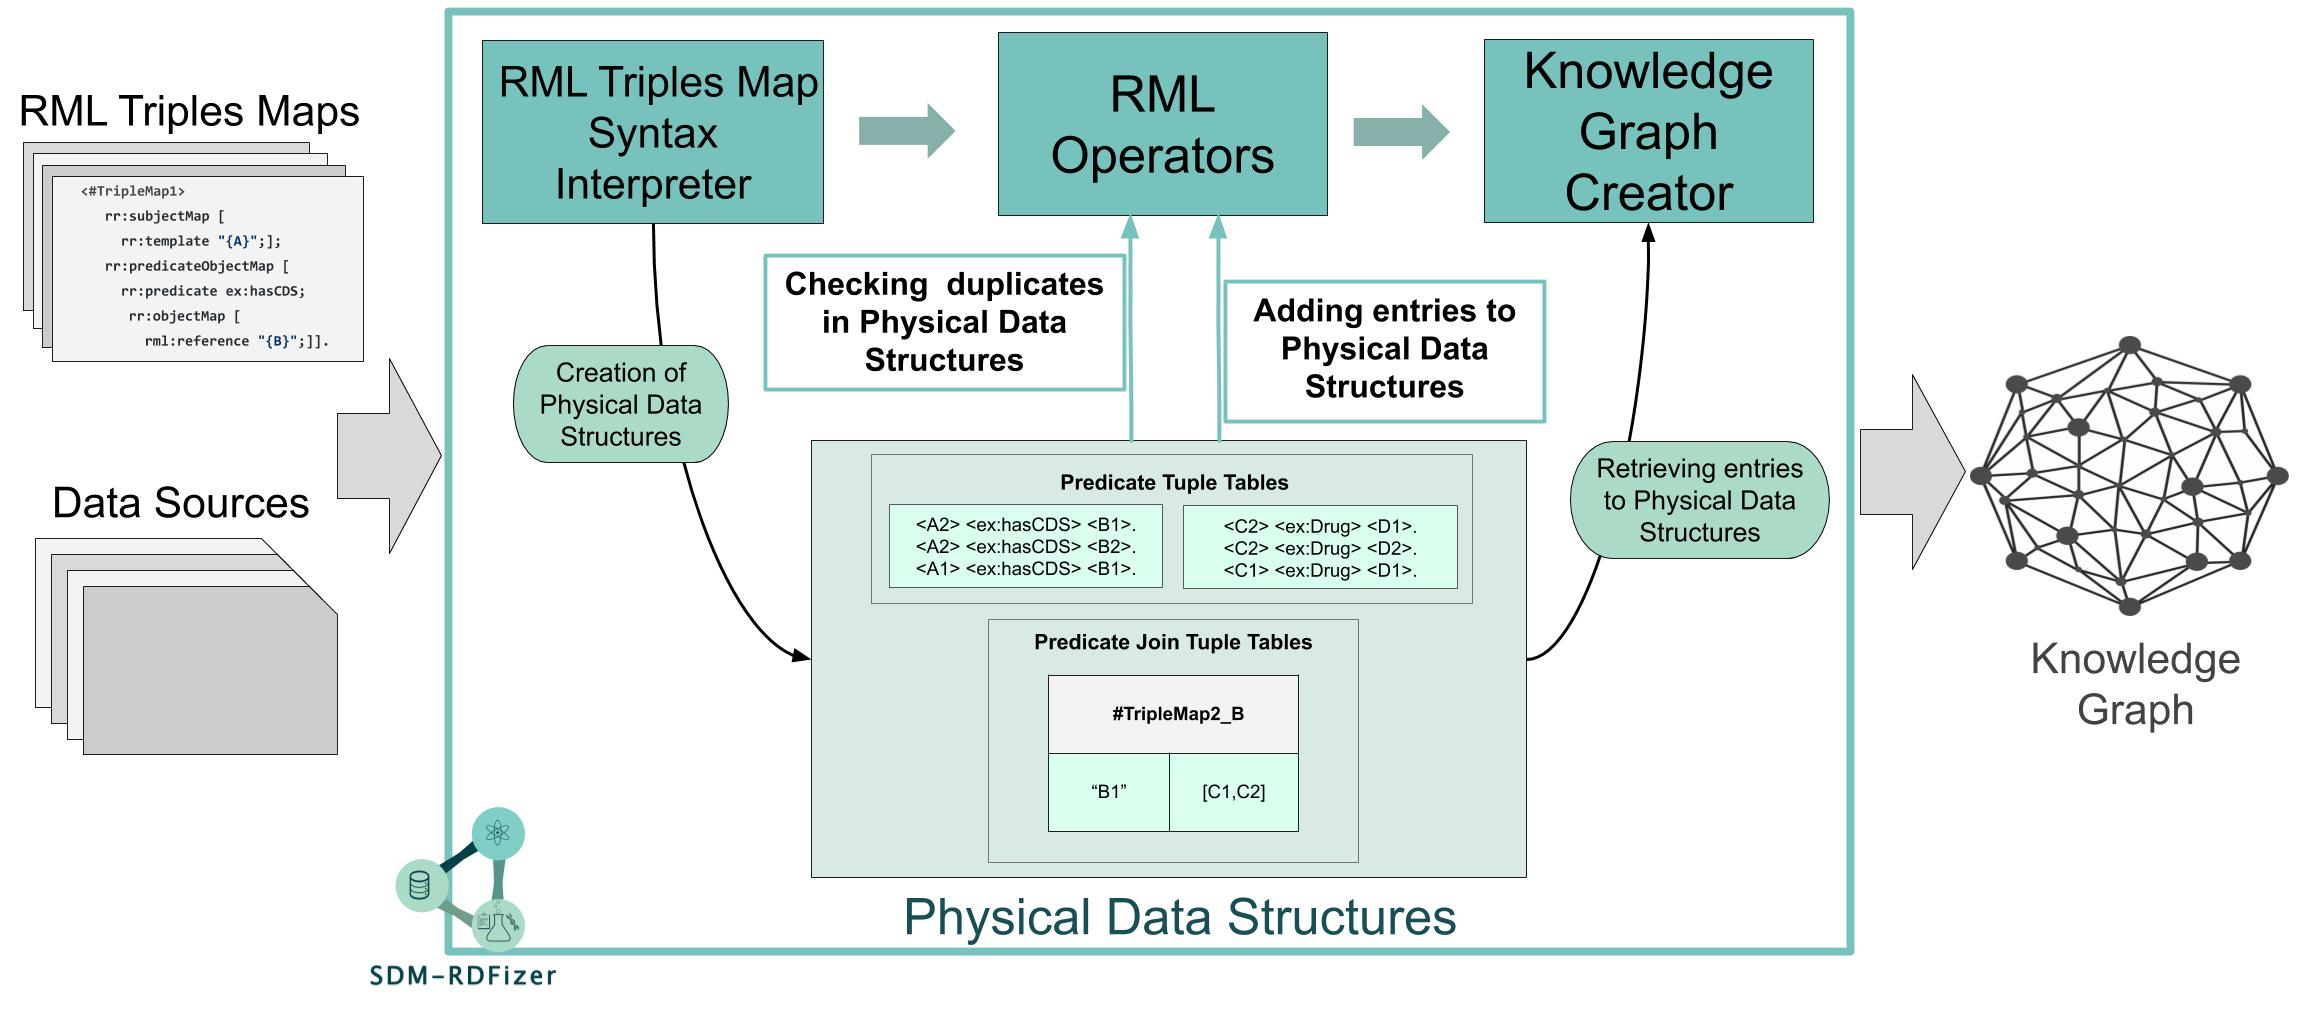
\includegraphics[width=1\textwidth]{figures/architecture_v1.1.jpg}
    \caption[SDM-RDFizer architecture]{The architecture of the SDM-RDFizer.}
    \label{fig:architecture}

\end{figure}



\begin{figure}[h!]
 \centering
 \subfloat[Predicate Tuple Table]{
      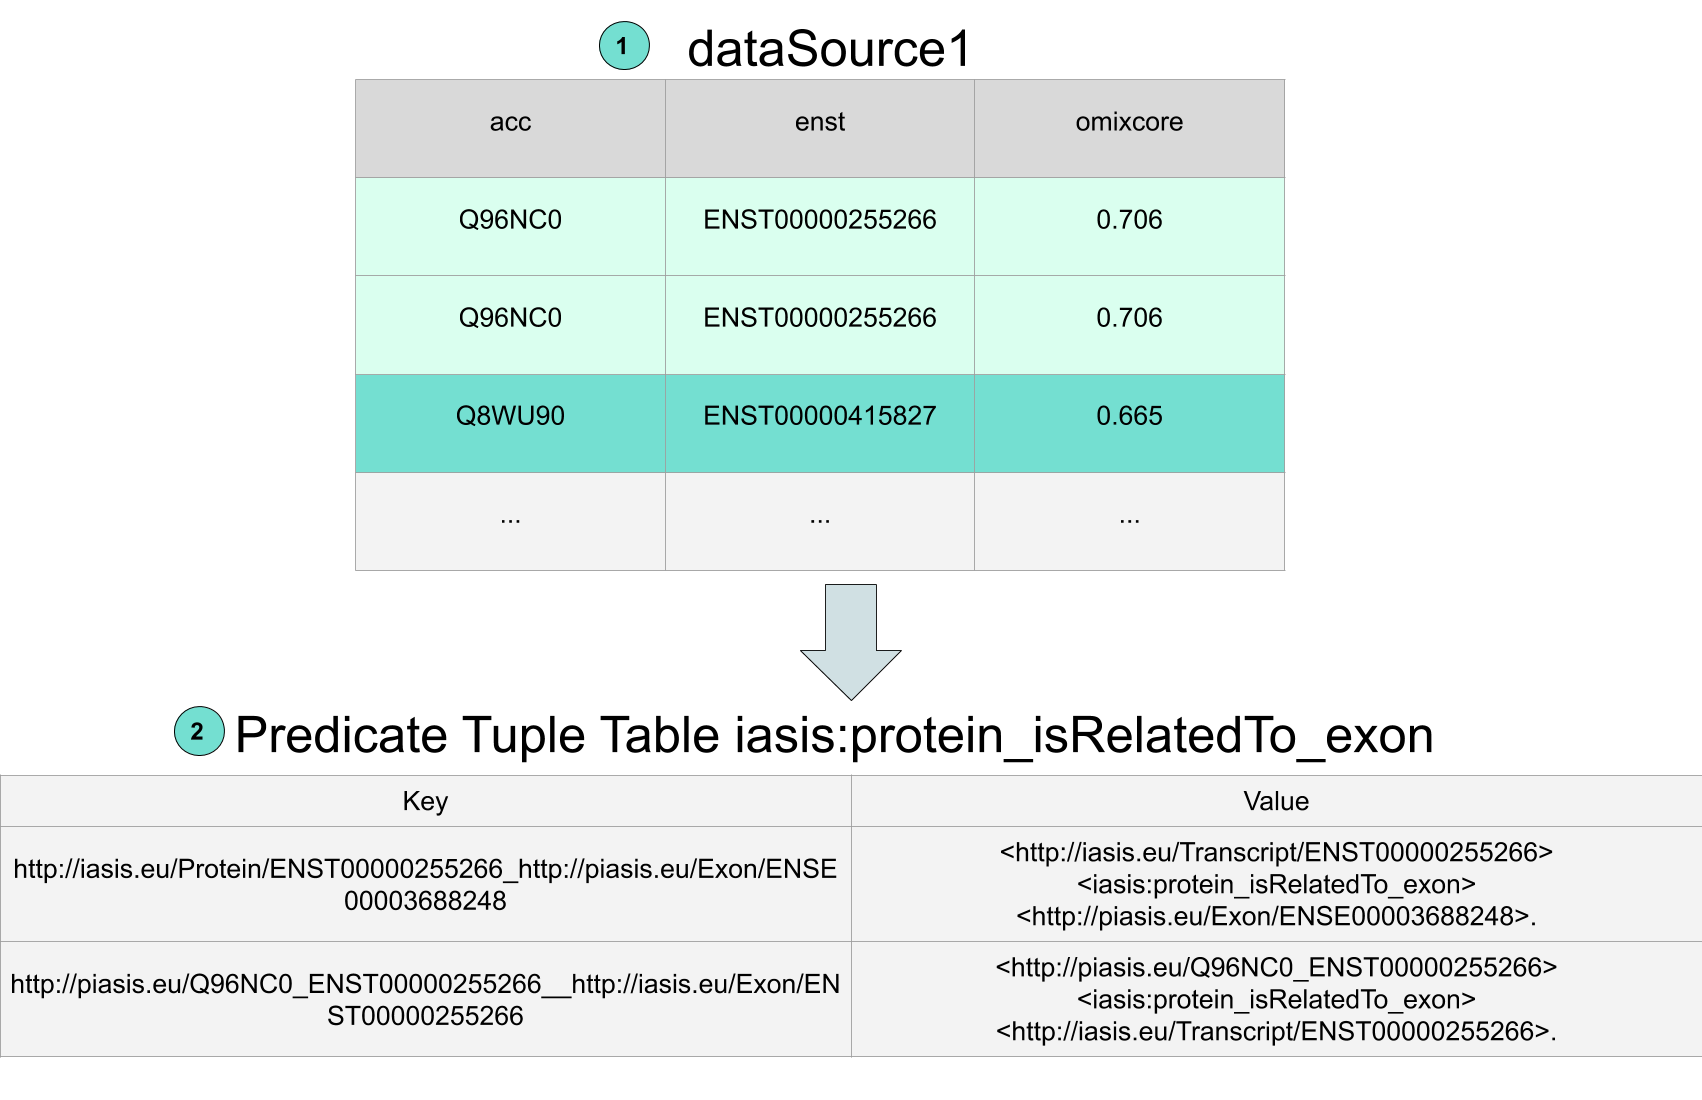
\includegraphics[width=0.8\textwidth]{figures/PTT.png}
    \label{fig:ptt}}

  \subfloat[Predicate Join Tuple Table]{
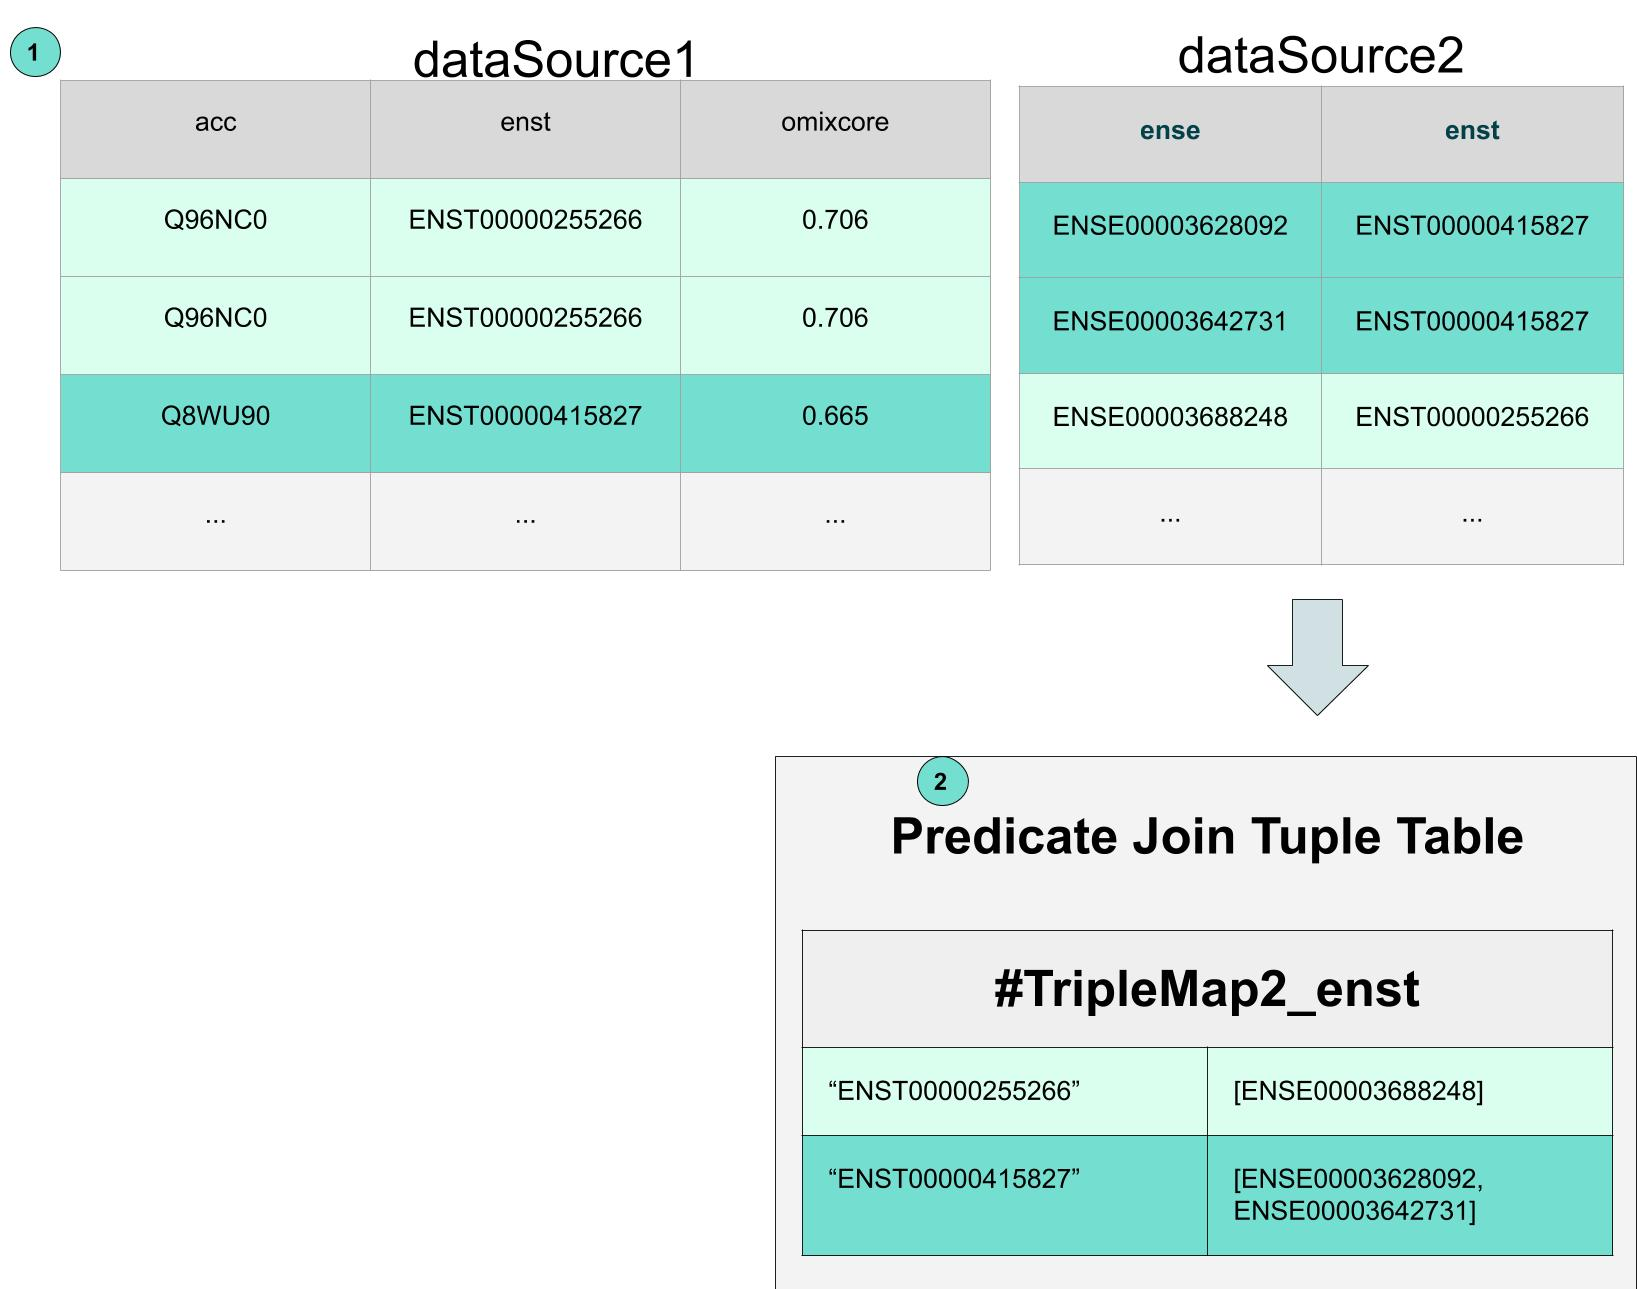
\includegraphics[width=0.8\textwidth]{figures/PJTT.jpg}
    \label{fig:pjtt}}
    \caption[Physical Data Structures for KGC]{{\bf The Physical Data Structures.} The two physical data structures used by SDM-RDFizer are illustrated. (a) A Predicate Tuple Table with three entries. (b) A Predicate Join Tuple Table with two entries.}
    \label{fig:hash_table}
\end{figure}
\subsection{The SDM-RDFizer: An RML Engine}

This section describes the SDM-RDFizer in terms of its architecture, the physical operators that make up the execution engine of RML triples maps, and the main properties of these operators.  

\subsubsection{The SDM-RDFizer Architecture}
A data integration system \textit{DI} provides an abstract representation $\langle O,S,M\rangle$ to specify the mapping rules in a set $M$ that define the integration of a set $S$ of data sources into instances of a unified schema or ontology $O$. 
SDM-RDFizer receives as input a data integration system \textit{DI} and produces as output instances of the concepts in $O$ that result from the execution of the mapping rules in $M$ over the data sources in $S$. 
The current version of SDM-RDFizer is customized for interpreting data integration systems where mapping rules are specified in RML, and the output corresponds to an RDF knowledge graph with the ontology $O$. 
However, the SDM-RDFizer architecture can be easily implemented for other RDF based mapping languages (e.g., R2RML~\citep{R2RML}).  
The execution of the RML triples maps requires the interpretation of triples maps, the creation of physical data structures to store the results of the execution of the RML rules, and the generation of the knowledge graph from the results stored in the data structures. \autoref{fig:architecture} depicts SDM-RDFizer in terms of four main components that implement these steps. 

\noindent\textbf{RML Triples Map Syntax Interpreter:} translates the RML triples maps into the physical data structures that SDM-RDFizer uses to execute the RML triples maps and generate the RDF triples.

\noindent\textbf{RML Operators:} execute the interpreted triples maps over the respective data sources to generate RDF triples. 
During the execution of these operators, the physical data structures are accessed to check if an RDF triple has already been created.
If so, the generation of a duplicated RDF triple is avoided, otherwise, the triple is stored in the physical data structure.
SDM-RDFizer has three operators; they are explained in more detail in \autoref{operators}.
    \begin{itemize}
        \item \textit{Simple Object Map}: is the most basic of the operators to evaluate a \textit{simple predicate object map} statement in an RML triples map. The values of the \textit{object values} are collected from an attribute in the triples map source or are a constant. In the motivating example, this operator generates RDF triples according to the predicate object map in lines 7-9 in \autoref{fig:motivatingExample}.  
        \item \textit{Object Reference Map}: this operator \textit{references a second triples map}. The object of the first triples map is the subject of the second triples map. The main condition for this operator to work is that both triples maps have the same data source. An application of this operator in the motivating example can be seen in lines 11-14. 
        \item \textit{Object Join Map}: this operator executes a \textit{join condition} between two RML triples maps with different data sources. In the motivating example, this operator is utilized to execute the predicate object map in lines 21-25 in \autoref{fig:motivatingExample}.
    \end{itemize}
    
\noindent\textbf{Physical Data Structures:} store results generated so far and avoid the generation of duplicates during the execution of RML triples maps. They are of two types: 
\begin{itemize}
\item i) Predicate Tuple Table (PTT): to store per each of predicate $p$ in at least one triple map, the RDF triples generated for $p$ so far. 
\item ii) Predicate Join Tuple Table (PJTT): to store the values of the subjects generated by a triples map that are associated with the values that meet a join condition in the triples map.  
\end{itemize}
These structures are explained in more detail in \autoref{pds}.

\noindent\textbf{Knowledge Graph Creator:} collects RDF triples stored in PTTs and adds them to the output knowledge graph. The knowledge graph creation is performed incrementally, i.e., as soon as a new RDF triple is added into a PTT, the RDF triple is also included in the knowledge graph. To avoid the same RDF triple to be added more than once, the knowledge graph creator maintains per PTT $t$, the timestamp of the last RDF triple that was selected from $t$. 

\subsubsection{Physical Data Structures}
The SDM-RDFizer utilizes two physical data structures as a means to optimize the creation of knowledge graphs. These data structures help with the removal of duplicates and to avoid unnecessary operations, like uploading the parent triples map's data source of a join multiple times. In the following subsection, the physical data structures used by SDM-RDFizer are described. 
\label{pds}

\noindent\textbf{Predicate Tuple Table (PTT)} 
For each predicate $p$ defined in an object triples map, a PTT is created to store the RDF triples generated so far. Physically, PTTs are implemented as hash tables where the hash key of an entry corresponds to an encoding of the subject and object of a generated RDF triple, and the value of the entry corresponds to the RDF triple. The main use of this table is to avoid the duplicate generation of an RDF triple. 
If a generated RDF triple is present within PTT, that means that the triple has been previously generated, and it needs to be discarded. But if the generated RDF triple is not present within PTT, then it is new and must be added to PTT and to the knowledge graph. As it can be seen in the figure\autoref{fig:ptt}, the data source is transformed into RDF triples which checked in the corresponding PTT. As RDF triples of a predicate $p$ can be generated from the execution of different triples maps, PTTs bring great savings not only in sources with high-duplicated rates but also when data sources that generate RDF triples of $p$ also overlap.  

\noindent
\noindent\textbf{Predicate Join Tuple Table (PJTT)}
A PJTT stores the values generated during the execution of a join condition between two RML triple maps, e.g., lines 21-25 in \autoref{fig:motivatingExample}, the predicate object map is defined in terms of a join of triples map \texttt{TriplesMap1} (child map) to \texttt{TriplesMap2} (parent map). For each RML triples map $M_i$ that is referred as a parent triples map in a join condition $B$, a predicate join tuple table $M_i \_B$ is created, e.g., \texttt{TriplesMap2\_enst} in our running example. 
Physically, predicate join tuples are hash tables. The hash key of an entry corresponds to the encoding of each of the values of the attributes in the condition $B$ (e.g., \texttt{enst}), while the value of the entry is a set with all the subject values generated by $M_i$ (e.g., values of the subject of \texttt{TriplesMap2}) that are associated with the values of the attributes in $B$ represented in the entry hash key.  
 Additionally, a PJTT enables direct access to the subjects associated with the join condition $B$, allowing thus for the join implementation as an index join.  
 In the example shown in Figure\autoref{fig:pjtt}, "enst" is the join condition between the triples maps. The data is organized as the values of the join conditions with its respective value in dataSource2. For example, we have the value "ENST00000415827" and its associated values "ENSE00003628092" and "ENSE00003642731".  In PJTT, "ENST00000415827" is the key in the hash table and "ENSE00003628092" and "ENSE00003642731" are the values. Finally, to identify an entry in PJTT, a key is generated from the identifier of the parent triples map and the join condition.  
\begin{figure}[h!]
 \centering
 \subfloat[Simple Object Map]{
      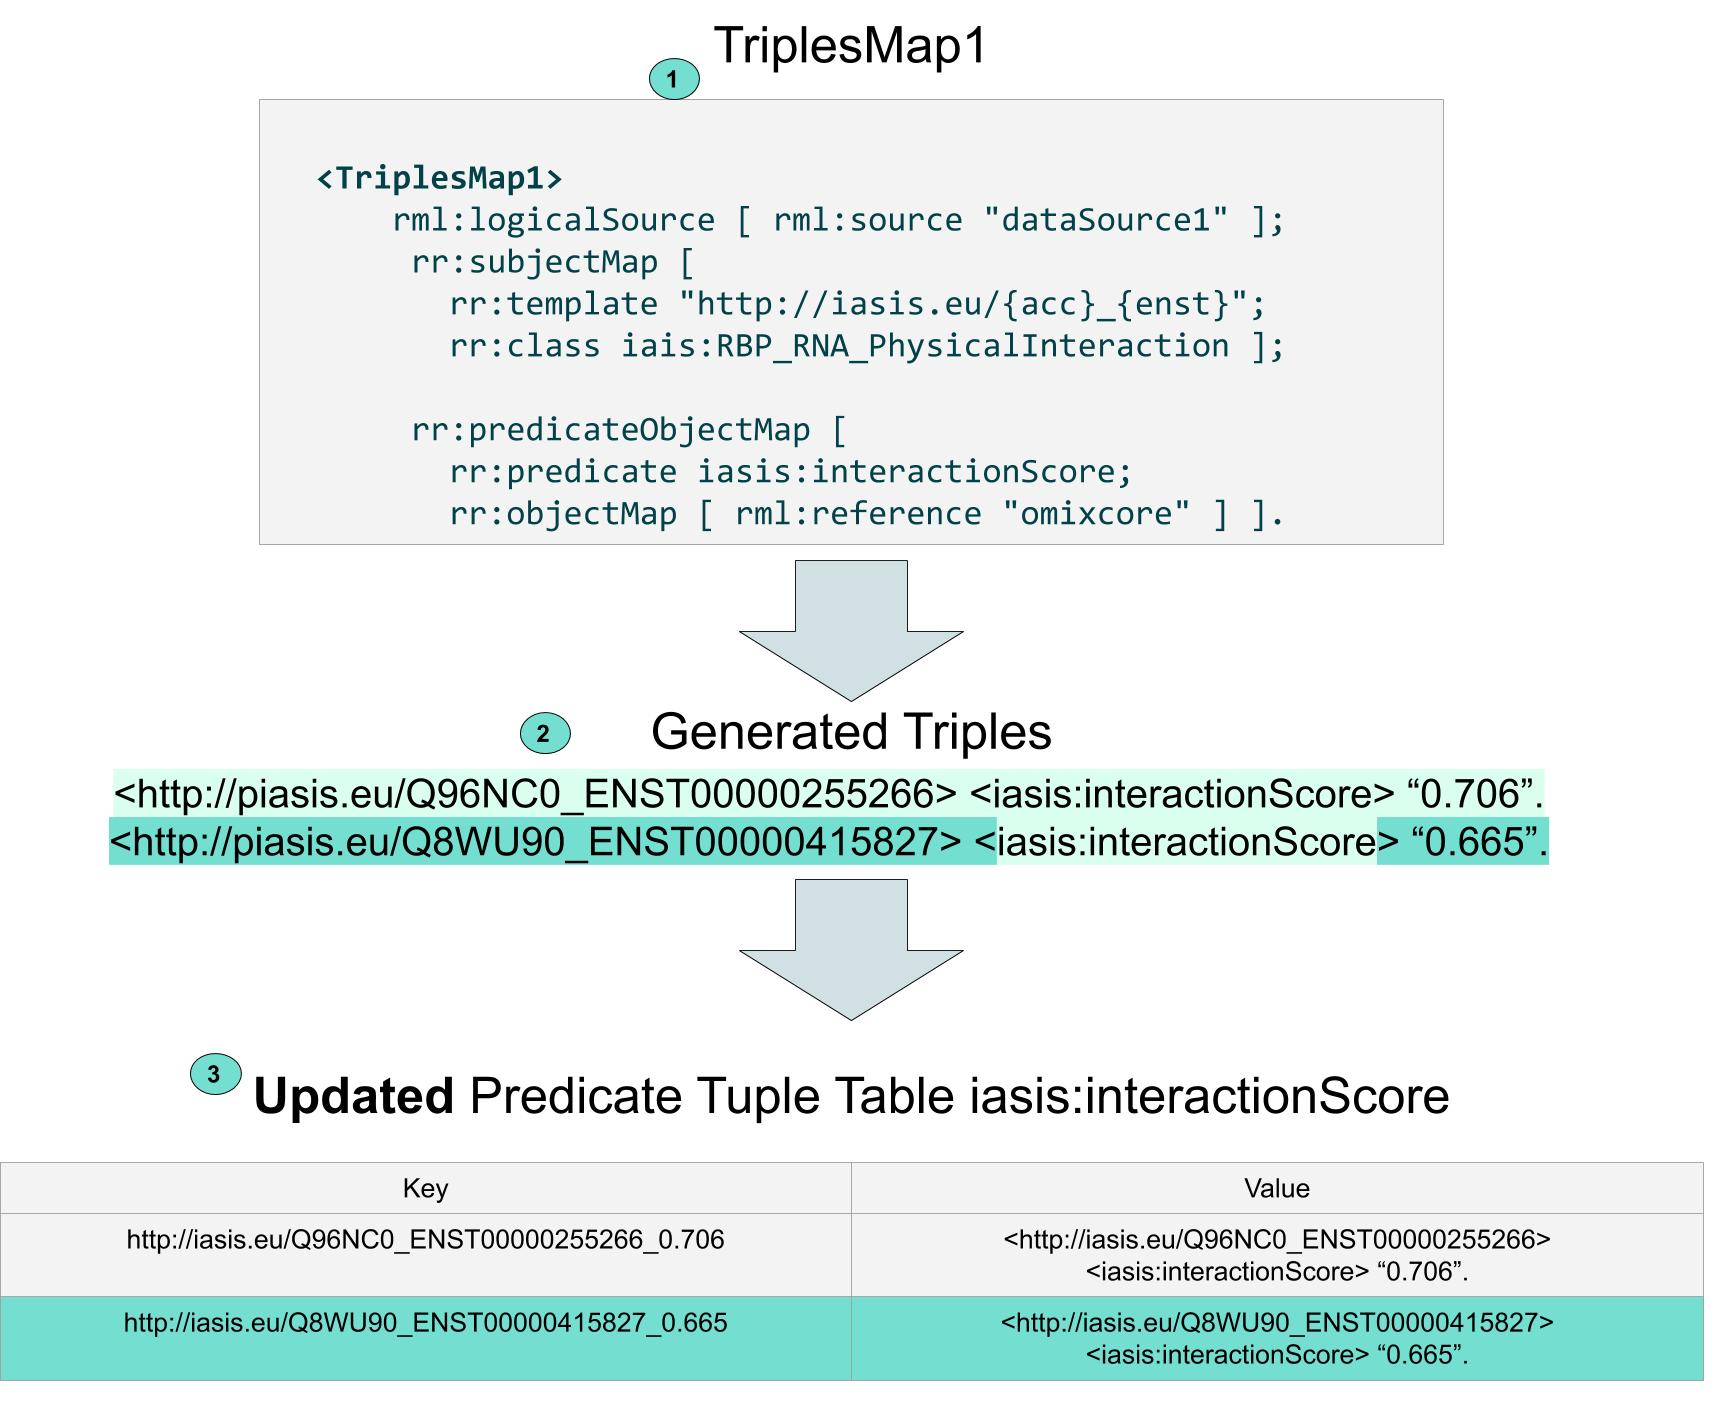
\includegraphics[width=0.45\textwidth]{figures/Basic_conversion_v1.1.jpg}
    \label{fig:om}}
  \subfloat[Object Reference Map]{
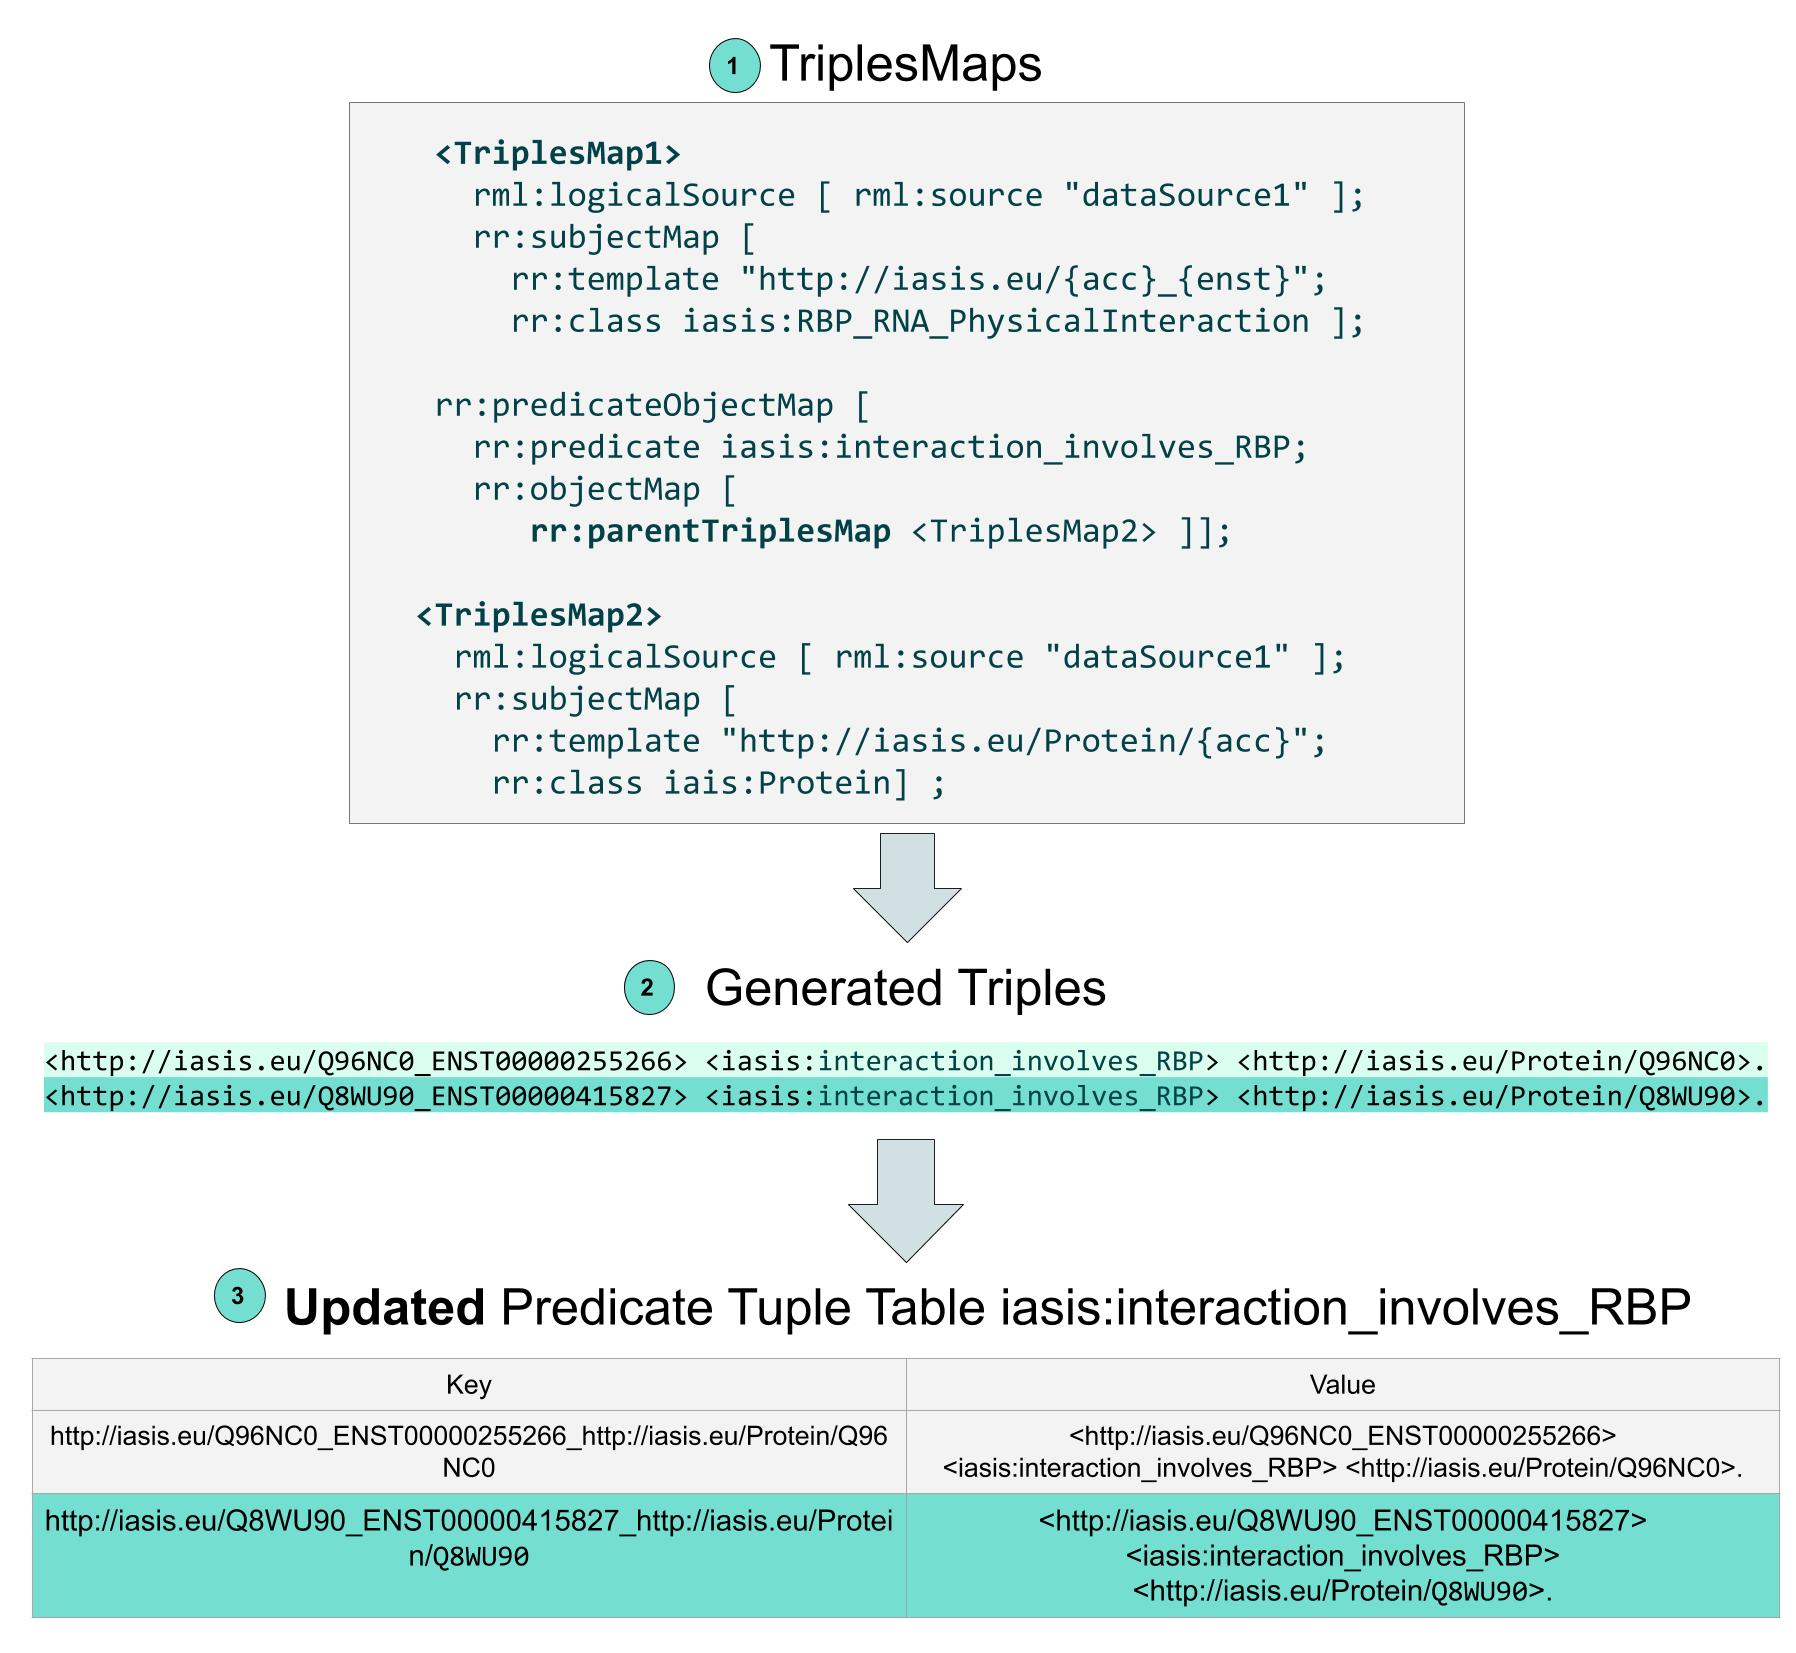
\includegraphics[width=0.45\textwidth]{figures/Mapping_reference_v1.1.jpg}
    \label{fig:orm}}

  \subfloat[Object Join Map]{
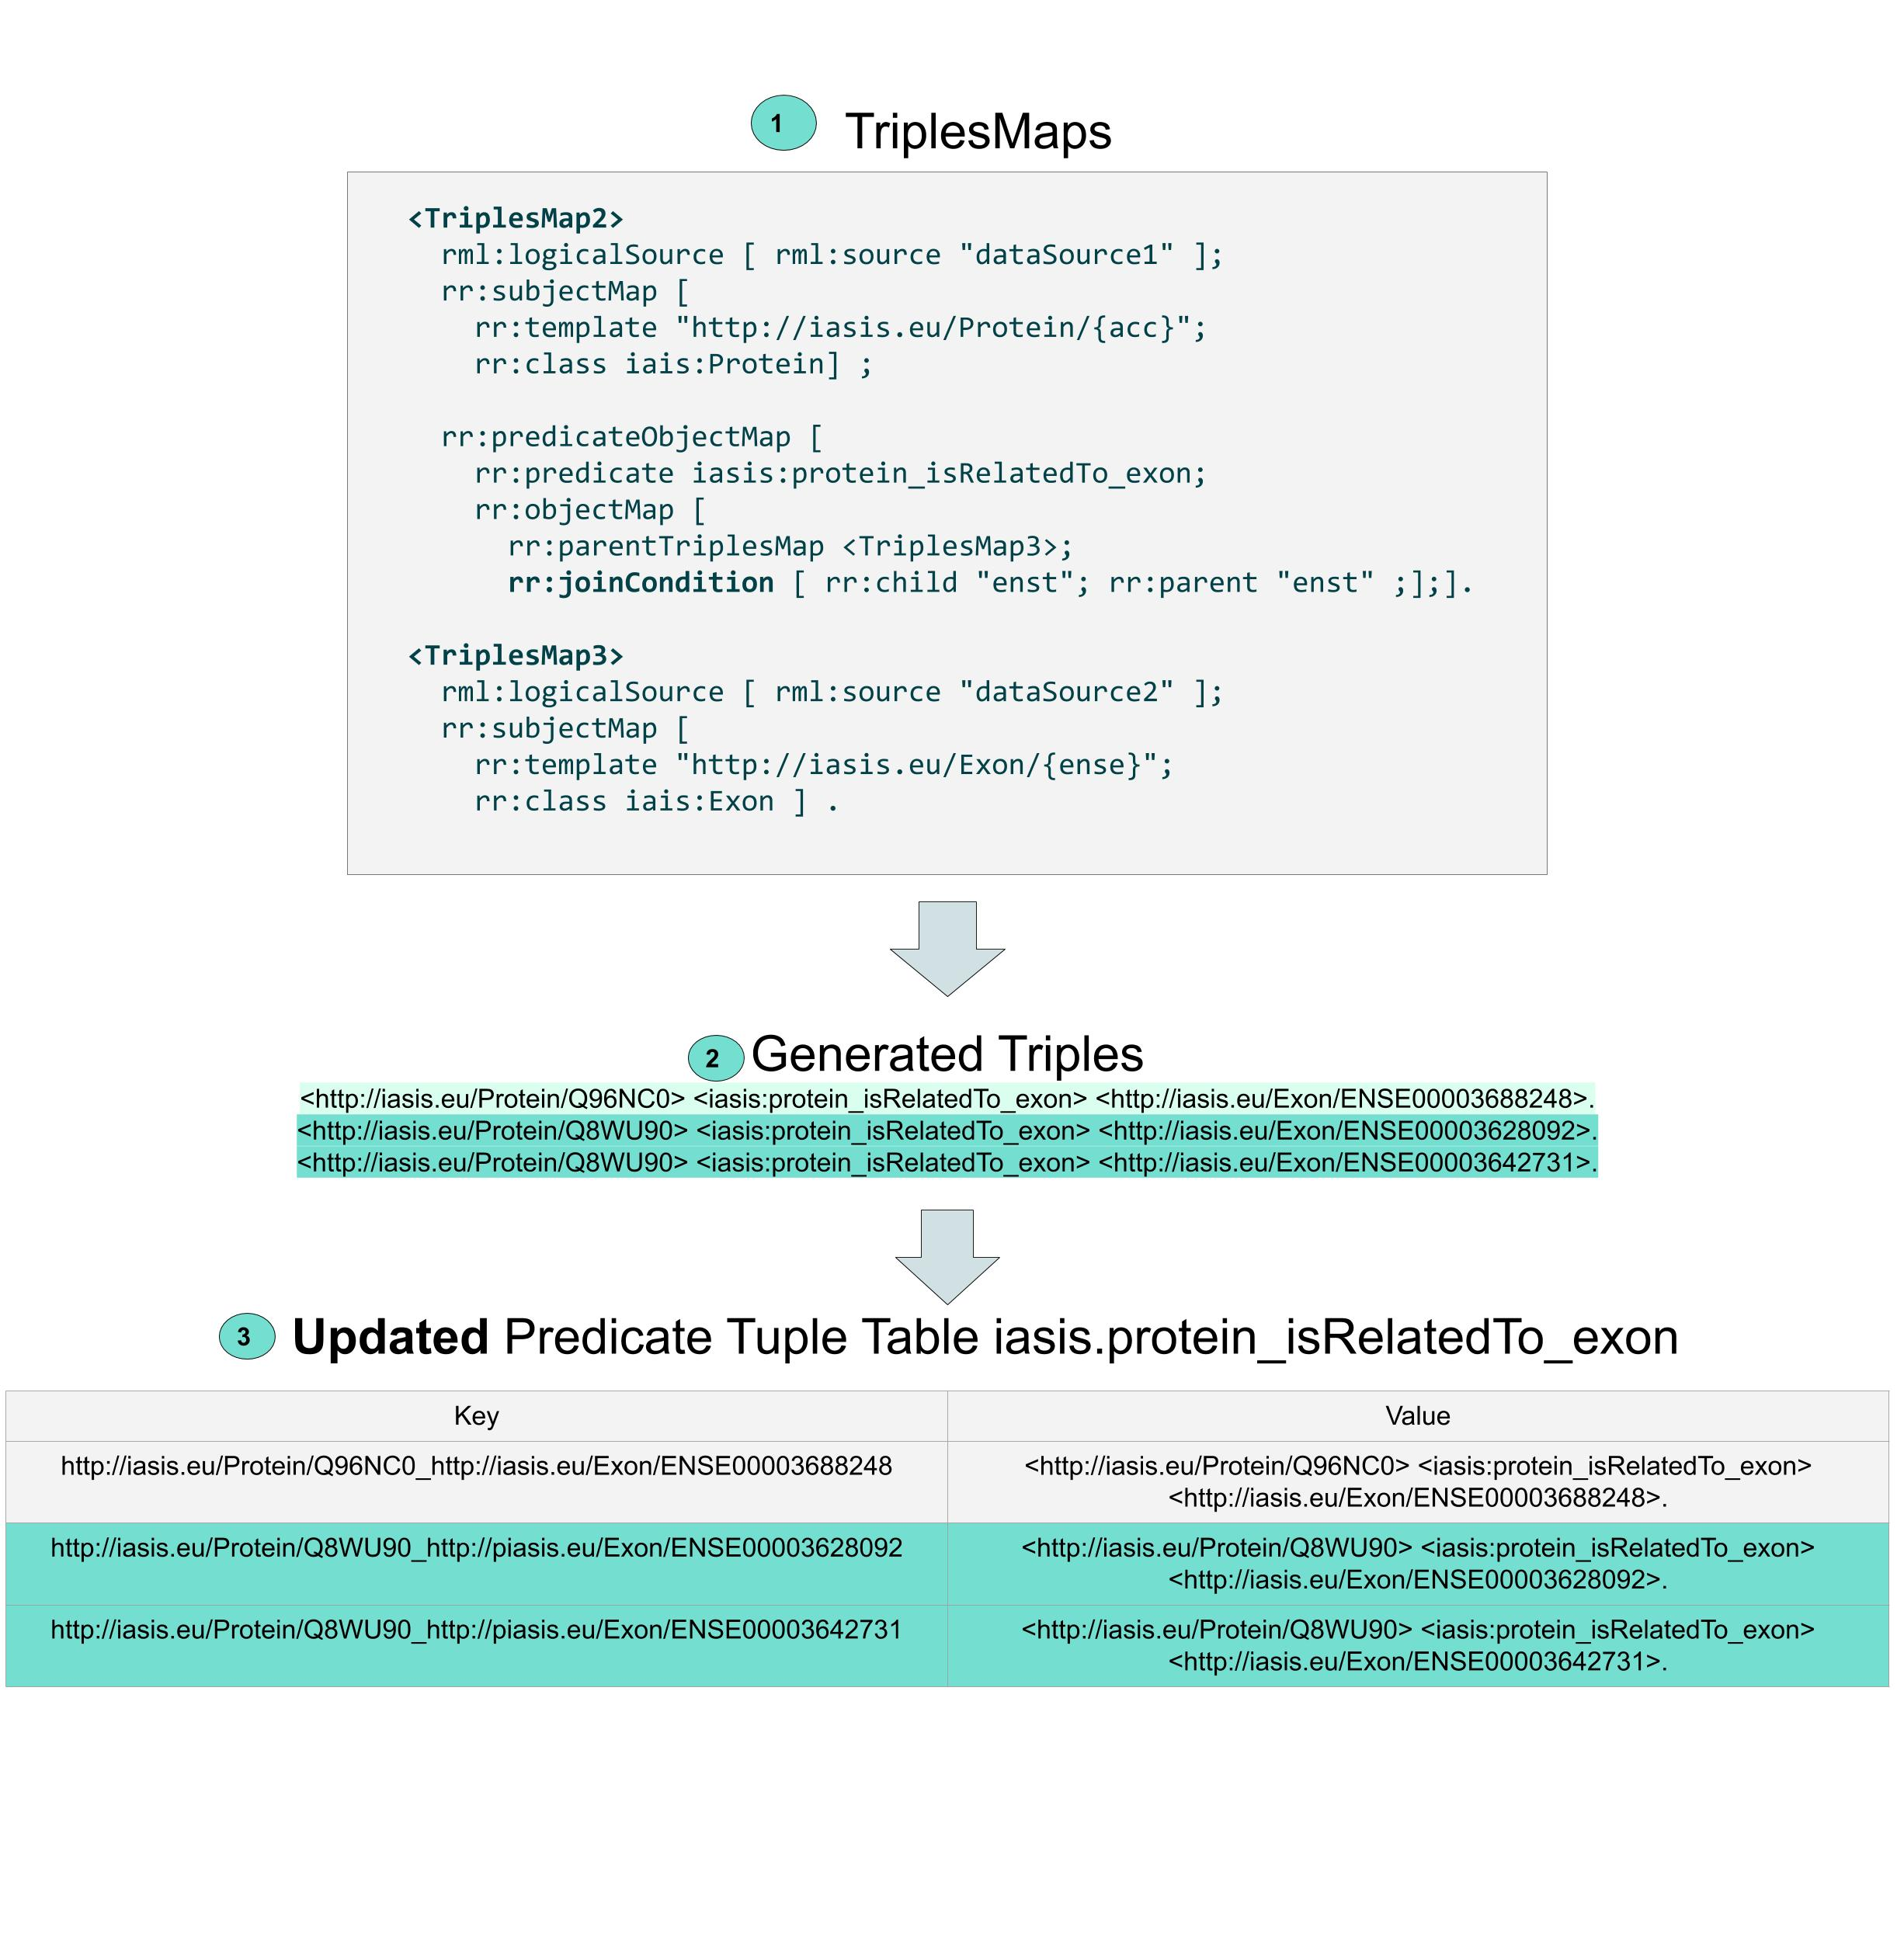
\includegraphics[width=0.6\textwidth]{figures/Join_v1.1.jpg}
    \label{fig:ojm}}
    \caption[Efficient Physical operator for KGC]{SDM-RDFizer implements three physical RML operators that rely on PTTs to avoid the generation of duplicates. Object Join Maps resort to PJTTs to provide a direct access to the inner tables (i.e., the parent triples maps) of a join between two triples maps; also, PJTTs avoid the traversal of a parent triples map in case it is referenced by more than one triples map.}
    \label{fig:DTR}
\end{figure}

\subsubsection{RML Operators and Algorithms}
\label{operators}
%Brief Overview
SDM-RDFizer implements three different operators for the creation of knowledge graphs. Depending on the type of the triples map, the SDM-RDFizer executes the respective operator. If the triples map has a join condition, then an \textbf{Object Join Map} operator is used. If the triples map have a reference to another triples map but do not have a join condition, then the \textbf{Object Reference Map} operator is used. Finally, if the triples map does not have a join condition or a reference to another triples map, then the \textbf{Simple Object Map} is used. We now describe the operators in more detail.

\noindent\textbf{Simple Object Map (SOM)}
 It is the most basic operator that SDM-RDFizer can execute and enables the generation of an RDF triple by executing a simple predicate object map statement. As it is illustrated in Figure\autoref{fig:om}, given a triples map and its respective data source, SDM-RDFizer generates RDF triples following what is established in the map. Each generated RDF triple is checked against the corresponding predicate tuple table (\textbf{PTT}). If the generated RDF triple already exists in PTT, then it is discarded. In the opposite case, the RDF triple is added both to PTT and to the knowledge graph. This operation is depicted in Figure\autoref{fig:om} where two RDF triples are generated. "<http://iasis.eu/Q8WU90\_ENST00000415827> <iasis:interactionScore> “0.665”." is not in PTT, then, it is added both to the table and to the knowledge graph.  

\noindent\textbf{Object Reference Map (ORM)}
It seeks to expand what is established in Simple Object Map. By using the subject of a triples map as the object of another triples map. The main condition for this operator to work is that both triples maps have the same data source. Afterwards, the same process as in Simple Object Map is applied on the generated RDF triples, i.e., the triples are checked against PTT to determine if the triples are required for the knowledge graph creation. An example of this operation is in Figure\autoref{fig:orm}. In the figure, there are two triples maps, where the \textit{<TripleMap2>} acts as the parent triples map. Two RDF triples are generated but only the new one is included in the PTT. 

\noindent\textbf{Object Join Map (OJM)}
It seeks to expand what is established in Object Reference Map, but the main difference is that triples maps have different data sources. By using the corresponding PJTT, SDM-RDFizer implements an index join where the outer table of the join corresponds to the values in the child map, and the inner table to the PJTT. Thus, to validate the satisfaction of a join condition $B$, the value of $B$ is checked in PJTT and if an entry $e$ exists with that hash key, all the subjects in $e$ are used to generate the resulting RDF triples. Finally, similar to the last two operations, the generated RDF triples are checked against the corresponding PTT to validate duplication and decide if they are going to be included in the knowledge graph. A way to better understand this operation is to view Figure\autoref{fig:ojm}. In the figure, the join condition is the column "enst" in both data sources. A PJTT table is created from the data associated with the join condition as shown in Figure\autoref{fig:pjtt}. Three RDF triples are generated and only two are not duplicates (i.e., they are not in the PTT). This operation is similar to Object Reference Map, since the object of the triples is the subject of the parent triples map. 
\subsubsection{Properties} 
We present the main properties of the RML operators implemented by SDM-RDFizer. Per operator \texttt{o}, we seek to compare the number of operations done by SDM-RDFizer versus the ones done by a na\"ive implementation of \texttt{o}; we named these expressions $\phi_{\texttt{o}}(.)$ and $\widehat{\phi}_{\texttt{o}}(.)$, respectively. Without lost of generality, we just focus on main-memory operations per operator, i.e., comparisons and insertions in main-memory data structures. Consider a predicate $p$, a multiset $N_p$, and set $S_p$; $N_p$ includes all the RDF triples of $p$ while $S_p$ is the corresponding set of $N_p$. Consider $|N_p|$ and $|S_p|$ as the cardinality of $N_p$ and $S_p$, respectively. In presence of a high-duplicate rate of RDF triples of $p$, $|S_p|$ is much smaller than $|N_p|$ (i.e., $|S_p| \ll|N_p|$).
\begin{itemize}
    \item \textbf{Simple Object Map (SOM):}
    Let $M$ be an RML triples map with an object triples map that defines $p$, $\phi_{\texttt{o}}(M)$ and $\widehat{\phi}_{\texttt{o}}(M)$ are defined as follows.  
  The na\"ive implementation of the simple object map operator $o$ in $M$ generates all the duplicates and then, it needs to execute a duplicate elimination process to add the RDF triples to the knowledge graph. Suppose a merge sort algorithm is conducted to eliminate duplicates \citep{BittonD83}\footnote{$\Theta(.)$ corresponds to the asymptotic notation}, then the following number of operations are required: 
       \[\widehat{\phi}_{\texttt{o}}(M)=
        |N_{p}| + |S_{p}| + \Theta(N_{p}log(N_{p}))\]
       
Contrary, the SDM-RDFizer algorithm of a simple object map resorts to a PTT of $p$ and never generates duplicates. As a result, the number of operations is defined as follows:
       \[ \phi_{\texttt{o}}(M)=|N_{p}| + 2|S_{p}|\]
       
    \item \textbf{Object Reference Map (ORM):} 
    This operator requires to define $p$, a reference of $M$ to a parent triple map $M_i$ expressed over the same data source $s$ of $M$. That is, the operator corresponds to a self-join over $s$ with a natural join condition on the attribute(s) that corresponds to the subject of $M$. As in a natural join, the join condition is not required. Assume $\Theta(1)$ is the cost of accessing the value of the subject of $M_i$ when $M$ is executed, then the number of operations is the same as executing a simple object map, i.e., 
    \[\widehat{\phi}_{\texttt{o}}(M)=
        |N_{p}| + |S_{p}| + \Theta(N_{p}log(N_{p}))\]
    \[ \phi_{\texttt{o}}(M)=|N_{p}| + 2|S_{p}|\]    
    \item \textbf{Object Join Map (OJM):}
    An Object Join Map executes a join between the data source of a child triple map $M$ and the data source of a parent triple map $M_i$ on a join condition $B$. In this case, $|N_p|$ represents the number of RDF triples resulting of evaluating the join and $|S_p|$ the number of duplicate-free RDF triples in $N_p$. Further, assume $|N_{\textit{parent}}|$ and $|N_{\textit{child}}|$ are the number of rows in the parent and child maps, respectively, to check to validate the join condition. If the na\"ive approach follows a nested loop join \citep{SteinbrunnMK97}, then 
    \[\widehat{\phi}_{\texttt{o}}(M)= |N_{\textit{parent}}| \times |N_{\textit{child}}| +
        |N_{p}| + |S_{p}| + \Theta(N_{p}log(N_{p}))\]
 Contrary, SDM-RDFizer relies on the PJTT $M_i \_B$ (of size $N_{\textit{parent}}$\footnote{We assume that a PJTT creation costs $N_{\textit{parent}}$ main-memory operations.}) and the PTT of $p$ to implement an index join that produces duplicate-free RDF triples. Thus, both physical data structures enable an efficient implementation of OJM. As a result, the number of operations is as follows:
 \[\widehat{\phi}_{\texttt{o}}(M)= 2|N_{\textit{parent}}| + |N_{\textit{child}}| +
        |N_{p}| + 2|S_{p}|\]
\end{itemize}
\begin{figure}[!tb]
 \centering
    \subfloat[10k records]{
    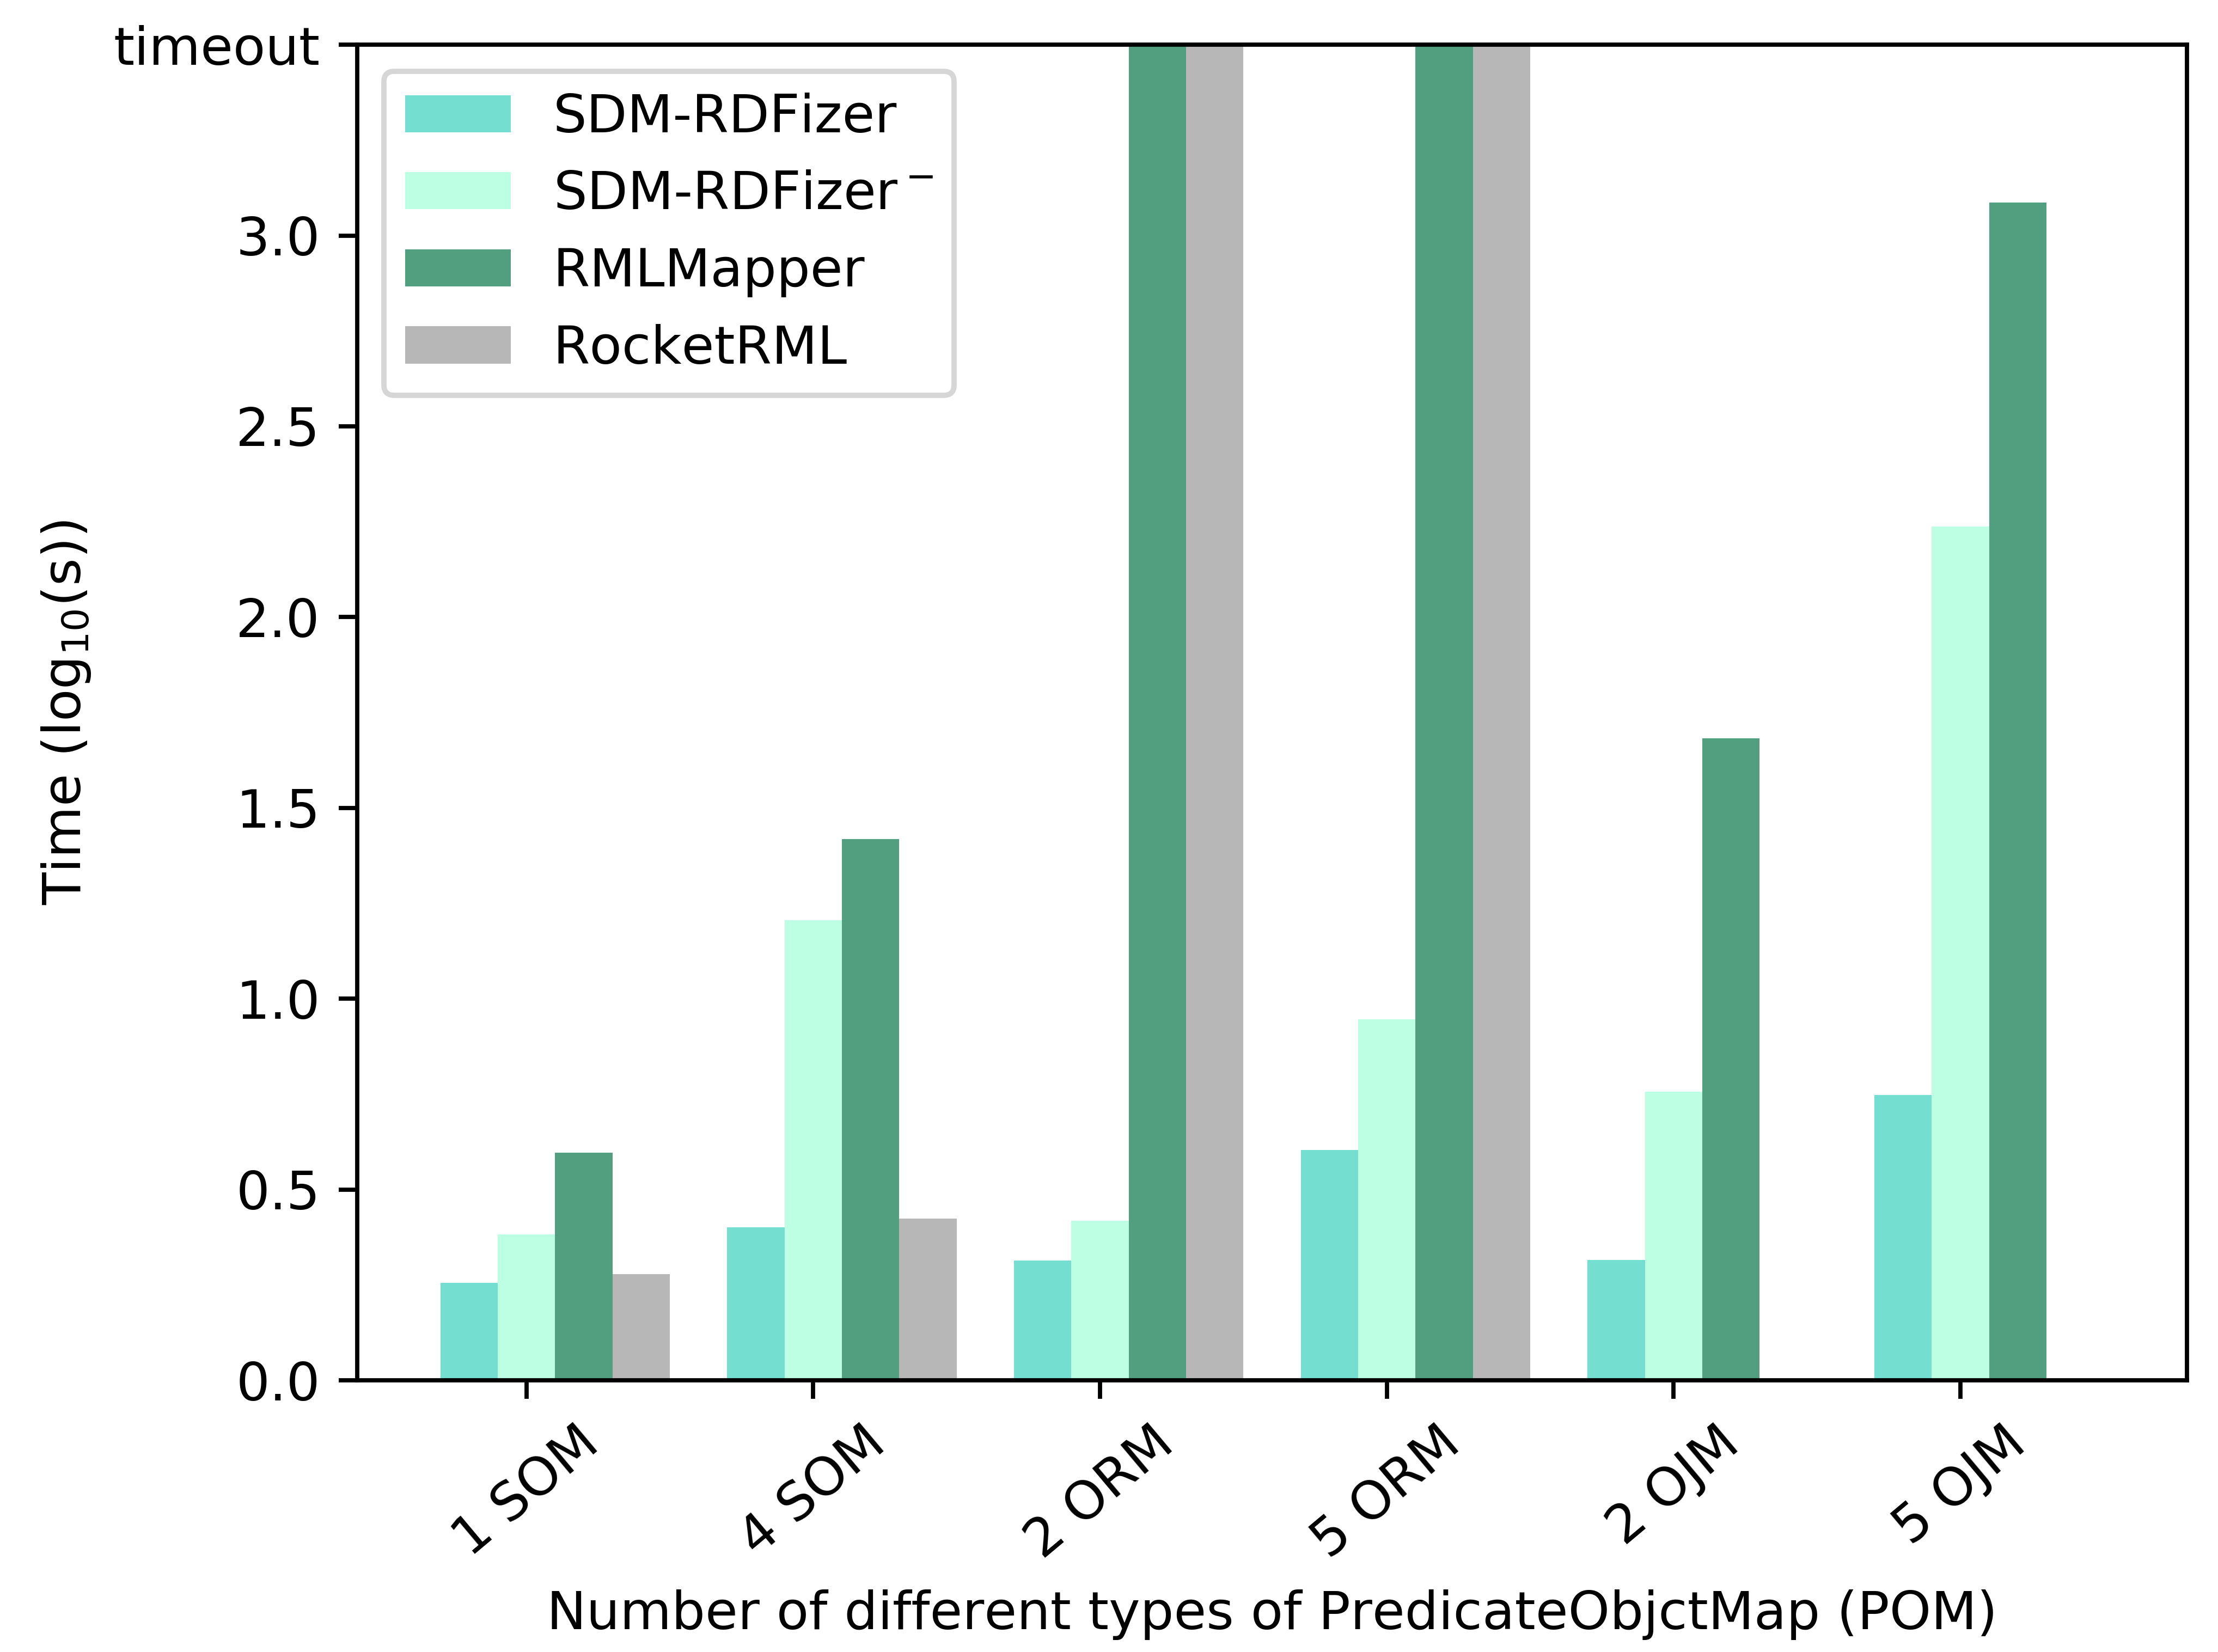
\includegraphics[width=0.45\columnwidth]{figures/sdmrdfizer/10k_vera25.png}
    \label{fig:vera25_10K}}
    \subfloat[100k records]{
    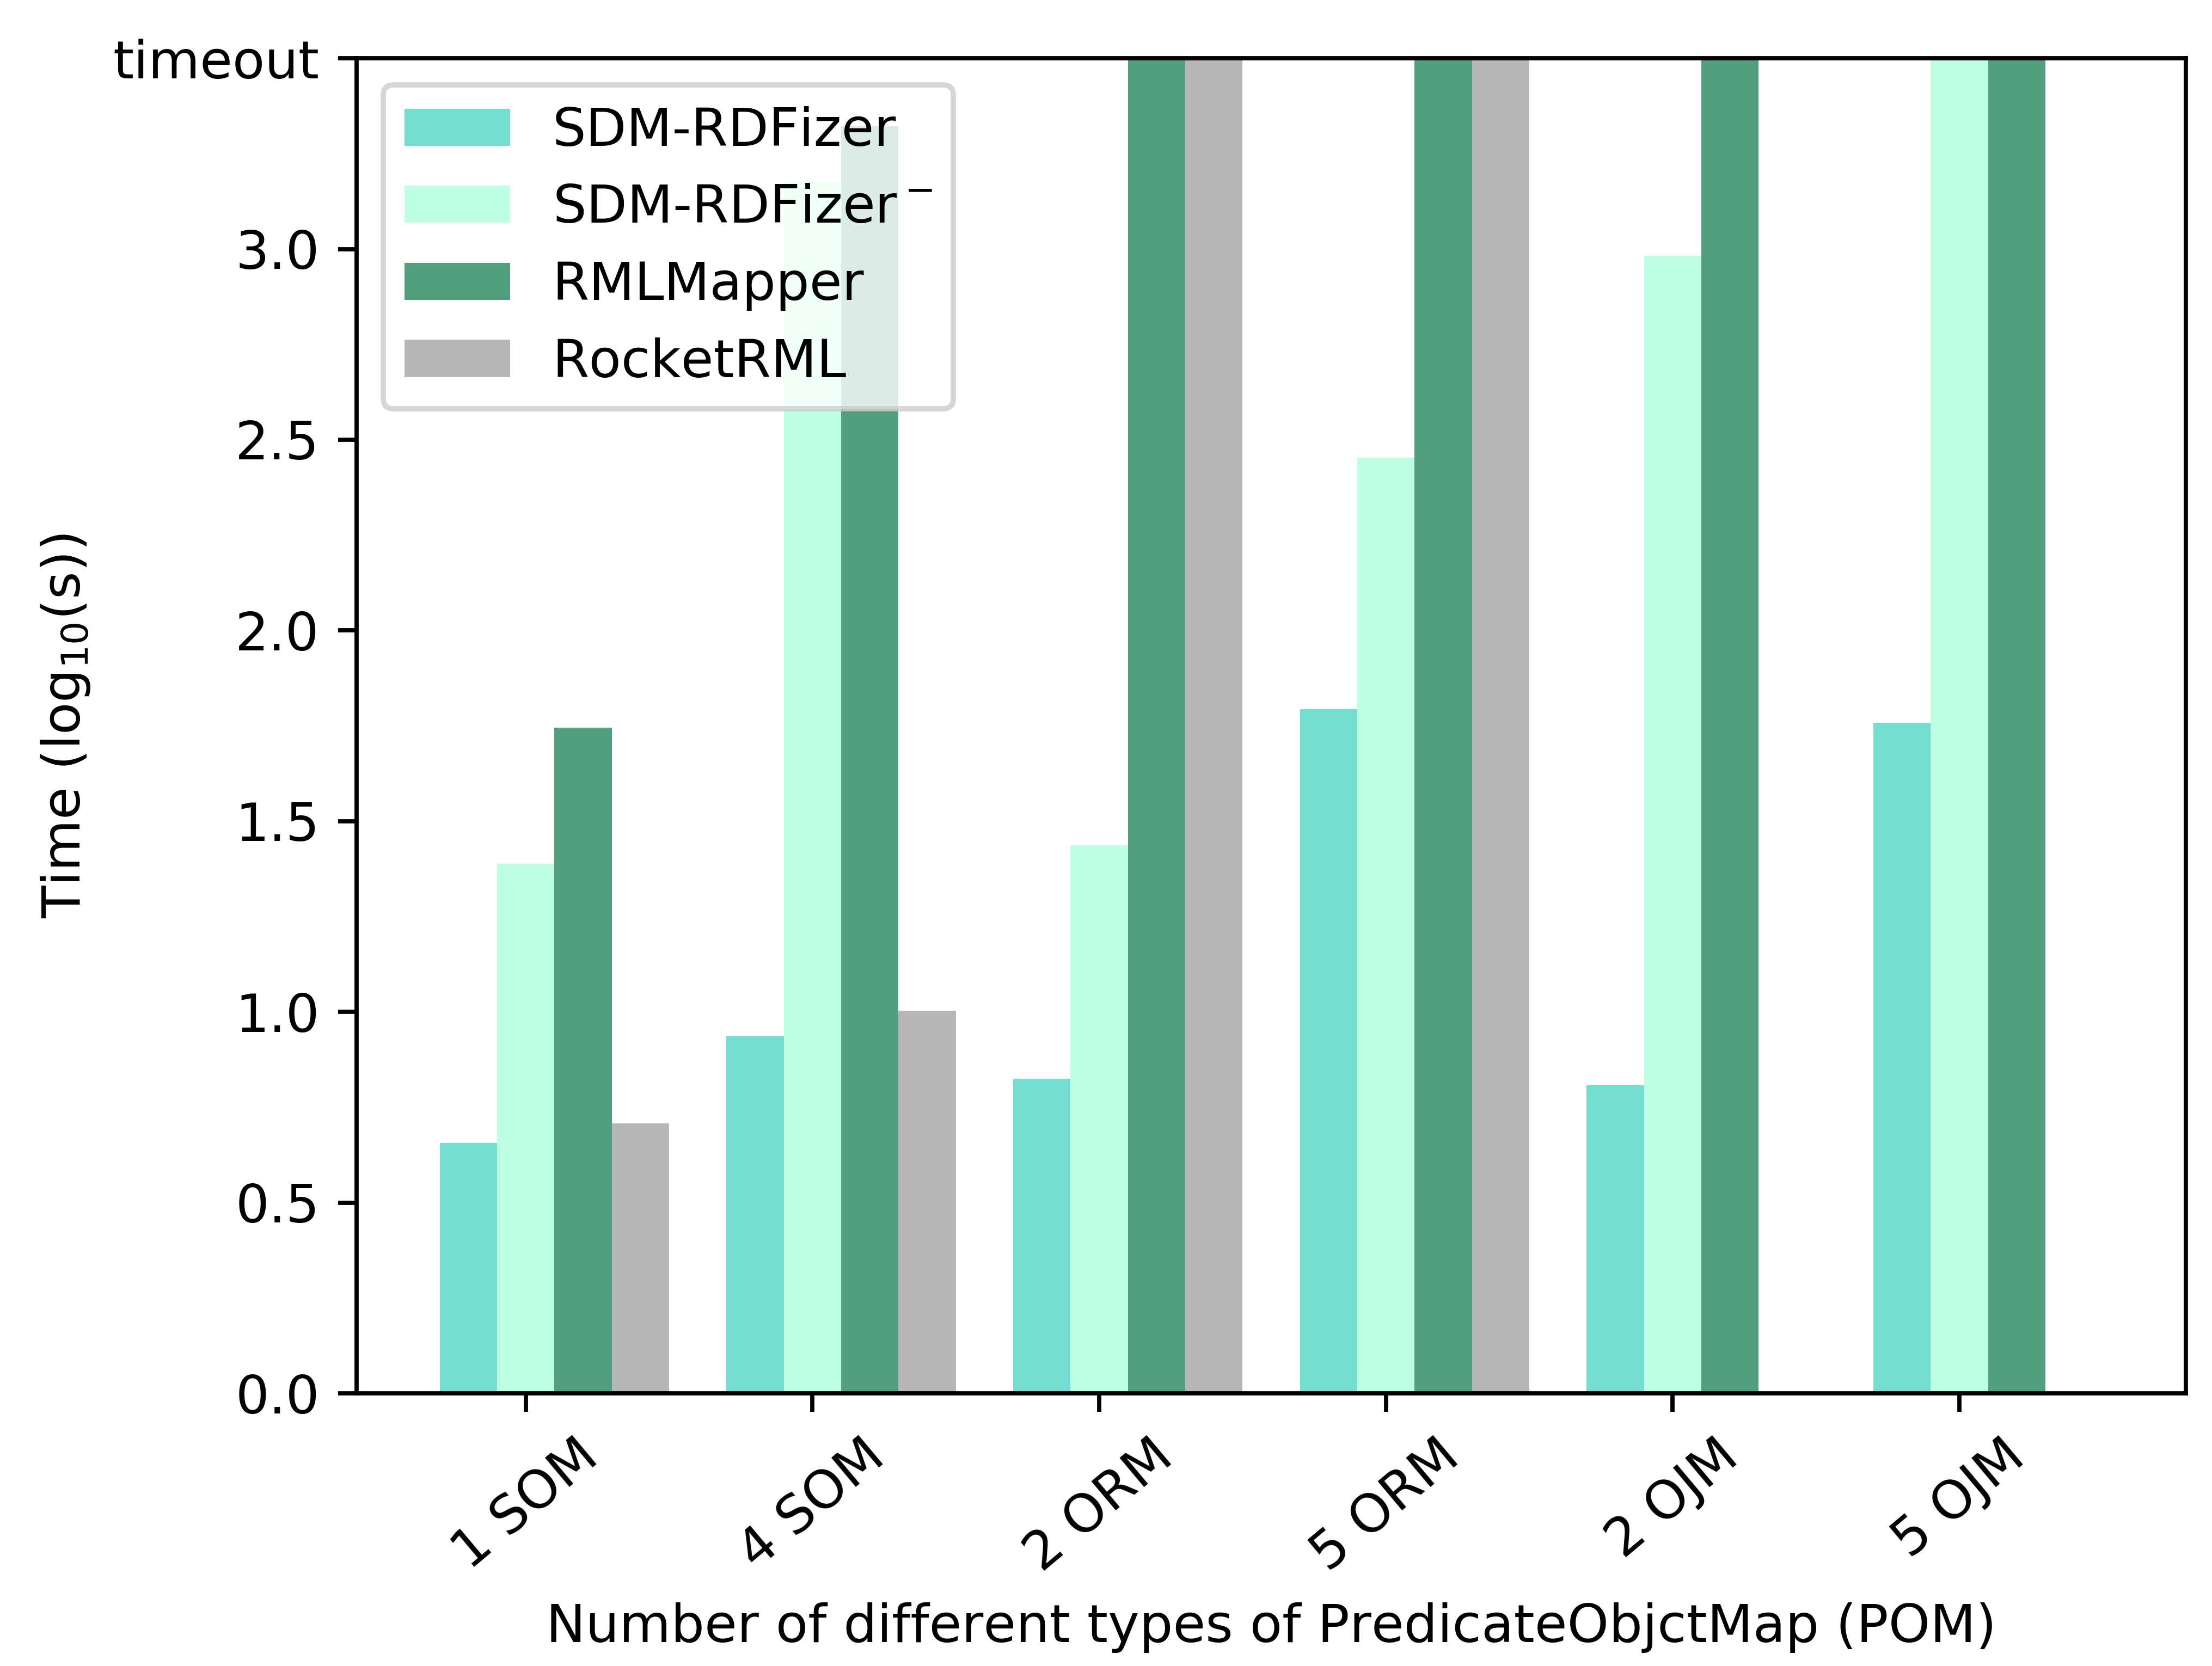
\includegraphics[width=0.45\columnwidth]{figures/sdmrdfizer/100k_vera25.png}
    \label{fig:vera25_100K}}
    \qquad
    \subfloat[1M records]{
    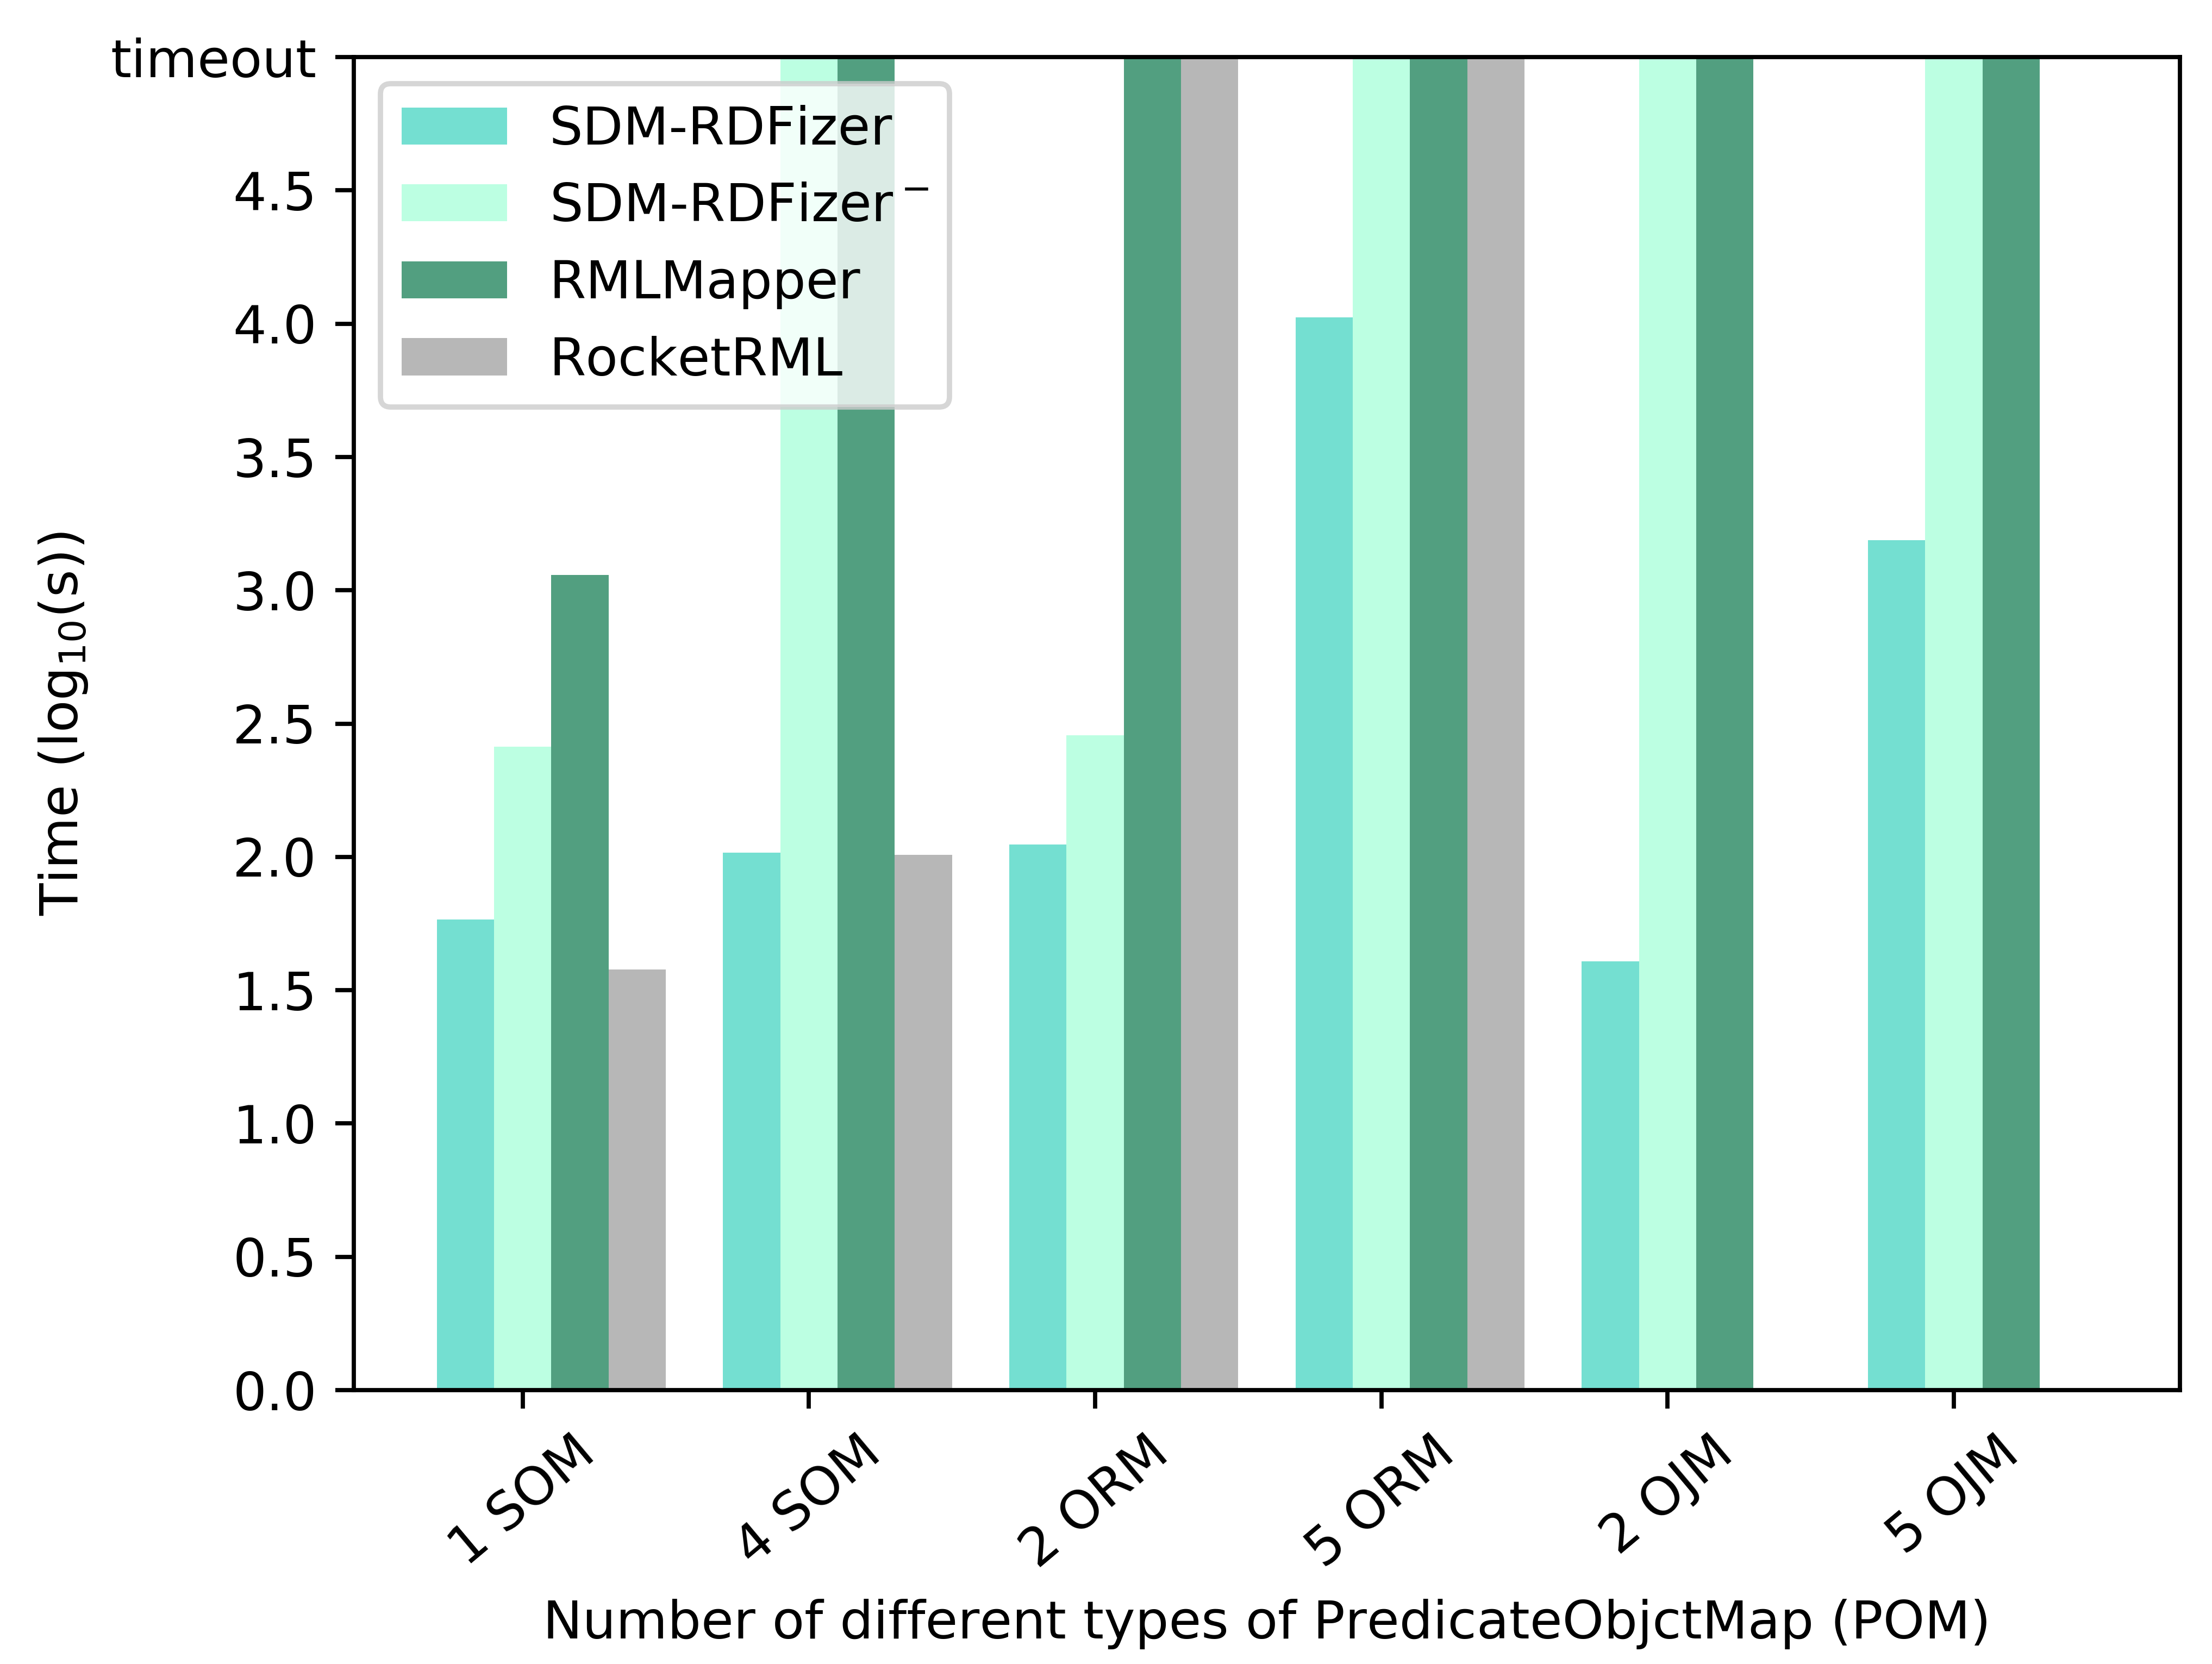
\includegraphics[width=0.45\columnwidth]{figures/sdmrdfizer/1M_vera25.png}
    \label{fig:vera25_1M}}
\caption[Execution time for with 25\% duplicates]{{\bf Total execution time of experiments on datasets with 25\% duplicates.} SOM means simple object map, ORM object reference map and OJM object join map. RocketRML generates incorrect results running OJM mappings.}
    \label{fig:25percent}
\end{figure}
\begin{figure}[!tb]
 \centering
    \subfloat[10k records]{
    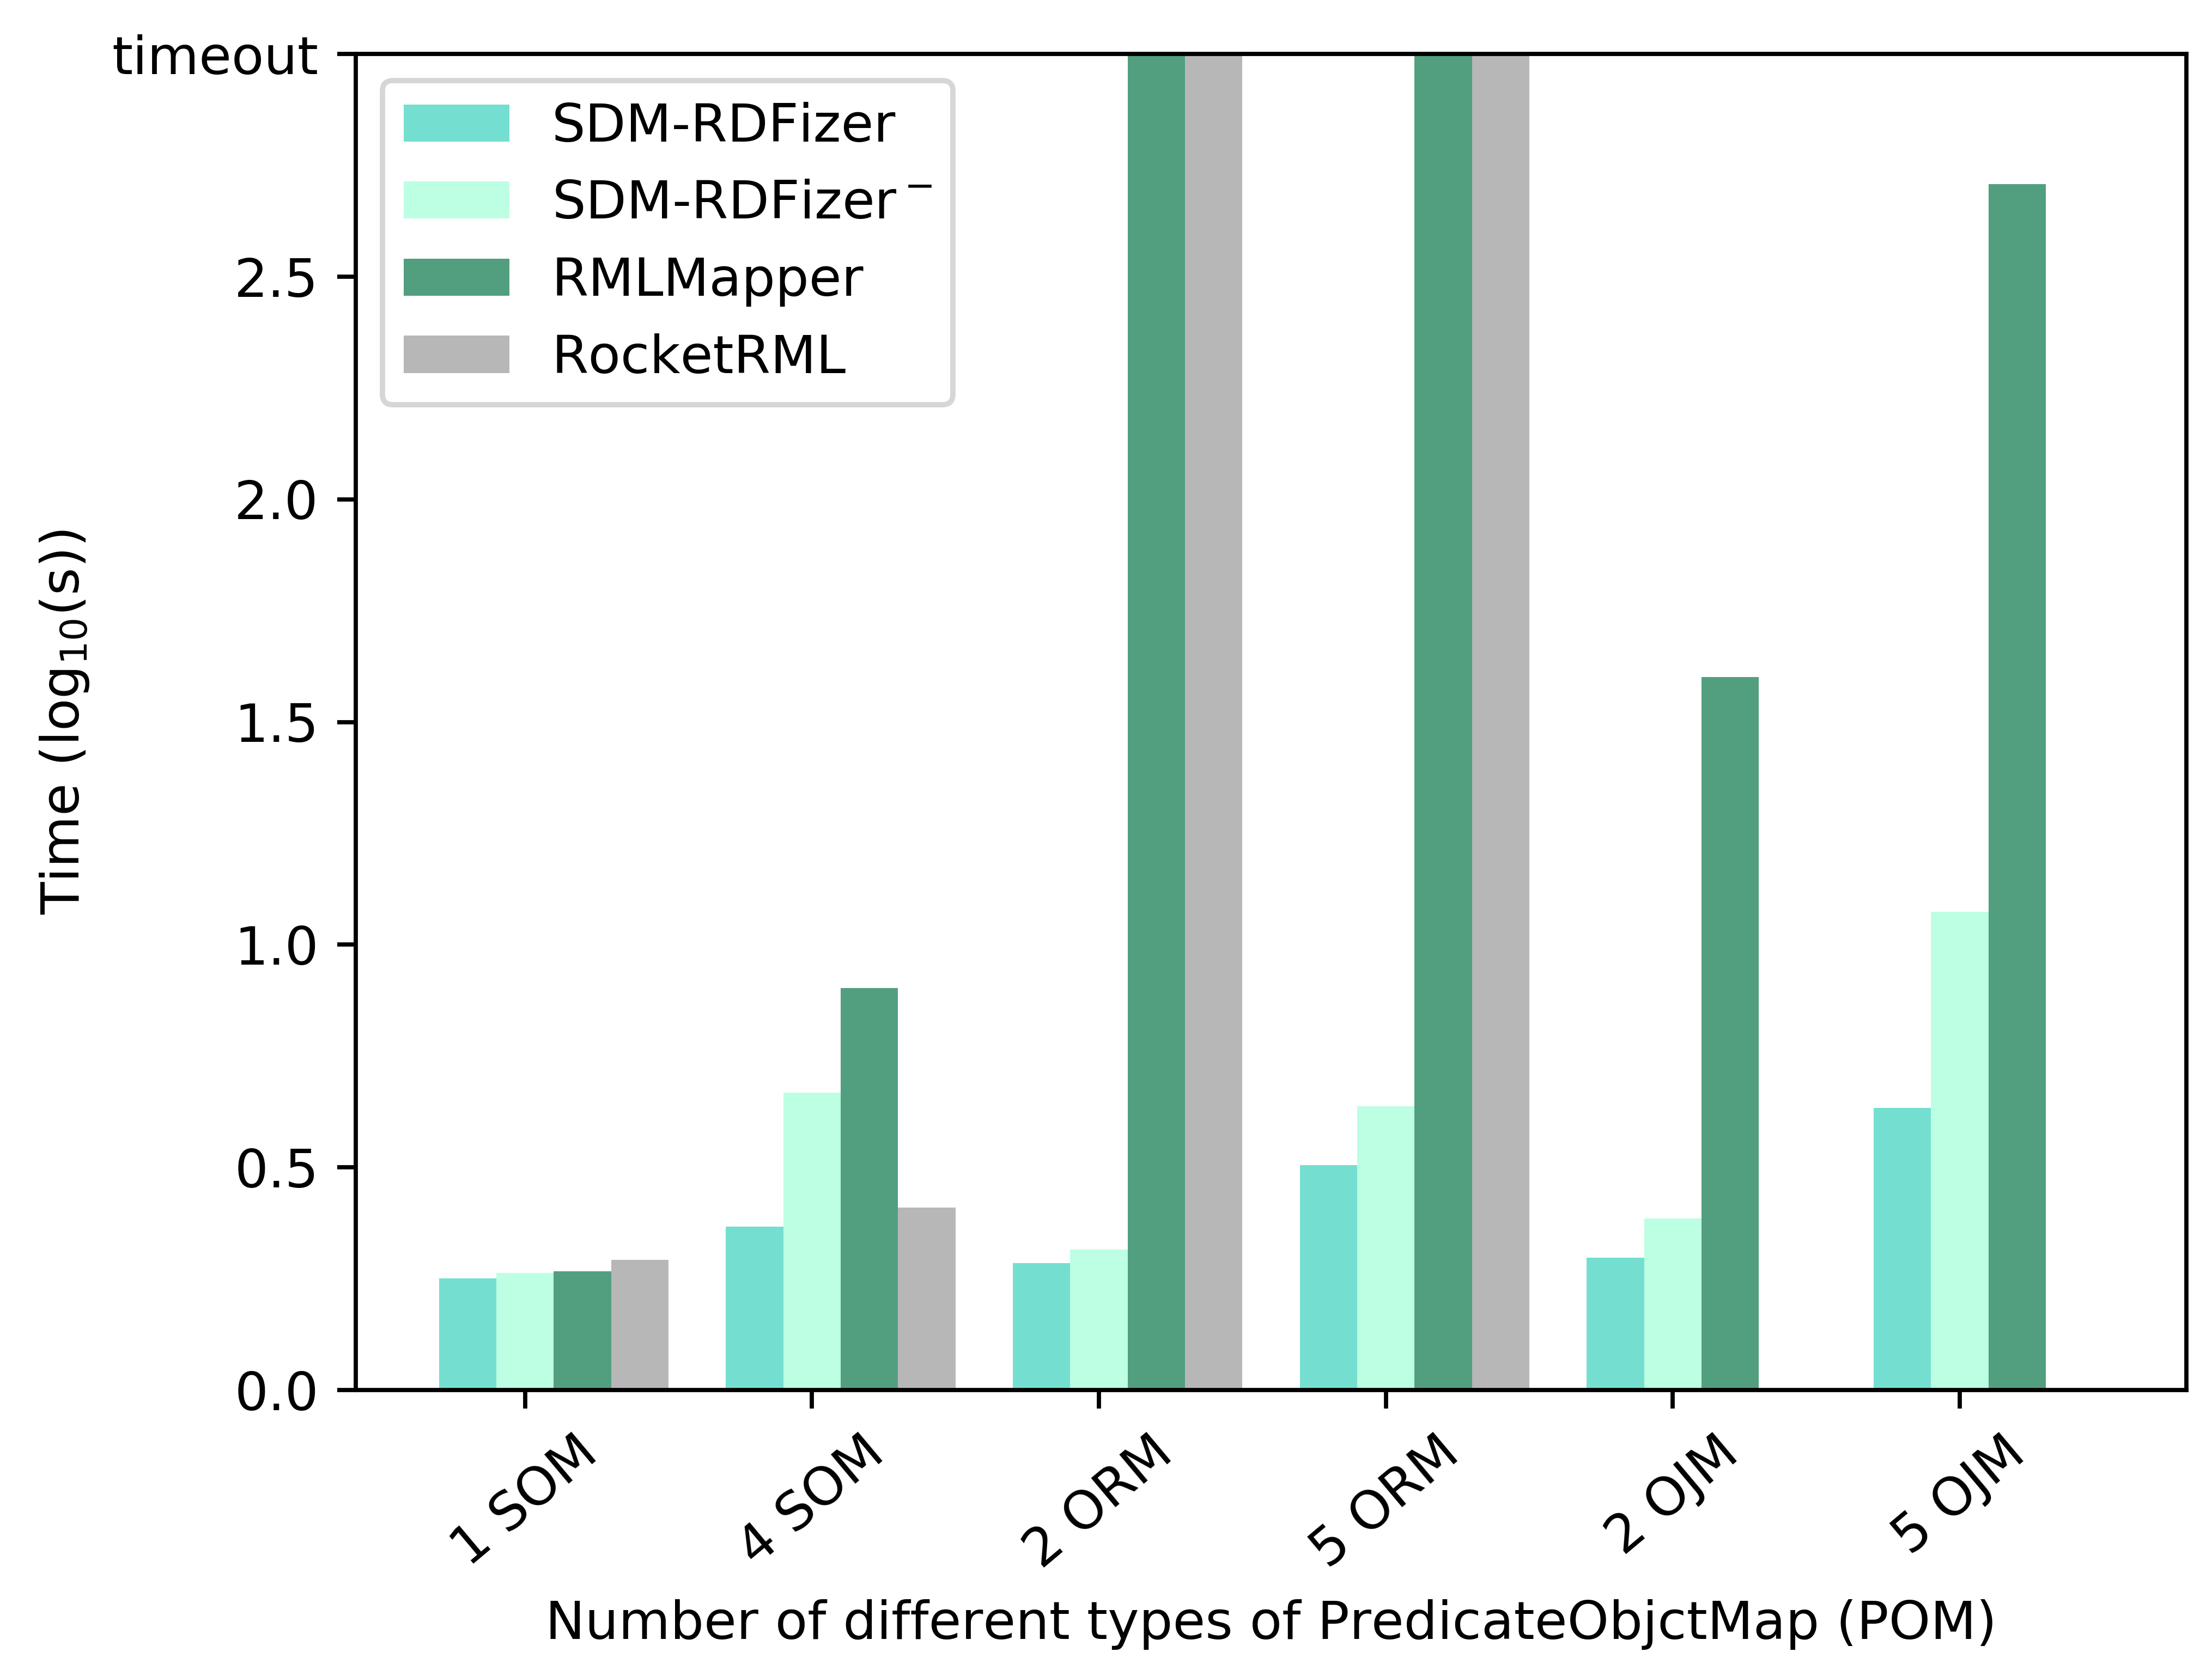
\includegraphics[width=0.45\columnwidth]{figures/sdmrdfizer/10k_vera75.png}
    \label{fig:vera75_10K}}
    \subfloat[100k records]{
    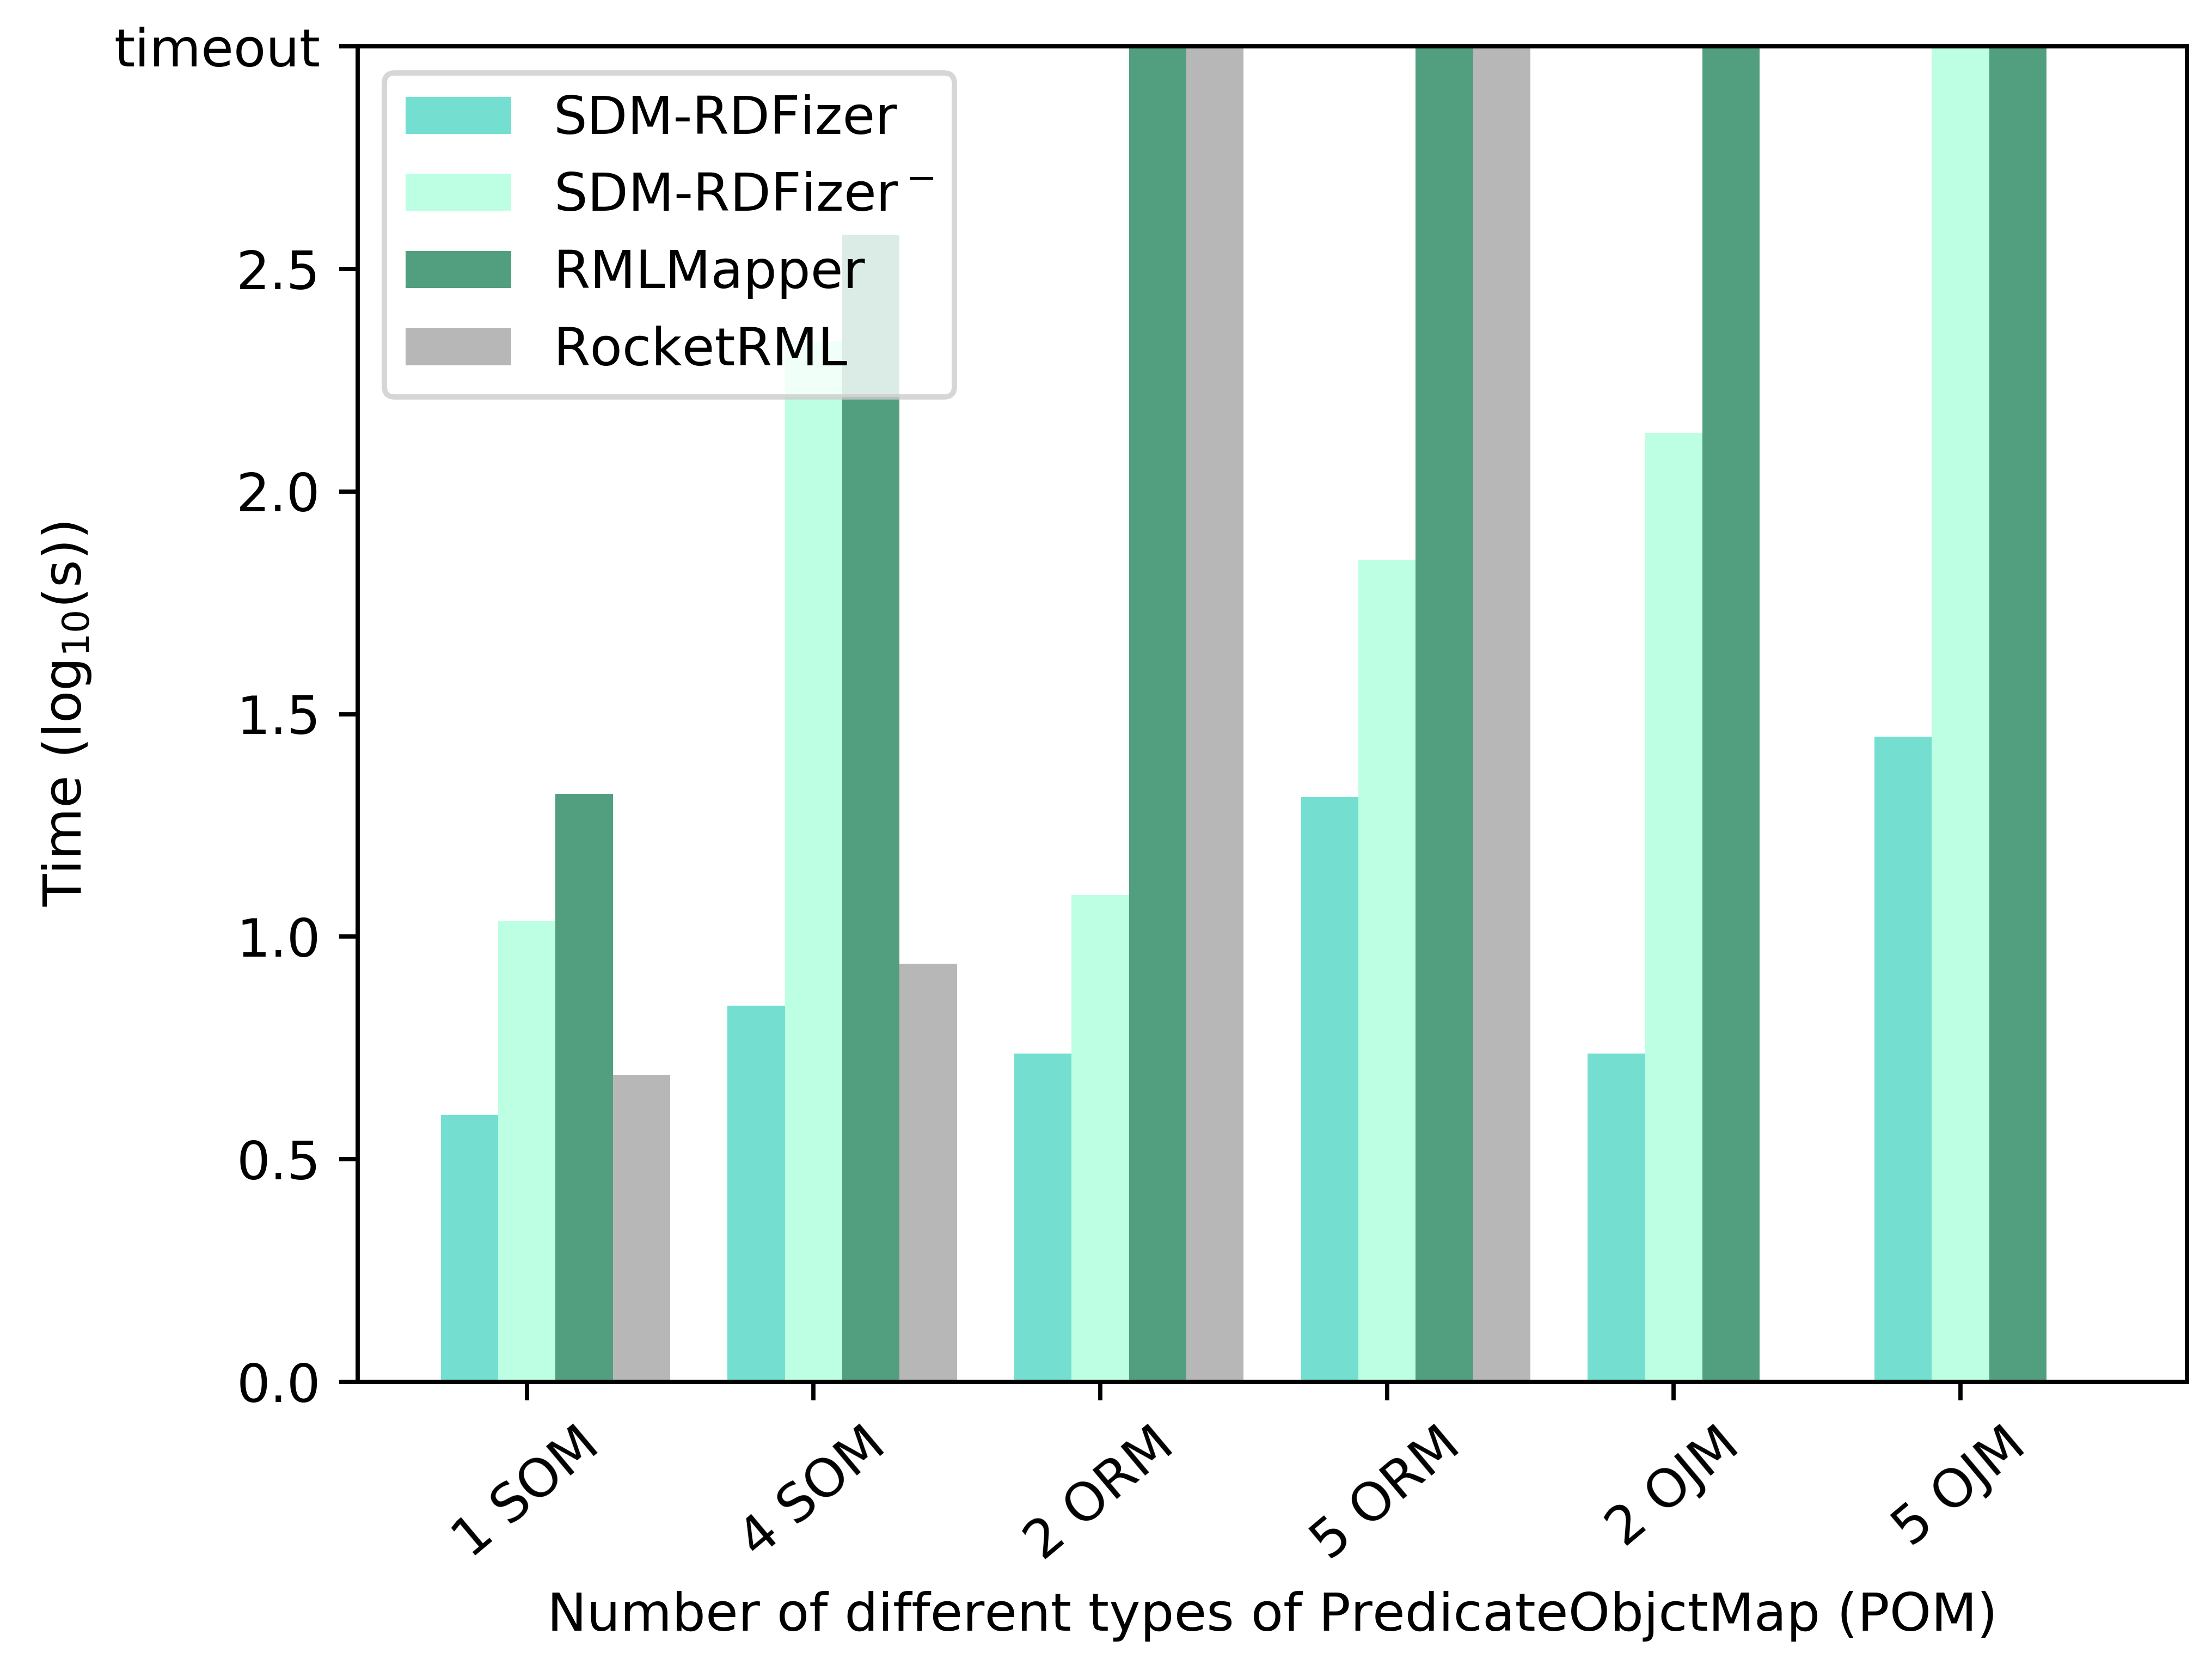
\includegraphics[width=0.45\columnwidth]{figures/sdmrdfizer/100k_vera75.png}
    \label{fig:vera75_100K}}
    \qquad
    \subfloat[1M records]{
    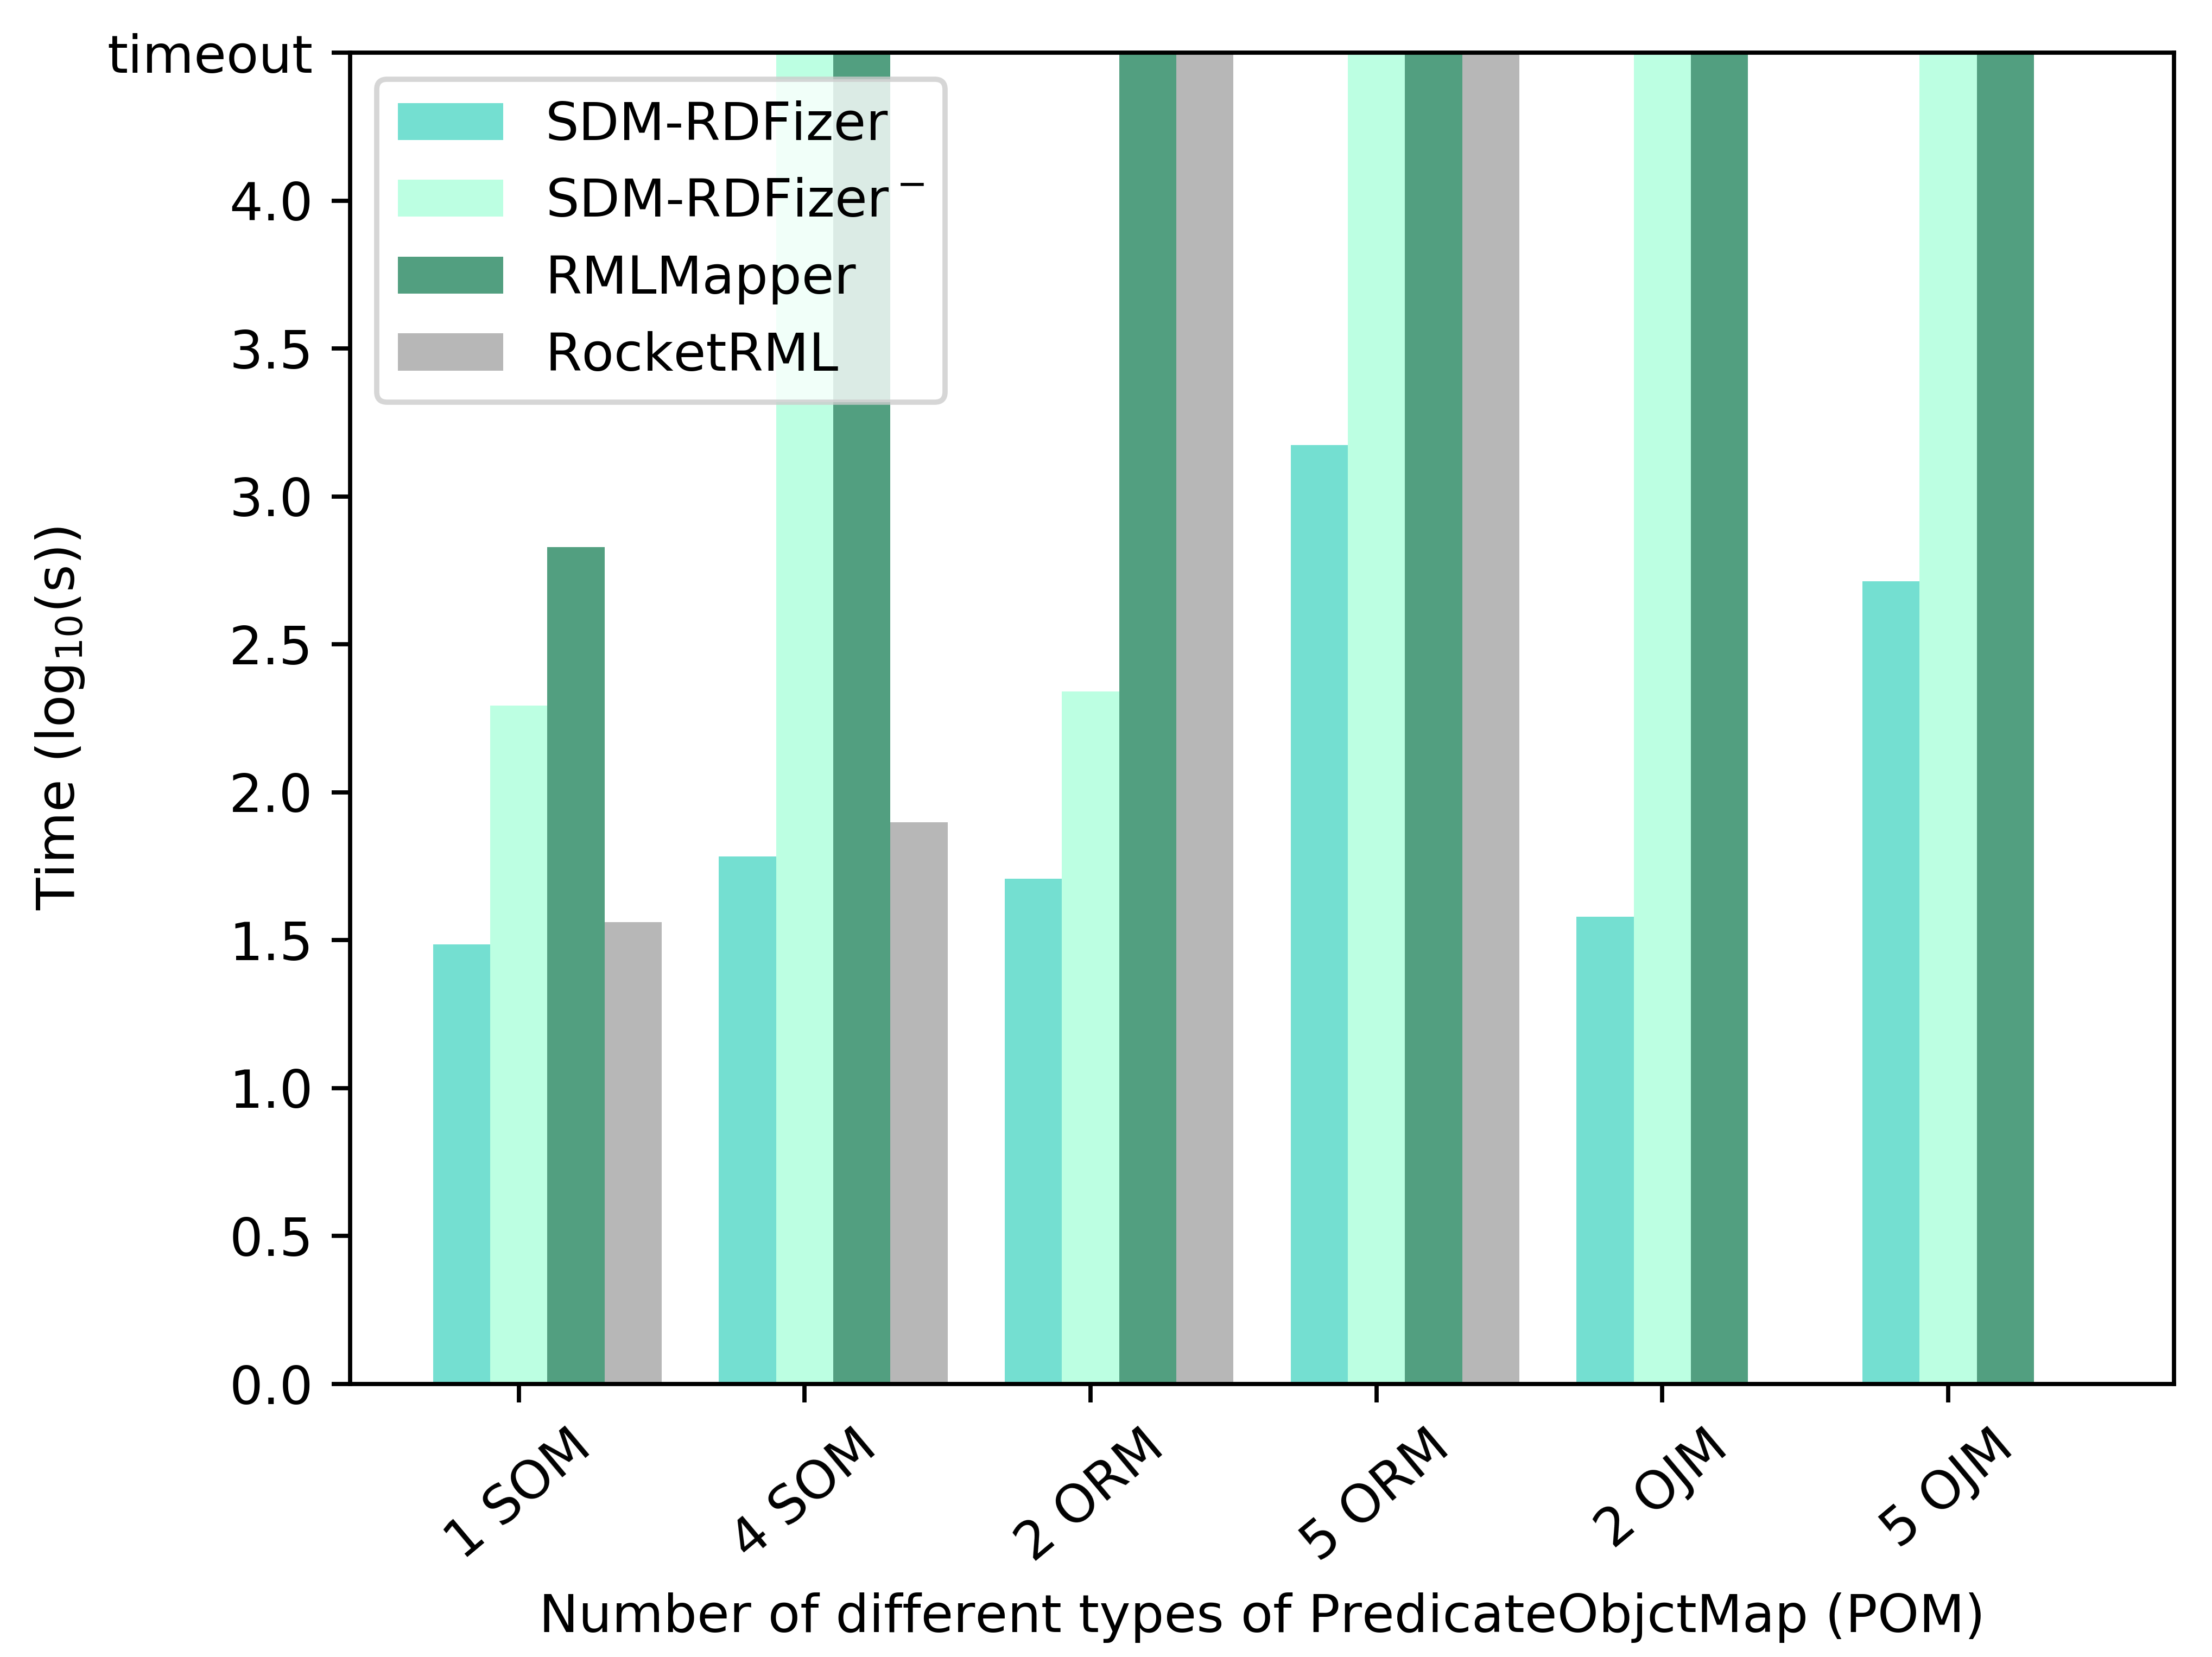
\includegraphics[width=0.45\columnwidth]{figures/sdmrdfizer/1M_vera75.png}
    \label{fig:vera75_1M}}
\caption[Execution time for with 75\% duplicates]{{\bf Total execution time of experiments on datasets with 75\% duplicates.}  SOM means simple object map, ORM object reference map and OJM object join map. RocketRML generates incorrect results running OJM mappings.}
\label{fig:75percent}
\end{figure}
\subsection{SDM-RDFizer as a Resource}

\textbf{Novelty:}
SDM-RDFizer introduces a novel set of operators to execute mapping rules in a data integration system; they allow for an efficient creation of knowledge graphs from heterogeneous data sources. Although the current version of SDM-RDFizer is customized for RML, the set of operators can be easily extended for other mapping rule languages and data models to represent knowledge graphs. Results of the experimental studies comparing the performance of SDM-RDFizer illustrate the novelty of the proposed work with the state of the art. We hope that these results encourage the community to advance existing approaches to scale up to the avalanche of available data that is expected in the next years.
\\
\textbf{Availability:}
SDM-RDFizer is released publicly by the Scientific Data Management (SDM) group at TIB, Hannover\footnote{\url{https://www.tib.eu/en/research-development/scientific-data-management/}}. 
TIB is one of the largest libraries for science and technology in the world, and following its policy of engaging open access to scientific artifacts, will keep available SDM-RDFizer as a tool for supporting the creation of knowledge graphs.  
The SDM-RDFizer is open source, written in Python 3, and available under the Apache License 2.0 license in an open Github repository\footnote{\url{https://github.com/SDM-TIB/SDM-RDFizer}}; it is regularly updated with new features. 
Additionally, following open science good practices, we register the tool at the Zenodo platform, which takes the Github repository and gives a general DOI\footnote{\url{https://doi.org/10.5281/zenodo.3872103}} to the engine and also a DOI for each release of the code\footnote{SDM-RDFizer v3.2:\url{https://doi.org/10.5281/zenodo.3872104}}. 
Thus, users and practitioners can use and cite a specific version of the engine, ensuring reproducibility and traceability of any experimental evaluation.
\\
\textbf{Utility:}
A docker image of SDM-RDFizer is available at DockerHub\footnote{\url{https://hub.docker.com/repository/docker/sdmtib/sdmrdfizer}} and the Github repository of the resource, provides a detailed explanation of how to create and run the Docker container. The use case presented in the motivating example is utilized to facilitate the understanding. Furthermore, the activity of commits in the Github repository evidence the attention paid to the creation of new versions, as well as to the resolution of the issues identified by the users of the tool.   
\\
\textbf{Predicted Impact:}
 The number of visits of knowledge graphs like DBpedia and Wikidata, and the current developments in scientific (e.g., \citep{AuerKPKSV18}) and industrial areas (e.g., \citep{NoyGJNPT19}) evidence the need of providing efficient tools for knowledge graph management at scale. Results of experimental evaluations of SDM-RDFizer illustrate the benefits of grounding solutions for the problem of knowledge graph creation in the well-established areas of data integration systems and query processing. Thus, we ambition that they will be the starting point of future developments, e.g., for the optimization and distribution of mapping rule executions, as well as for semantically enriching data integration systems whose execution enable the explainability of the whole process of knowledge graph creation. 
 \\
\textbf{Adoption and Reusability:}
Several projects from different domains already use SDM-RDFizer.
iASiS\footnote{\url{http://project-iasis.eu/}} and BigMedilytics - lung cancer pilot \footnote{\url{https://www.bigmedilytics.eu/}} are exemplary of EU H2020 projects.
The iASiS RDF knowledge graph comprises more than 1.2B RDF triples collected from more than 40 heterogeneous sources using more than 1300 RML triple maps, while 800 RML triple maps are used to create from 25 data sources, a lung cancer knowledge graph with 500M RDF triples. SDM-RDFizer has also created the \textit{Knowledge4COVID-19} knowledge graph during the EUvsVirus Hackathon\footnote{\url{https://blogs.tib.eu/wp/tib/2020/05/06/how-do-knowledge-graphs-contribute-to-understanding-covid-19-related-treatments/}}; it comprises 28M RDF triples describing 63527 COVID-19 articles and related COVID-19 concepts (e.g., drug-drug interactions and molecular disfunctions). SDM-RDFizer is also used in EU H2020, EIT-Digital, and Spanish national projects where the Ontology Engineering Group (Technical University of Madrid) participates. These projects, mainly focused on the transportation and smart cities domain, include: SPRINT\footnote{\url{http://sprint-transport.eu/}}, SNAP \footnote{\url{https://snap-project.eu/}} and Open Cities \footnote{\url{https://ciudades-abiertas.es/}}. Similar as the \textit{Knowledge4COVID-19} knowledge graph, SDM-RDFizer also created the Knowledge Graph of the Drugs4Covid project \footnote{\url{https://drugs4covid.oeg-upm.net/}} where NLP annotations and metadata from more than 60,000 COVID-19 articles are integrated in almost 44M RDF triples.

\subsection{Empirical Evaluation}

We compare SDM-RDFizer with a baseline and existing RML interpreters. We aim to answer the following research questions:
\begin{itemize}
\item Q1) What is the impact of data duplication rate in the execution time of a knowledge graph creation approach?
\item Q2) What is the impact of input data size in the total execution time of a knowledge graph creation process?
\item Q3) What is the effect of the triples map types in the \verb|PredicateObjectMap| of a RML mapping affect the existing engines?
\end{itemize}
All the resources used in this evaluation are publicly available\footnote{\url{https://github.com/SDM-TIB/SDM-RDFizer-Experiments}}. The experimental configuration is as follows:

\noindent\textbf{Datasets and Mappings.} To the best of our knowledge, there is no testbeds to evaluate the performance of a KG creation approaches from heterogeneous data sources. Consequently, following the real-world scenario that initially motivated this research, we create our testbed from the biomedical domain. From the coding point mutation dataset in COSMIC\footnote{\url{https://cancer.sanger.ac.uk/cosmic} GRCh37, version90, released August 2019}, we randomly select records to create six datasets with different sizes, i.e., 10K, 100K, and 1M number of rows. Accordingly, each two datasets with the same volume size differ each other in the number of duplicated values; including 25\% or 75\% of duplicates with each duplicated value to be repeated 20 times. In total, three mapping files are created with different types of \verb|PredicateObjectMap|: Simple Object Map rules with reference to columns (SOM), Object Reference Map rules (ORM) and Object Join Map rules (OJM). Each type of rules also varies from 1 to 4 number of \verb|PredicateObjectMap|.

\noindent\textbf{Engines.} The SDM-RDFizer v3.2 is tested in two different configurations: optimized version including the proposed operators (SDM-RDFizer) and the baseline with the na\"ive operators (SDM-RDFizer$^-$). Additionally, we also run the experiments over two well-known RML-compliant engines: RMLMapper v4.7\footnote{\url{https://github.com/RMLio/rmlmapper-java}} and RocketRML v1.7.0\footnote{\url{https://github.com/semantifyit/RocketRML/}}. There is available a docker image per tested engine to facility reproducibility of the study.

\noindent\textbf{Metrics.} \textit{Execution time:} Elapsed time spent by an engine to complete the creation of a knowledge graph; it is measured as the absolute wall-clock system time as reported by the \verb|time| command of the Linux operating system. \textit{Number of RDF triples} in the knowledge graph. Each experiment was executed five times and average is reported. The time out is set to 5 hours. The experiments were run in an Intel(R) Xeon(R) equipped with a CPU E5-2603 v3 @ 1.60GHz 20 cores, 64GB memory and with the O.S. Ubuntu 16.04LTS.

%\noindent\paragraph{\textbf{{Discussion of Observed Results.}}}
\subsubsection{Discussion}
In this section, we describe the outcomes of our experiments evaluating the performance of the selected engines (i.e., SDM-RDFizer, RMLMapper, and RocketRML) in different testbeds.
\autoref{fig:25percent} and \autoref{fig:75percent} report on execution time for creating a knowledge graph from datasets with 25\% and 75\% of duplicates, respectively. It should be noted that since RocketRML does not support N-M join relations and generates incorrect outputs subsequently, we only provide the results of SOM and ORM mappings for this engine. For the rest of the experiments, we have verified that the generated outputs are the same for all the approaches in terms of cardinality and correctness.\\
\noindent The obtained results clearly reveal the benefits of applying the proposed operators during the process of creating a knowledge graph. As illustrated in \autoref{fig:25percent} and \autoref{fig:75percent}, independent of the size of the input datasets and the percentage of existing duplicates, RMLMapper and RocketRML fail to generate RDF triples from mappings including 2-ORM and 5-ORM; they time out in five hours. Moreover, the execution time of RMLMapper and RocketRML increases as the size of data and number triples maps increase. Nonetheless, as it can be observed, SDM-RDFizer completes the RDF triples generation in all testbeds within a reasonable time period. Additionally, the performance of SDM-RDFizer$^-$ provides evidence of the quality of the SDM-RDFizer operators and their ability of speeding up a knowledge graph creation process.       


\subsection{Conclusions}

The observation that both industrial and scientific applications demand efficient solutions for knowledge graph creation motivated the need of making SDM-RDFizer available as a resource. SDM-RDFizer implements novel physical operators and data structures that speed up the generation of duplicate-free RDF triples even in presence of data sources with high-duplication rate. Empirical results indicate that SDM-RDFizer outperforms the state of the art by up to three orders of magnitude. Thus, SDM-RDFizer broaden the portfolio of technologies for knowledge graph management and provides the basis for the development of real-world knowledge graph applications. In the future, we plan to devise optimization techniques to plan the execution of the mapping rules, as well as to extend SDM-RDFizer to other mapping languages.

\definecolor{powderBlue}{RGB}{147, 207, 207}
\definecolor{blueGreen}{RGB}{89, 189, 192}
\definecolor{metallicSeaweed}{RGB}{6, 134, 146}
\definecolor{viridianGreen}{RGB}{1, 146, 150}
\definecolor{burntSienna}{RGB}{220, 120, 85}
\definecolor{melon}{RGB}{246, 183, 161}
\definecolor{rust}{RGB}{190, 51, 2}
\definecolor{grey}{RGB}{183, 183, 183}

\section{Efficient Processing of Functional Mappings for KG Materialization}
\label{chap7_funmap}
Function-based mapping languages \citep{de2017declarative,debruyne2016r2rml,junior2016funul,vu2019d} are equipped with abstractions that enable interoperable and reusable specifications of data transformations by means of user-defined functions as we described in Section \ref{soa2:functions}. Formalisms like RML+FnO~\citep{de2017declarative} combine the Function ontology and RML, enabling declarative specification of the schema-ontology alignments and data transformations that define the process of KG construction. Albeit expressive, existing mapping languages lack efficient interpreters able to scale up to complex KG construction scenarios. 

Extending the work proposed in Section \ref{chap7_rdfizer}, we tackle the problem of scaled-up KG construction from functional mapping rules and study the impact of functions when applied to large data sources with a high data duplication rate. Mappings among data sources and the system ontology are expressed using the RDF mapping language (RML) \citep{de2017declarative} and the Function Ontology (FnO); they define how the ontology concepts are populated with data from the sources in the resulting KG. We aim at transforming complex data integration systems composed of large data sources and mappings with functions into equivalent ones that generates the same KG but in less time (i.e., proposing a horizontal solution to enhance current KGC workflows)

FunMap is an interpreter of RML+FnO, that converts a data integration system defined using RML+FnO into an equivalent one where RML mappings are function-free. FunMap resembles existing mapping translation proposals (e.g., \citep{AliW19,corcho2019towards,junior2016funul}) and empowers a KG construction process with optimization techniques to reduce execution time. Transformations of data sources include the projection of the attributes used in the RML+FnO mappings. They are supported on well-known properties of the relational algebra, e.g., the pushing down of projections and selections into the data sources, and enable not only the reduction of the size of data sources but also the elimination of duplicates. Additionally, FunMap materializes functions --expressed in FnO-- and represents the results as data sources of the generated data integration system; the translation of RML+FnO into RML mappings that integrate the materialization of functions is performed using joins between the generated RML mappings. The combination of data source and function transformations results in data integration systems where only the data required to execute the RML mappings are retained. The computation of the functions used in the original data integration system is performed once. As a result, the new data integration system's execution is sped up while the same knowledge graph is generated. 

The contributions of this Section are: i) FunMap, an interpreter of RML+FnO that resorts to syntax-based translation~\citep{aho1986compilers} to push down projections and selections, and materialize functions. ii) Empirical evaluations of the performance of FunMap in real-world testbeds with data of various formats (CSV and Relational), sizes, and degrees of duplication that show reductions in KG construction time by up to a factor of 18.

\subsection{Applying functions in the Biomedical Domain: Motivating Example}

\begin{figure}[t!]
\centering
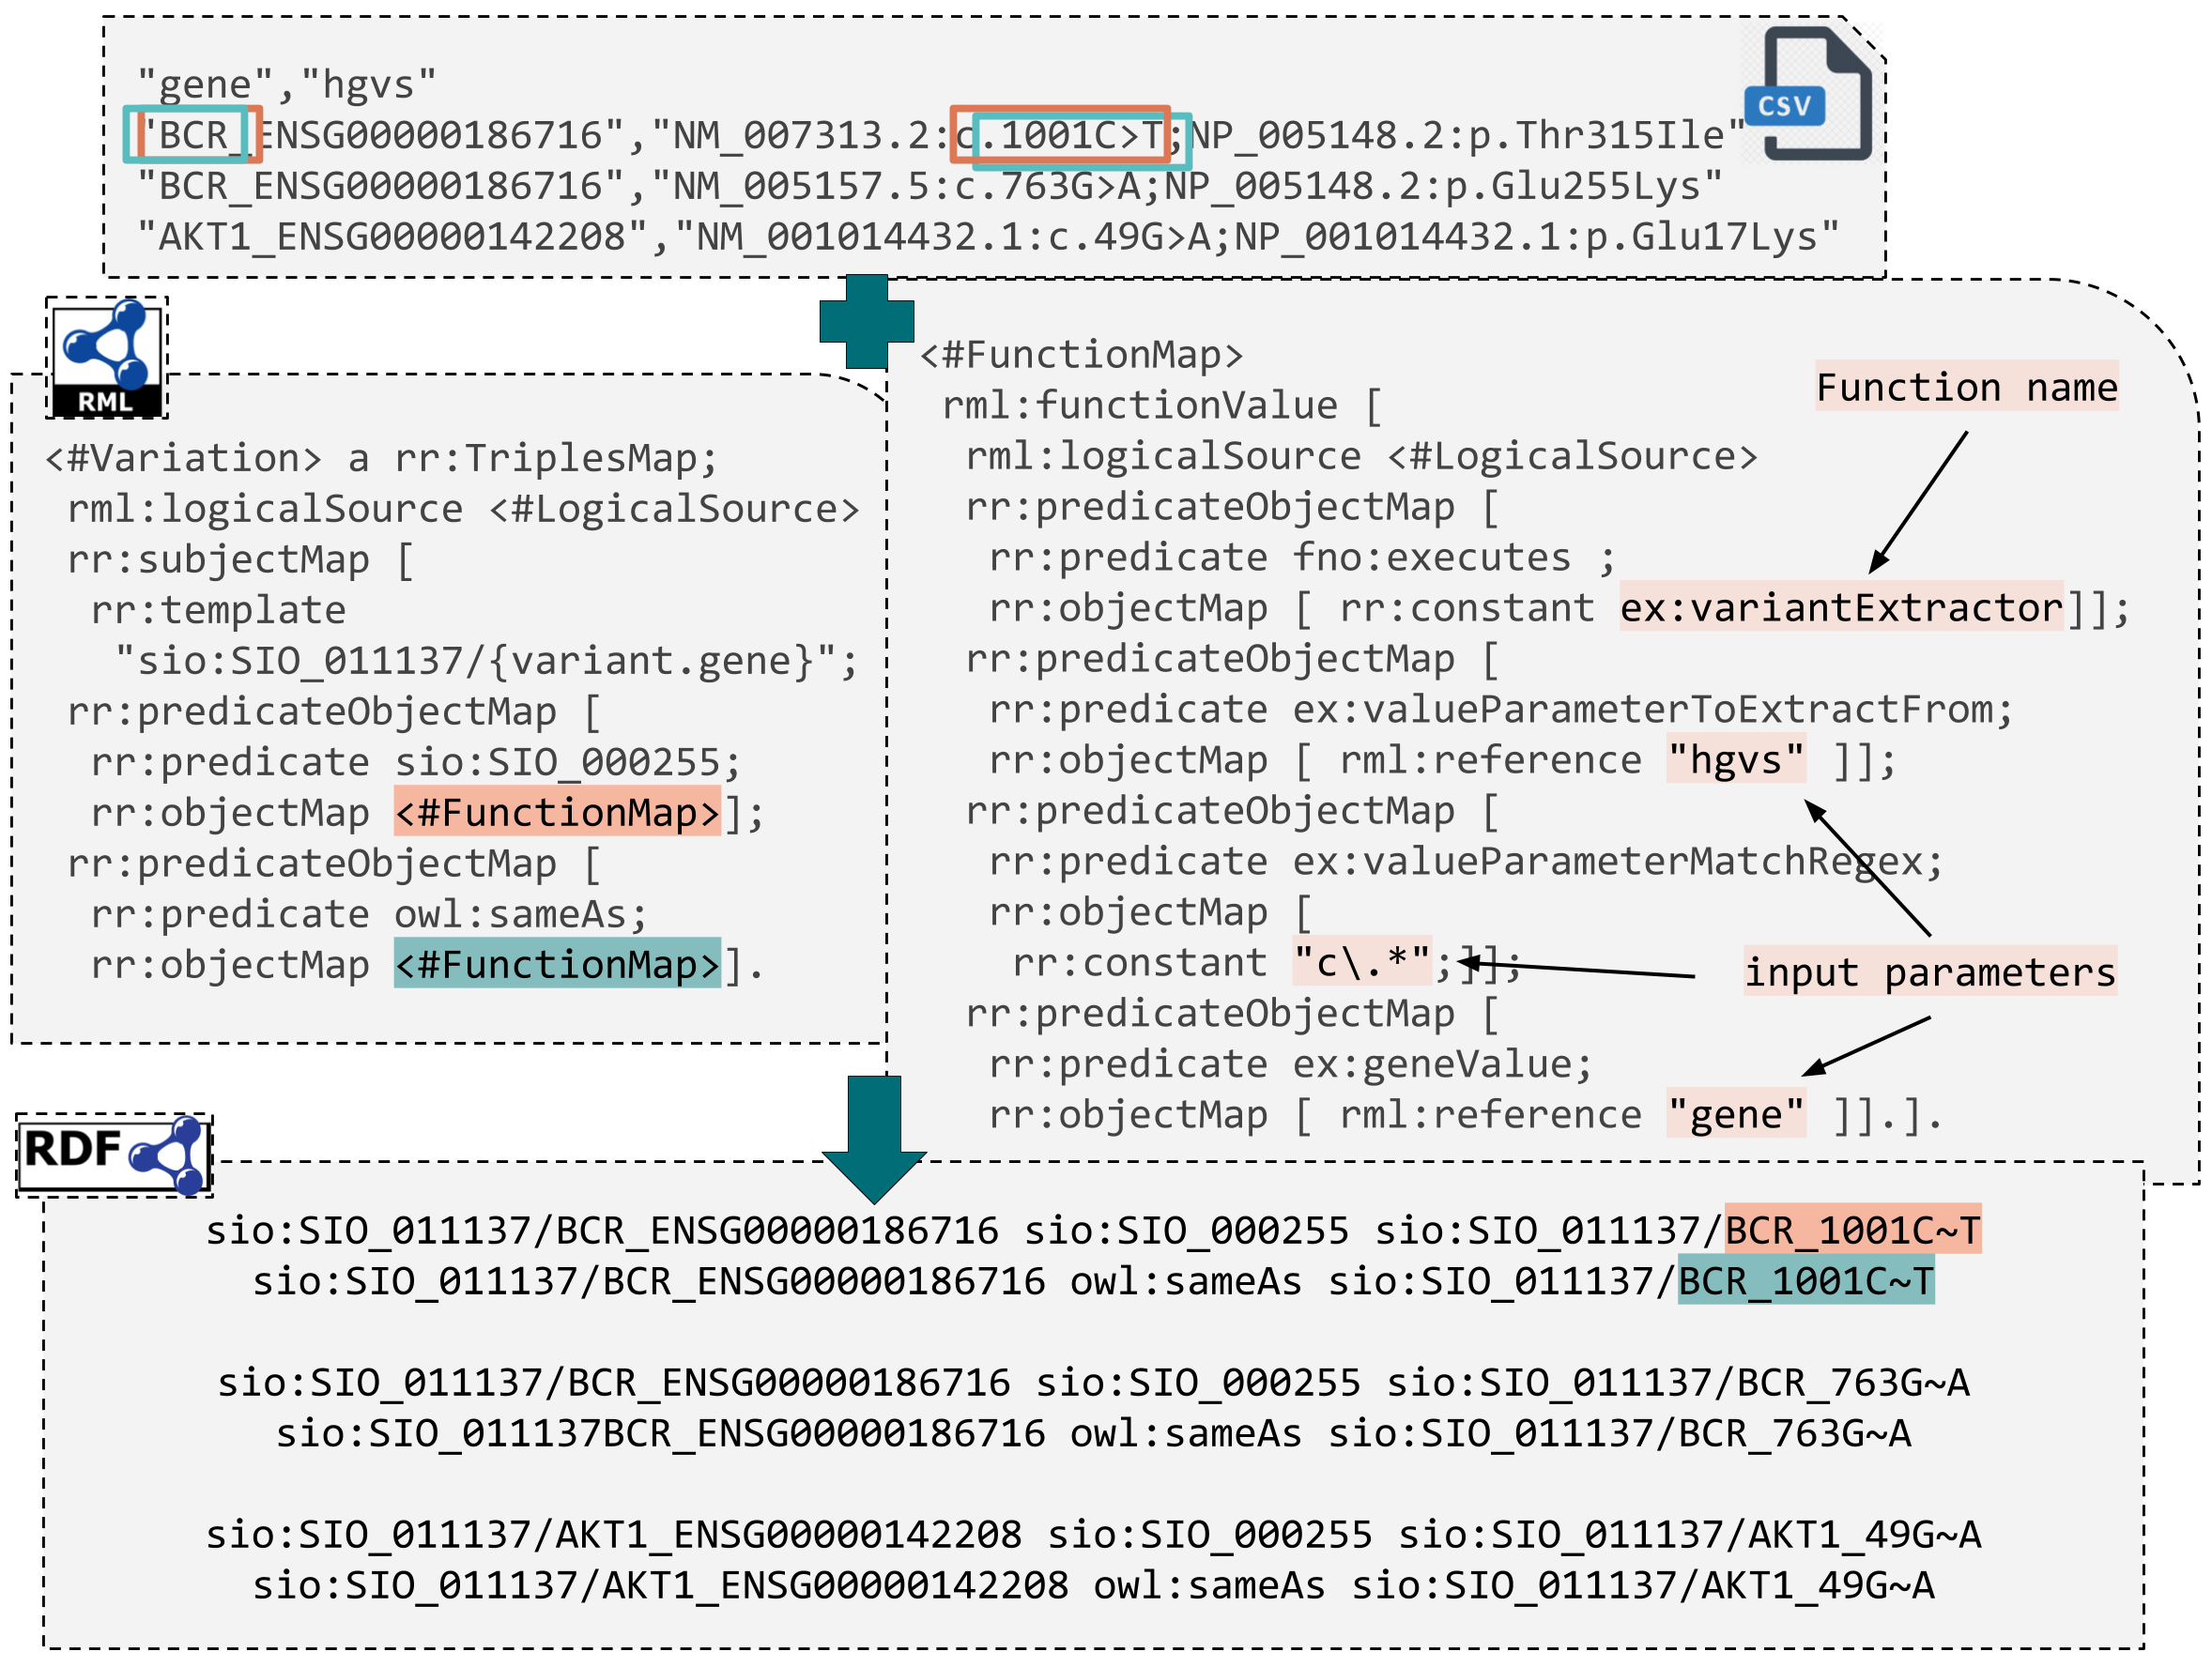
\includegraphics[width=\textwidth]{figures/motivating_example.png}
\caption[FunMap motivating example]{\textbf{Motivating example.} Knowledge graph construction using RML+FnO mapping rules for the biomedical domain. The input source in the top is transformed to RDF output (at the bottom) through the processing of the mapping (middle) where the transformation functions are defined. Repeated computations of a function negatively impacts on the performance of an RML engine.} 
\label{fig:motivatingExampleFunMap}
\end{figure}

Our work is motivated by the challenges revealed during genomic variant reconciliation while creating a biomedical knowledge graph. 
Although the vast majority of the single variations in the genome of a person causes no disease, benign variants can appear in sequenced genomic data repeatedly. In addition to the large heterogeneous volumes generated during genome sequencing and analysis, high-frequency of genomic variants impose data integration challenges while collecting genomic data from different sources. 
Additionally, genomic variants are expressed in diverse standard formats~\citep{den2016hgvs} and reported at DNA, RNA, or protein level. Moreover, this representation can be done according to any of the accepted terminologies and genomic reference versions. Unified representations for variants are required
to semantically recognize and integrate equivalent variants residing in different data sources. Variant representations can result from a composition of several factors, such as gene name, genomic position, and residue alteration. 
Pre-processing functions (e.g., FnO functions) are needed to extract and compose values from different attributes from each data source and generate such a combined representation of variants.
These functions are part of the data integration system's mapping rules that define the KG construction process. 

\autoref{fig:motivatingExampleFunMap} depicts a mapping rule in  RML+FnO where the \verb|FunctionMap| class is utilized. Consider that according to the \verb|LogicalSource| provided in this example, a \verb|FunctionMap| is defined in the mapping rules to create a unified representation for a variant by extracting the values of ``gene name'' (e.g., BCR) from the attribute \verb|gene| and 
``coding alteration'' (e.g., c.1001C\textgreater T)  from the attribute named \verb|hgvs| and combine them (e.g., BCR\textunderscore1001C\textasciitilde T). Current approaches evaluate \verb|FunctionMap| for each \verb|variant|, which can be expensive in presence of large data sources. Nevertheless, the large number of redundant values leaves room for the scalable transformations to execute functional mappings. 


\subsection{The FunMap Approach}

%\begin{table}[h!]
%\normalsize
%\centering
%\caption{Summary of the notation used for defining FunMap}
%\label{tab:notations}
%\resizebox{1.0\textwidth}{!}{%
%\begin{tabular}{|l|l|}
%\hline
%\textbf{Notation} & \textbf{Explanation} \\ \hline
%$DIS_G=\langle O,S,M \rangle$ & Data Integration System which creates a KG $G$ \\ \hline
%$O$ & Unified Ontology of $DIS_G=\langle O,S,M \rangle$\\ \hline
%$S$ & Finite set of Data Sources $S_i$ of $DIS_G=\langle O,S,M \rangle$\\ \hline
%$M$ & Finite set of \texttt{TriplesMap}s $T_i$ in $DIS_G=\langle O,S,M \rangle$\\ \hline
%$\emph{RDFize}(.)$ & A function producing RDF triples from a data integration system\\ %\hline
%$T'_i$ and $T'_k$ & \texttt{TriplesMap}s resulting of applying MTRs \\ \hline
%$F_i$ & A Transformation Function in a \texttt{TriplesMap} in $M$ \\ \hline
%$S'$ & Finite set of Data Sources $S'_i$ resulting of applying DTRs\\ \hline
%$M'$ & Finite set of Mapping Rules $M'_i$ resulting of applying MTRs\\ \hline
%$S_i^{output}$ & Data source resulting of applying DTR1, with attributes $o'_i$ and $a'_i$ %\\ 
%& representing the materialization of a transformation function $F_i$ \\ \hline
%$S_i^{project}$ &  Data source resulting of applying DTR2 \\ \hline
%\end{tabular}%
%}
%\end{table}
FunMap is an interpreter of data integration systems $DIS_G = \langle O,S,M \rangle$, where $O$ stands for a unified ontology, and $S$ and $M$ represent sets of sources and mapping rules, respectively \citep{Lenzerini02}. The evaluation of $DIS_G$ (a.k.a. $\emph{RDFize}(DIS_G)$) results into a knowledge graph $G$ that integrates data from $S$ according to the mapping rules in $M$; entities and properties in $G$ are described in terms of $O$. A complex data integration system $DIS_G$ consists of large data sources with high-duplicated data and mapping rules including functions for both schema-ontology alignments and data transformations. FunMap converts $DIS_G$ into an equivalent data integration system that creates the same knowledge graph but in less time.


\noindent\textbf{Problem Statement:} 
Given a data integration system $DIS_G$=$\langle O,S,M\rangle$, the problem of scaled-up knowledge graph creation from functional mappings requires the generation of a data integration system 
$DIS'_G$=$\langle O,S',M' \rangle$:
\begin{itemize}
\renewcommand{\labelitemi}{$\bullet$}
\item The knowledge graphs resulting of the evaluations of both data integration systems are the same, i.e., $\emph{RDFize}(DIS'_G = \langle O,S',M' \rangle)$=$\emph{RDFize}(DIS_G = \langle O,S,M \rangle)$ where $RDFize(.)$ is a function producing RDF triples utilizing the input data integration system.
%\item The execution time of evaluating $\emph{RDFize}(DIS'_G = \langle O,S',M' \rangle)$ is \emph{less} than $\emph{RDFize}(DIS'_G = \langle O,S',M' \rangle)$.
\item The execution time of $\emph{RDFize}(DIS'_G=\langle O,S',M' \rangle)$ is \emph{less than} the execution time of $\emph{RDFize}(DIS_G=\langle O,S,M \rangle)$.
\end{itemize}

\noindent \textbf{Solution:} FunMap implements a heuristic-based approach; it relies on the assumption that eliminating duplicates, maintaining in the data sources only the attributes mentioned in the mappings, and materializing the functions in the mappings, reduces the execution time of knowledge graph creation process. 
FunMap receives a data integration system $DIS_G$=$\langle O,S,M \rangle$ where the mappings $M$ are expressed in RML+FnO. FunMap interprets the mappings in $M$ and converts $DIS$ into the data integration system $DIS'_G$ in which the mappings $M'$ are function free and duplicates in the data sources $S'$ are reduced. \autoref{approach} depicts the FunMap approach; it performs a syntax-based translation of the mappings in $M$ and ensures that each redundant function is evaluated exactly once on the same data values. 
FunMap transforms $S$ to $S'$ by means of data transformation rules (DTR1 and DTR2). For each $F_i$ over a given $S_i$, DTR1 creates a temporal source $S'_i$ that includes the attributes from $S_i$ that correspond to the input of $F_i$; it also generates a source $S_i^{output}$ that contains the attributes in $S'_i$ and attributes representing the output of $F_i$. For each \verb|FunctionMap| defined over a source $S_i$, DTR2 creates a source $S_i^{project}$ that includes all attributes of $S_i$ used in the \verb|FunctionMap|. Additionally, FunMap converts mapping rules that include functions by using mapping transformation rules (MTRs); a \verb|FunctionMap| is transformed into \verb|FunctionMap|s without functions while connected by \verb|joinCondition|s; initially, $S'$ and $S$ are equal, as well as $M'$ and $M$. Properties \ref{property:p1}, \ref{property:p2}, and \ref{property:p3} state the pre- and post-conditions of DTRs and MTRs.

\begin{figure}[t!]
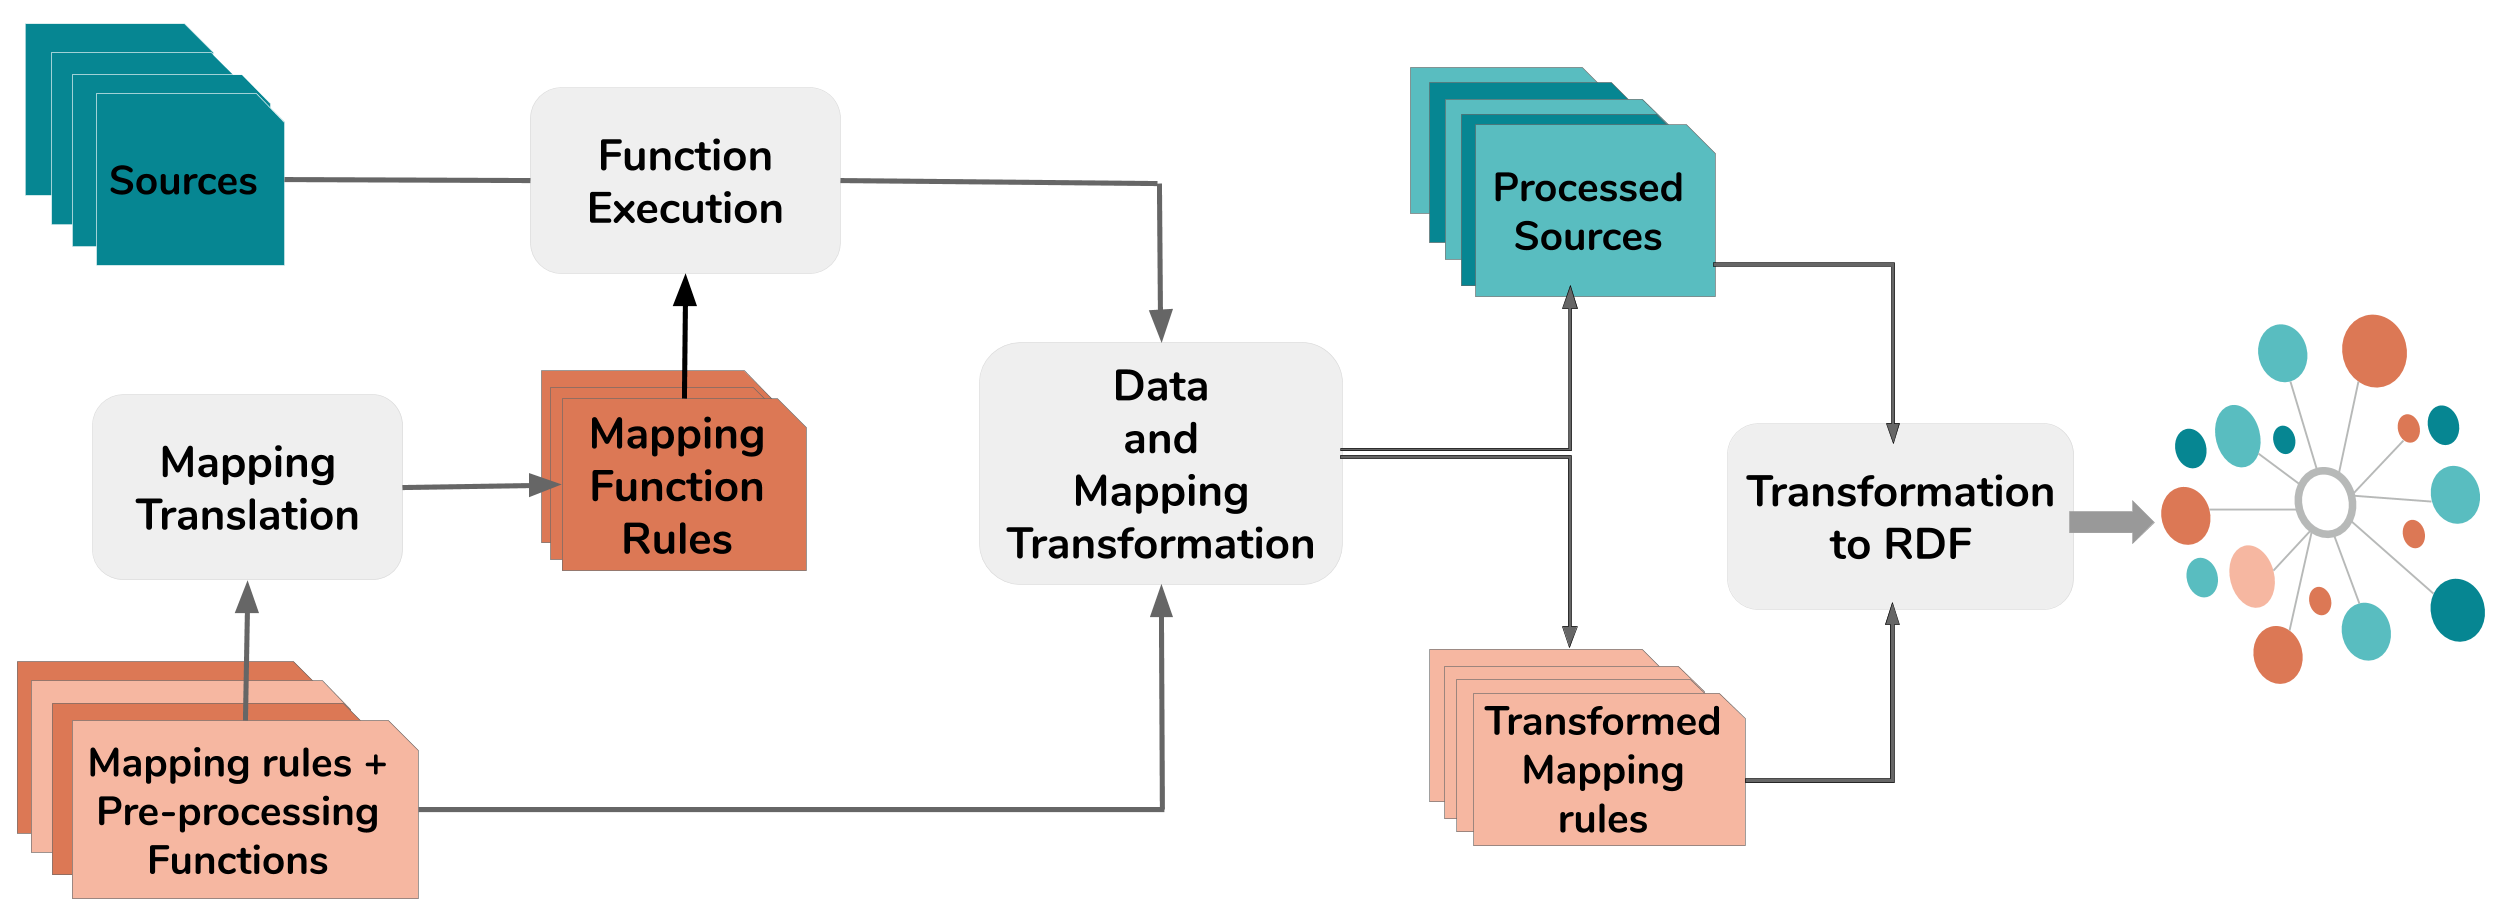
\includegraphics[width=\textwidth]{figures/Architecture.png}
\caption[The FunMap approach]{\textbf{The FunMap approach}} 
\label{approach}
\end{figure}


\subsubsection{Transformation Rules in FunMap}
\label{subsec:transformation}
\begin{figure}[t!]
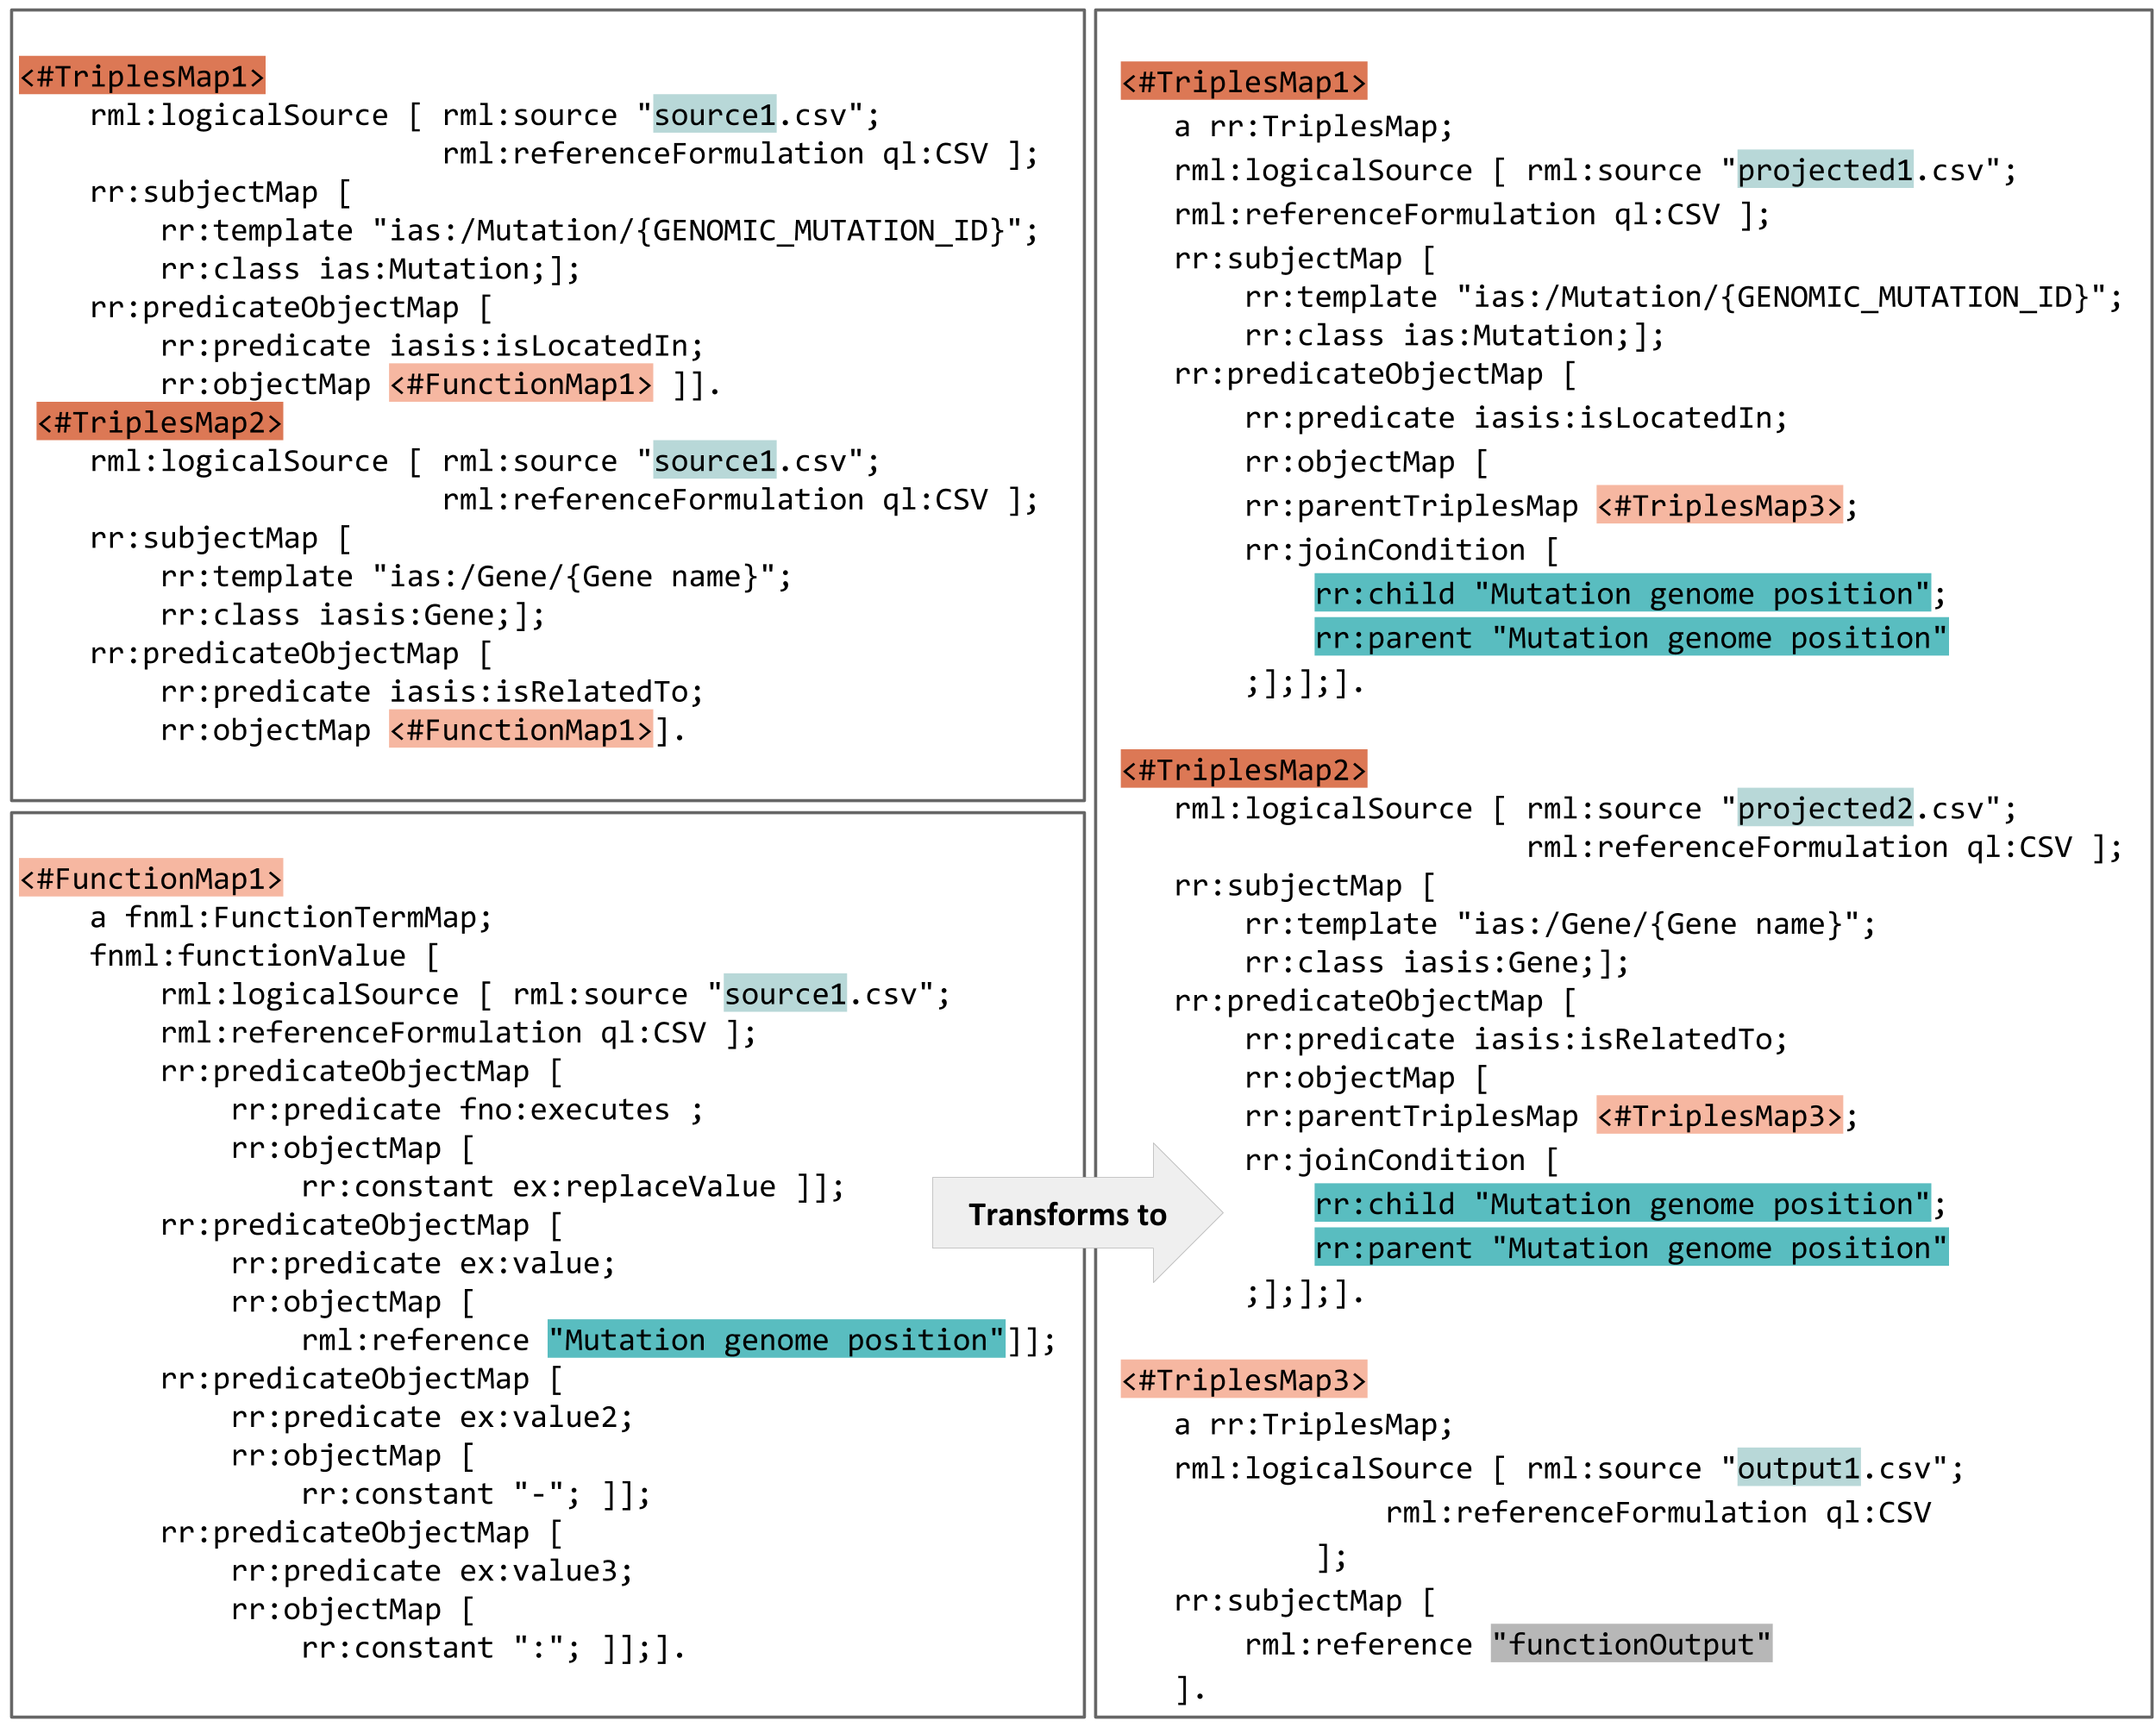
\includegraphics[width=\textwidth]{figures/MTR_objectBased.png}
\caption[DTR and Object-based MTR examples]{\textbf{Example of DTR and Object-based MTR.} On the left, an exemplary mapping including two TriplesMaps and a FunctionMap provided by the original data integration system. On the right side, the mappings are transformed by FunMap including two new TriplesMaps and one new TriplesMap.} 
\label{fig:objectBased}
\end{figure}
The FunMap syntax-based translation component parses \verb|FunctionMap|s exactly once, i.e., \verb|FunctionMap|s repeated in various mappings are not evaluated more than once. Given \verb|FunctionMap|s, original data sources, and mappings, FunMap executes transformation rules on data sources and mappings, accordingly. Meanwhile, given the transformed data sources, FunMap detects that a \verb|FunctionMap| has been computed for a given value and avoids repeating this computation. As an outcome, FunMap provides: a) a new set of data sources $S'$ consisting of the original ones in conjunction with transformed data sources,  and b) a set $M'$ of transformed function-free mappings. FunMap is loyal to the formats of data sources and mappings. Thus, any RDF mapping language is compatible with the process implemented in FunMap, as far as the language enables the definition of joins between mapping rules. Next, we present the transformation rules. 

\noindent\textbf{Data Source Transformation Rules (DTRs):}
Considering the fact that a \verb|TriplesMap| may only be used some attributes of a dataset, FunMap relies on the properties of the relational algebra and performs DTRs to project only the attributes mentioned in the \verb|TriplesMap|. DTRs are followed by transformation rules (MTRs) that update mappings defined over the transformed data sources. 

\noindent\textbf{DTR1: Projection of Functional Attributes:}
For each transformation function $F_i$ over a given source $S_i$ in the set of data sources $S$, FunMap projects all attributes $a'_i$ in $S_i$ that are input attributes of $F_i$, into a temporal data source $S'_i$ followed by duplicate removal. Subsequently, it evaluates $F_i$ over $S'_i$ and stores the results into the attribute $o_i$. Lastly, it creates a new data source $S_{i}^{output}$ with the attributes $a'_i$ and $o_i$; $S_{i}^{output}$ is added to $S'$. 
\begin{figure}[t!]
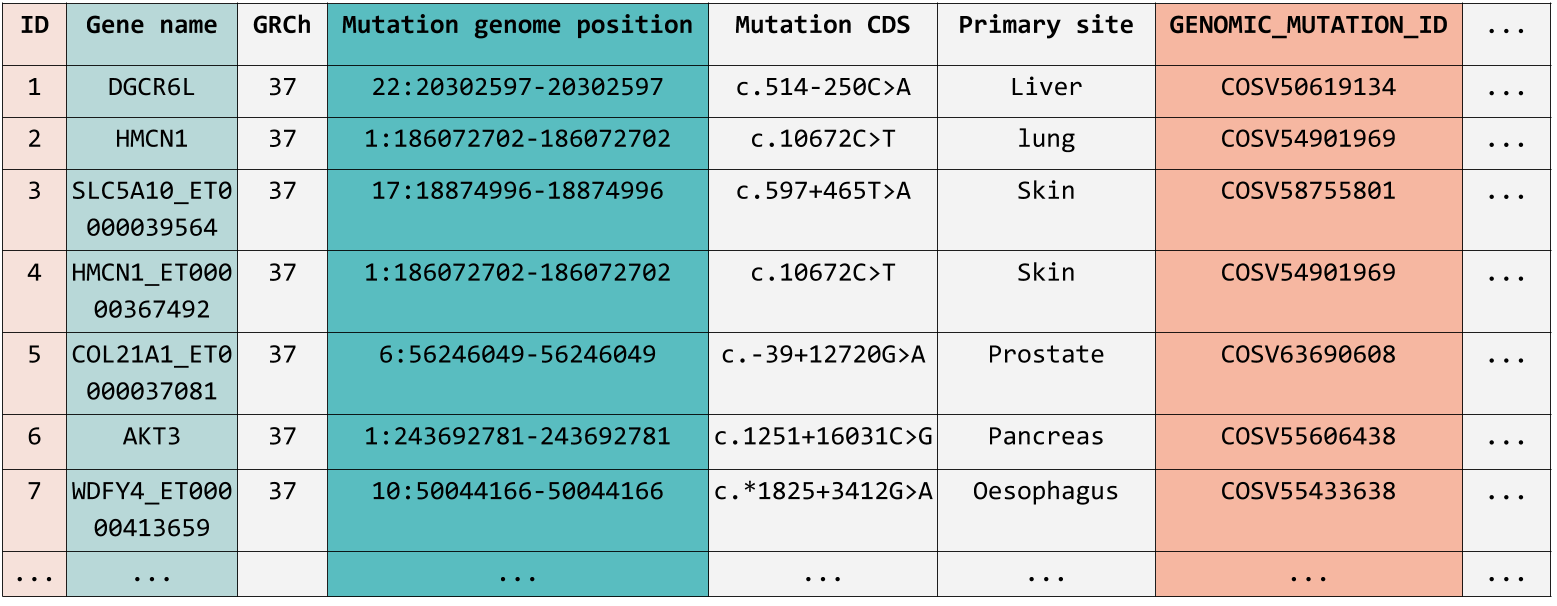
\includegraphics[width=\textwidth]{figures/OriginalDatasource.png}
\caption[Original input data source used by FunMap in KGC workflow]{\textbf{Original input data source used by FunMap in KGC workflow.} The data source includes many attributes among which only a few are required by the transformation function or function-free mappings in the process of knowledge graph creation.} 
\label{fig:OriginalDatasource}
\end{figure}
\begin{figure}[t!]
 \centering
 \subfloat[Projected1]{
      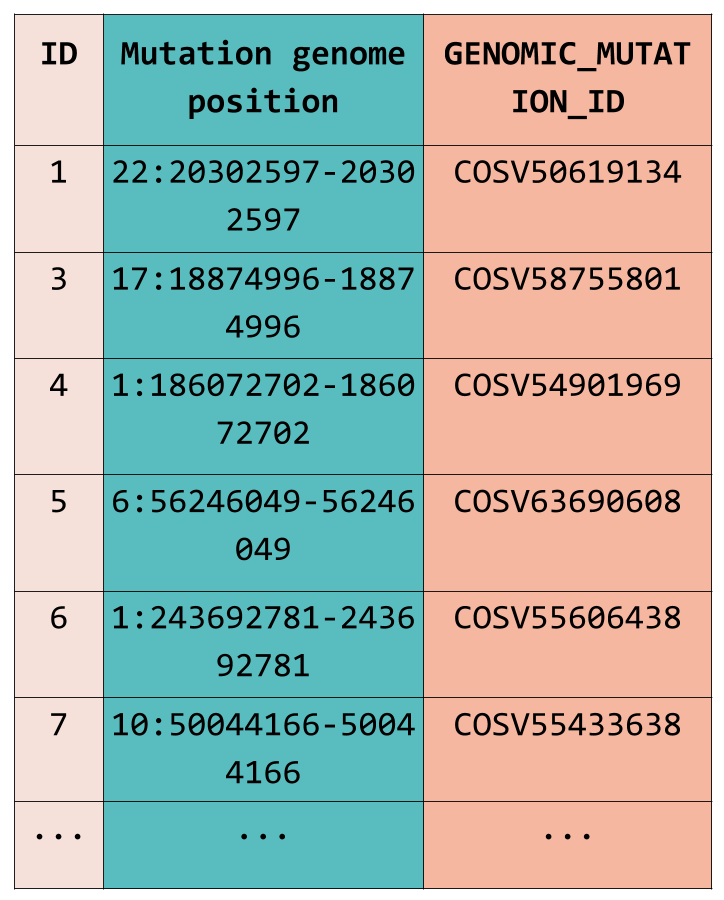
\includegraphics[width=0.32\columnwidth]{figures/DTR-projected1.png}
    \label{fig:projected1}}
  \subfloat[Projected2]{
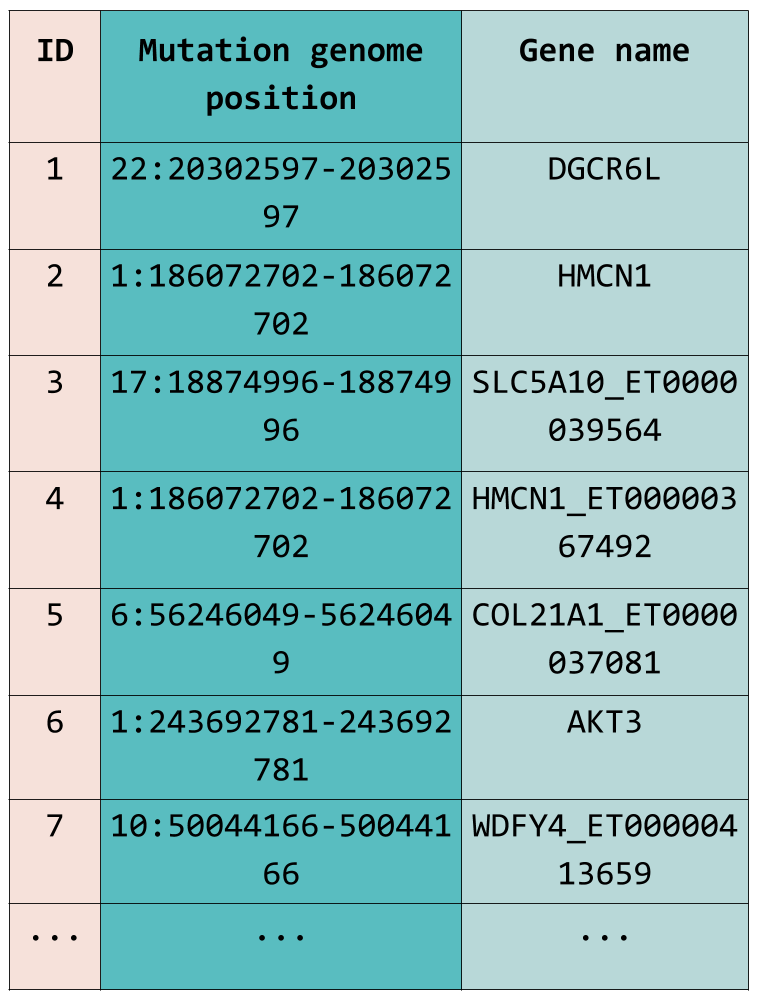
\includegraphics[width=0.32\columnwidth]{figures/DTR-projected2.png}
    \label{fig:projected2}}
  \subfloat[Output1]{
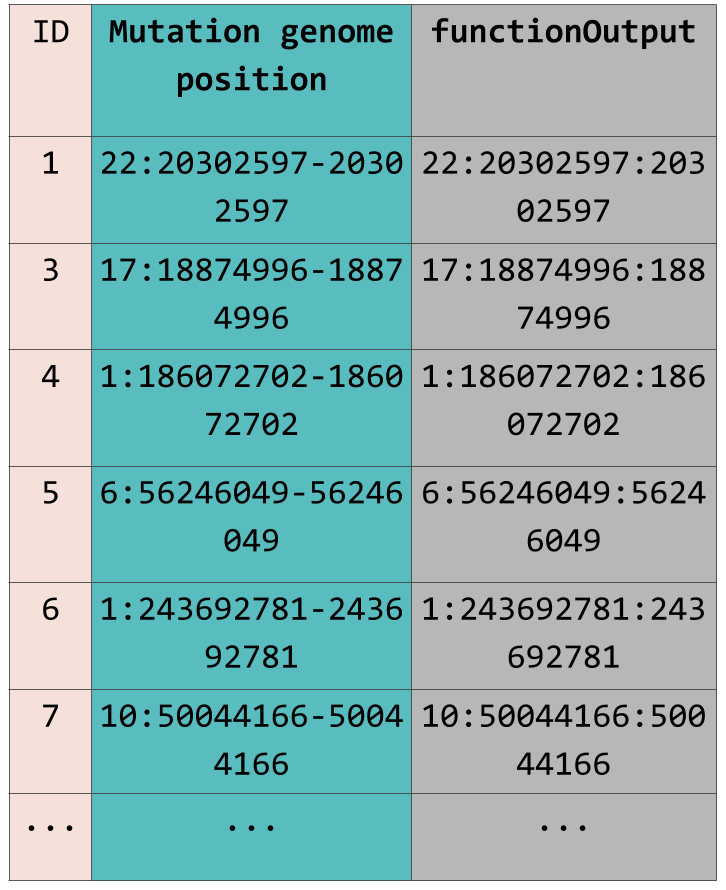
\includegraphics[width=0.32\columnwidth]{figures/DTR-output1.png}
    \label{fig:output1}}
    \caption[ Transformed sources generated by FunMap]{{\bf Transformed sources generated by FunMap.} The DTR2 generates a new source by projecting attributes for each TripleMap (Figures a and b) while DTR1 projects input and output attributes of each FunctionMap into a new source (Figure c). Both remove the generated duplicates.}
    \label{fig:funmap-dtr}
\end{figure}

\noindent\textbf{DTR2: Projection of Non-Functional Attributes:}
FunMap provides an additional DTR to further optimize the knowledge graph creation process. Exploiting transformation rules that are proposed in~\citep{jozashoori2019mapsdi}, FunMap projects all attributes in $S_i$ that are needed by \verb|TriplesMap| including those that are received by \verb|FunctionMap| as input into a new data source $S_i^{project}$ which is added to $S'$. 
To better conceive DTRs, consider the original mappings in \autoref{fig:objectBased} (left-side) and corresponding data source \verb|source1.csv| that can be seen in \autoref{fig:OriginalDatasource}. As shown in \autoref{fig:objectBased}, \verb|FunctionMap1| receives \verb|Mutation genome position| as input. According to DTR1, FunMap projects \verb|Mutation genome position| from \verb|source1| into a new data source named \verb|output1.csv| which is shown in \autoref{fig:funmap-dtr}.c. The rows number 2 and 4 have the same value for attribute \verb|Mutation genome posit|-\verb|ion| which leads FunMap to remove the duplicated value from \verb|output1.csv|. Afterwards, \verb|FunctionMap1| is evaluated given \verb|output1.csv| as input and the output values are inserted as a new attribute named \verb|functionOutput| into the \verb|output1.csv| data source. Moreover, attributes \verb|GENOMIC_MUTATION_ID| and \verb|Primary site| from \verb|source1.csv| that are in \verb|TriplesMap1| are projected into the new data source that is shown in \autoref{fig:funmap-dtr}.a and duplicated values are removed. Similarly, \verb|Projected2.csv| is created based on the attributes of \verb|TriplesMap2|.
\begin{figure}[t!]
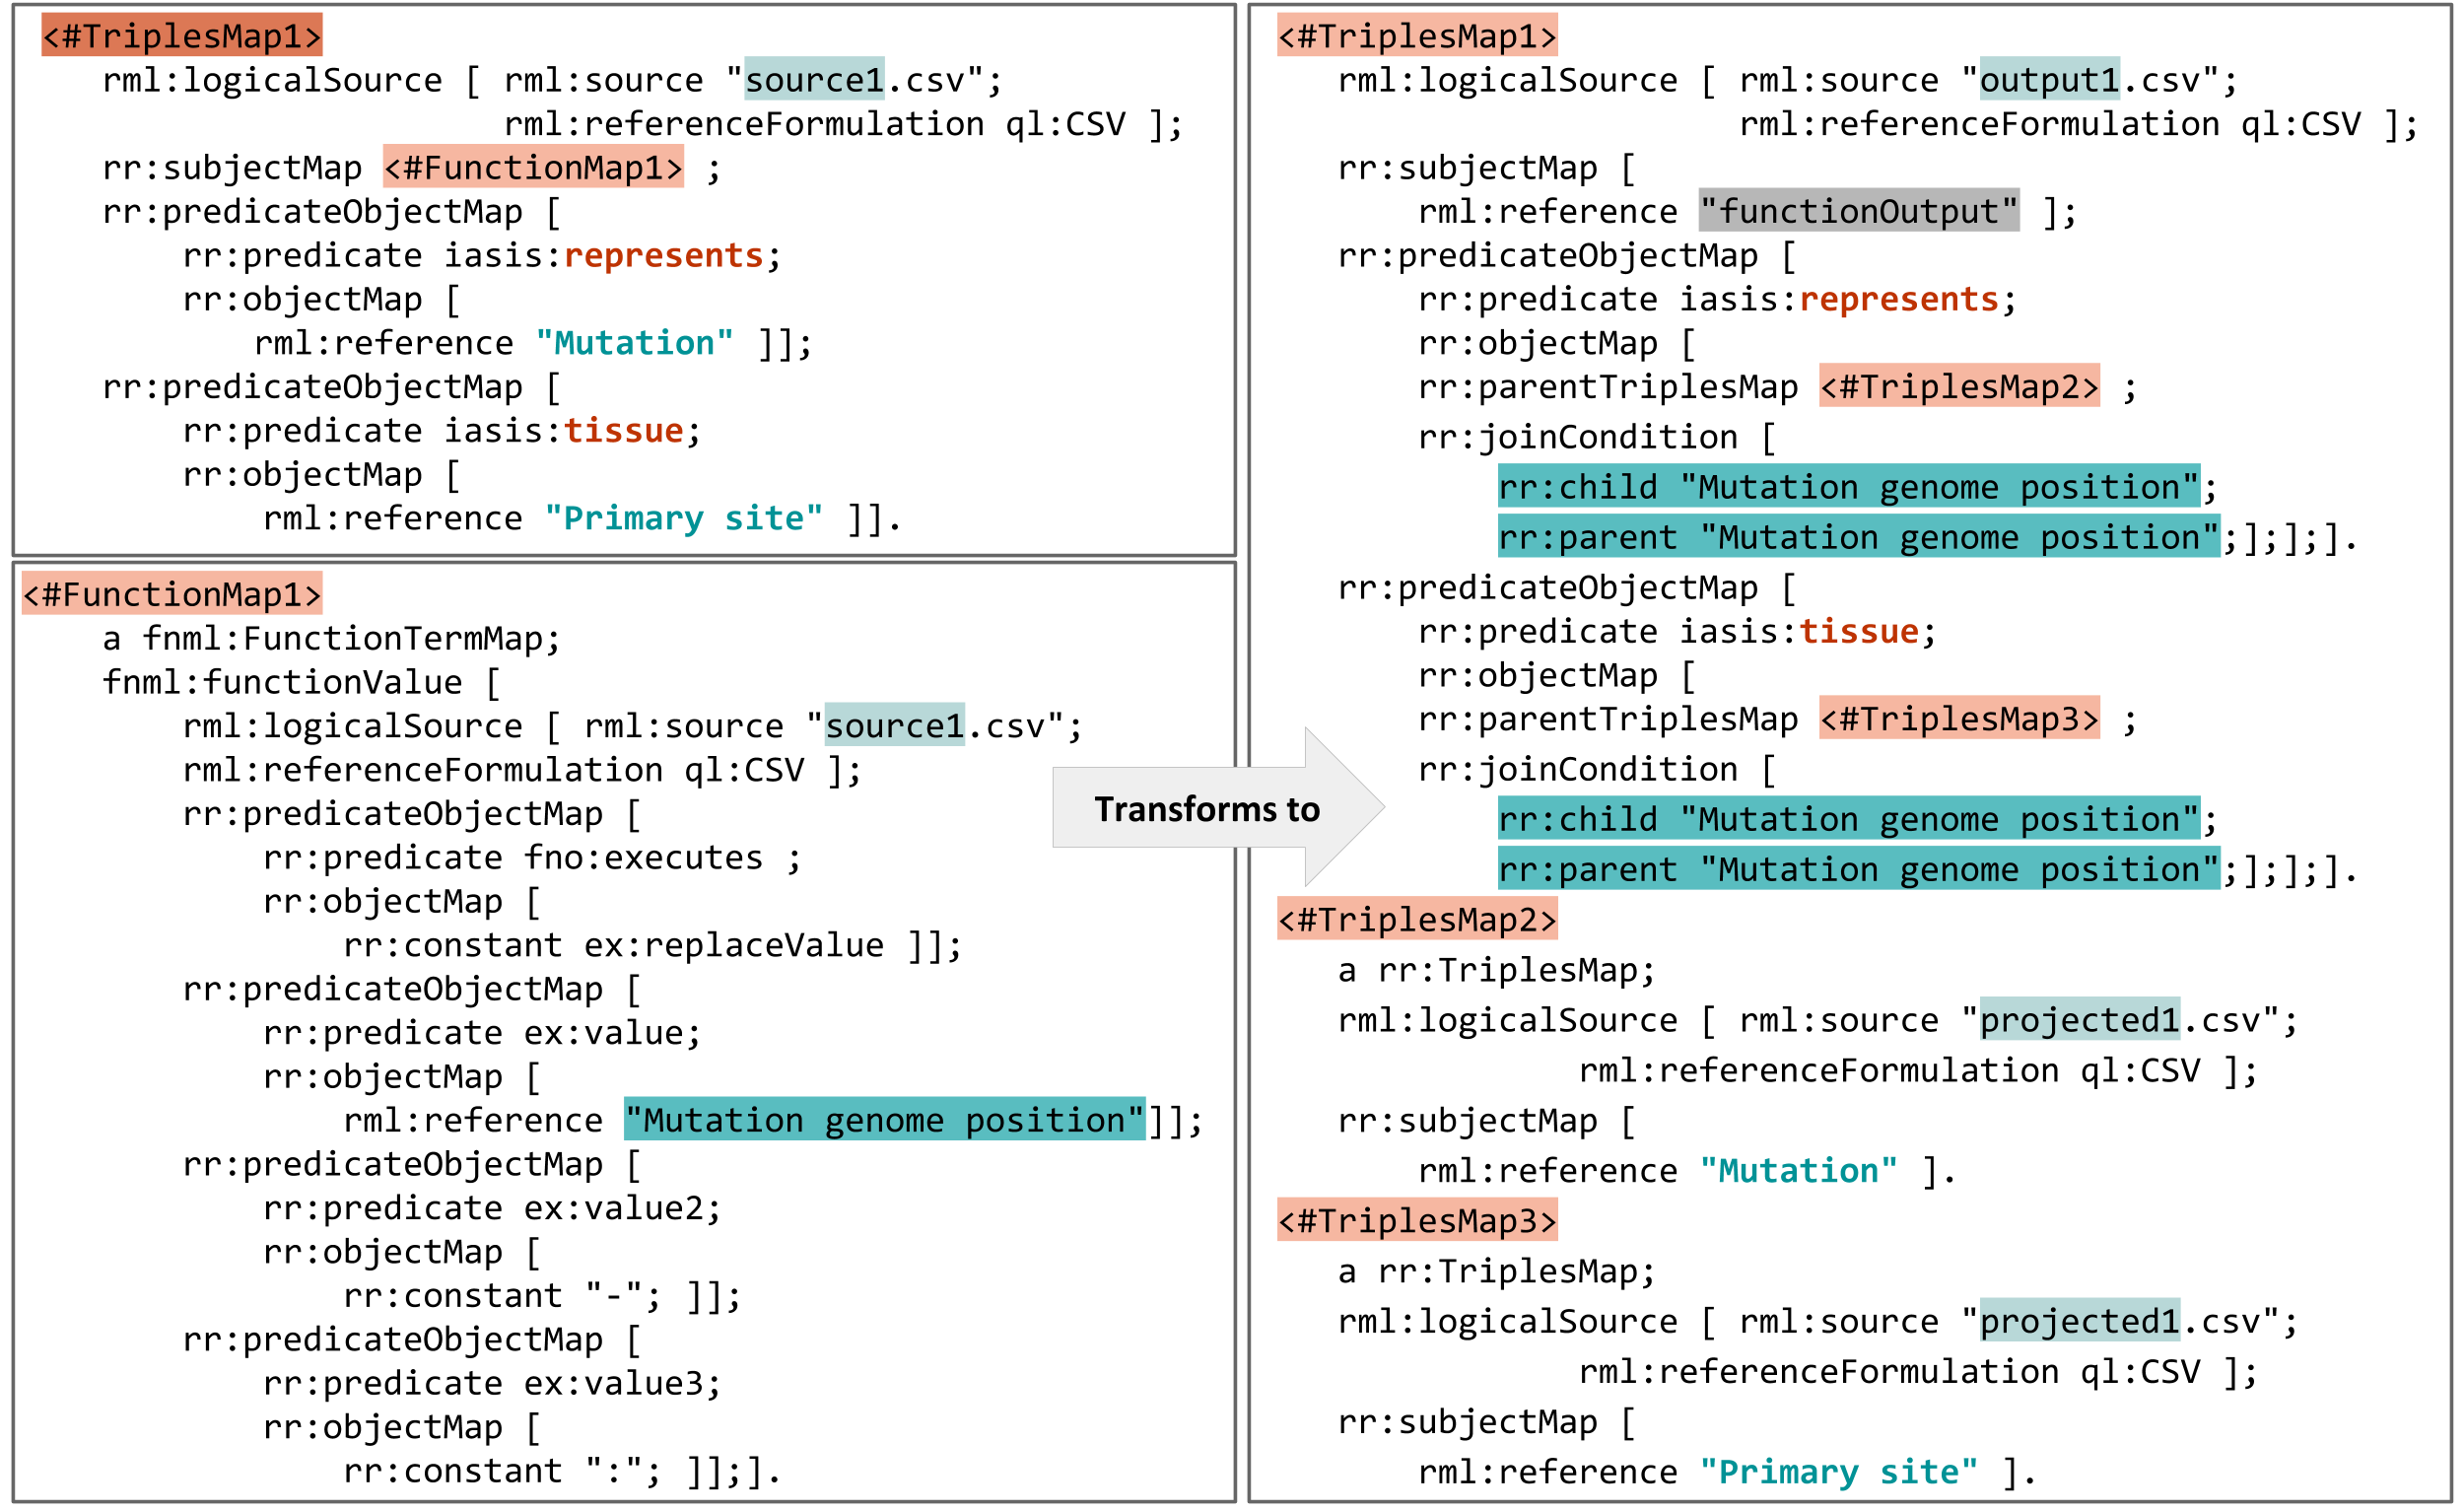
\includegraphics[width=\textwidth]{figures/MTR_subjectBased.png}
\caption[Example of Subject-based MTR]{\textbf{Example of Subject-based MTR.} An example of mappings including a TriplesMaps and FunctionMap are illustrated on the left and their transformed version including three TriplesMap are shown on the right side.} 
\label{fig:subjectBased}
\end{figure}
\noindent\textbf{Mapping Transformation Rules (MTRs)}
Mappings are transformed to create the same knowledge graph utilizing the transformed data sources. MTRs are defined considering the role of a transformation function $F_i$ in each \verb|TriplesMap| $T_i$.
I) $F_i$ as an \verb|ObjectMap|: 
We refer to the MTRs that are required in this case as \verb|Object-based|. First of all, for each $F_i$, a new \verb|TriplesMap| $T'_i$ is created; it refers to the data source generated as the outcome of $F_i$, i.e., $S_i^{output}$. Accordingly, the \verb|SubjectMap| of $T'_i$ refers to the output attributes $o_i$ in $S_i^{output}$. Afterwards, in \verb|TriplesMap| $T_i$ where $F_i$ is presented as an \verb|ObjectMap|, $F_i$ is replaced by a \verb|joinCondition| which joins $T_i$ and $T'_i$ over attributes $a'_i$, i.e., the input attributes of $F_i$. Moreover, the \verb|logicalSource| of $T_i$ is changed to $S_i
^{project}$, i.e., the corresponding projected data source provided as an outcome of DTR2. 
II) $F_i$ as a \verb|SubjectMap|: Contrary to the \verb|Object-based|, in this set of MTR - we refer to as \verb|Subject-based|- for each \verb|predicateObjectMap| that follows a $F_i$ of the type \verb|SubjectMap|, a new \verb|TriplesMap| $T'_i$ refers to the data source $S_i^{project}$ which is generated as an outcome of DTR2 by projecting the attribute $a'_i$ from $S_i$ that are referenced as \verb|objectMap| in the original \verb|predicateObjectMap|. The \verb|subjectMap| of $T'_k$ --the transformed $T_i$  -- refers to the $o_i$ and its \verb|logicalSource| is $S_i^{output}$.   
Note that \verb|subjectMap| of $T'_i$ is by definition a \verb|TermMap|, which means that its value can be any RDF term according to the RML specification.

Each \verb|objectMap| in $T_i$ that is a \verb|FunctionMap| is replaced by a \verb|joinCondition| between $T_i$ and corresponding $T'_i$ over input attributes $a'_i$ of $F_i$. 
In both cases, the transformed $T_i$-- denoted as $T'_k$-- and $T'_i$ are added to $M'$ and $T_i$ is removed from $M'$. \\     
Figures \ref{fig:objectBased} and \ref{fig:subjectBased} illustrate two examples of rewritten mappings based on DTRs and MTRs. In the left side of both figures, the original mappings are presented while the transformed mappings are depicted on the right side. In the transformed mappings in \autoref{fig:objectBased}, \verb|TriplesMap3| is created for \verb|FunctionMap1|; it refers to the attribute \verb|functionOutput| in the projected data source \verb|output1.csv|-- shown in \autoref{fig:funmap-dtr}.c. Then, \verb|FunctionMap1| is replaced in both \verb|TriplesMap1| and \verb|TriplesMap2| by a join condition over the attribute \verb|Mutation genome position| which is the input attribute of \verb|FunctionMap| in the original mapping file as it is highlighted by the same \textcolor{metallicSeaweed}{\textbf{color}}. Accordingly, data sources -\textcolor{powderBlue}{\textbf{highlighted}}- of \verb|TriplesMap|s are also transformed to refer to the projected data sources. 
Consider \autoref{fig:subjectBased} where \verb|FunctionMap| is a \verb|subjectMap|. In both \verb|predicateObjectMa|-\verb|p|s of \verb|TriplesMap1|, \verb|FunctionMap1| is replaced by a \verb|joinCondition| over the attribute \verb|Mutation genome position| that is the input of \verb|FunctionMap1|. To better clarify the performed transformation, consider the first \verb|predicateObjectMap| in \verb|TripleMap1| in the original mappings; the \verb|predicate| is \textcolor{burntSienna}{\textbf{represents}} and the \verb|ObjectMap| refers to the attribute \textcolor{metallicSeaweed}{\textbf{Mutation}}. After the transformation, the first \verb|predicateObjectMap| has the same \verb|predicate| \textcolor{burntSienna}{\textbf{represents}} and through the \verb|joinCondition| refers to the same attribute \textcolor{metallicSeaweed}{\textbf{Mutation}} in \verb|projected1.csv|. 

\subsubsection{Lossless Transformation Rules}
\label{subsec:formalEval}
We validated the correctness of the transformations that are performed by FunMap, by proving that the RDF triples produced by $DIS'_G$ are identical to the ones generated by $DIS_G$.

Consider:
\begin{itemize}
    \item The Ontology $O$ is defined as a triple, $O=(C,P,Axioms)$ where $C$ and $P$ represent the classes and properties of $O$ respectively. The $Axioms$ stands for a set of statements expressing the characteristics of the properties of $O$.  
    \item The data sources of $DIS_G$ are defined as a set of $S_j^{A_j}$ where $S_j$ stands for a data source and $A_j$ represents attributes of $S_j$ that are utilized by $M$.
    \item The $M$ describing the classes $C$ and properties $P$ in $O$ in terms of sources in $S$ comprises a set of mapping rule $r_i$ that is defined as:
        \[r_i :  c_j(X,\overline{X}) : - S_1(\overline{X_1}), S_2(\overline{X_2}),\dots, S_m(\overline{X_m}) \]
    Where $c_j$ is a class in $C$, $X$ is a variable, and $\overline{X}$ is a set of pairs , and $X_{i,j}$ is a variable. The predicate $S_z(\overline{X_z})$ represents a source $S_z$ in $S$ and $\overline{X_z}$ is a set of pairs $(a_{i,z},X_{i,z})$ where $X_{i,z}$ is a variable and $att_{i,z}$ is an attribute of $S_z$. 
\end{itemize}
For each mapping rule in $M$ with sources $S_z(\overline{X_z})$ and a set of utilized attributes as $\prod_{att}S_z$, DTR1 and DTR2 add new sources $S_y(\overline{X_y})$ and $S_w(\overline{X_w})$ in the way that $\prod_{att}S_y$ + $\prod_{att}S_w$ equals $\prod_{att}S_z$. Accordingly, for each mapping rule in $M$:
\begin{itemize}
    \item If a mapping includes \verb|FunctionMap| in \verb|ObjectMap|:\\
    $(att_{A,z},X_{sub,z})+(att_{f(B),z},X_{obj,z})$ =? 
    $(att_{A,w},X_{sub,w})+(att_{B,w},X_{join,w})+(att_{B,y
    },X_{join,y})+(att_{f(B),y},X_{obj,y})$
\end{itemize}


Pre- and post-conditions of Data Source Transformation Rules (DTRs) and Mapping Transformation Rules (MTRs) are stated in the following properties:
\noindent\textit{Property 1.}(Lossless Function)
\label{property:p1}
Given data integration systems $DIS_G$=$\langle O,S,M \rangle$ and  $DIS_G'$=$\langle O,S',M \rangle$ such that $DIS_G'$ is the result of applying one DTR1 transformation to $DIS_G$. Then, there are data sources $S_i$ and 
$S_i^{output}$ in $S$ and $S'$, respectively, and the following statements hold:
\begin{itemize}
    \item $S'- S=\{S_i^{output}\}$, there is a mapping $T_i$ in $M$ with a function $F_i$, and \textit{Attrs} contains the attributes $a'_i$ of $F_i$ in $S_i$ and the output attributes $o_i$ of $F_i$. 
    \item  $S_i^{output}$ comprises the attributes \textit{Attrs} and $\pi_{a'_i}(S_i^{output})$=$\pi_{a'_i}(S_i)$.  
    \item For each tuple $t_{i,j}$ in $S_i^{output}$, the values of the attributes $o_i$ in $t_{i,j}$ correspond to the result of $F_i$ over the values of $a'_i$ in $t_{i,j}$, i.e., $t_{i,j}.o_i$=$F_i(t_{i,j}.a'_i)$. 
    
\end{itemize}


\noindent\textit{Property 2.}(Lossless Projection)
\label{property:p2}
Given data integration systems $DIS_G$=$\langle O,S,M \rangle$ and  $DIS_G'$=$\langle O,S',M \rangle$ such that $DIS_G'$ is the result of applying one DTR2 transformation to $DIS_G$. Then, there are data sources $S_i$ 
and $S_i^{project}$ in $S$ and $S'$, respectively, and the following statements hold:
\begin{itemize}
    \item $S'- S=\{S_i^{project}\}$, and there is a mapping $T_i$ in $M$ defined over the attributes \textit{Attrs} from $S_i$, and $S_i^{project}=\pi_{\textit{Attrs}}(S_i)$. 
\end{itemize}


\noindent\textit{Property 3.} (Lossless Schema-Ontology Alignments)\footnote{Similarly, this property can be stated for the result of applying MTR over the subject position of a property in a mapping of a data integration system.}
\label{property:p3}
Given data integration systems $DIS_G$=$\langle O,S,M\rangle$ and  $DIS_G'$=$\langle O,S,M'\rangle$ such that $DIS_G'$ is the result of applying one MTR transformation to $DIS_G$. Then, there are \verb|TriplesMap|s $T_i$ in $M$, 
and  $T'_i$ and $T'_k$ in $M'$, and the following statements hold:
\begin{itemize}
    \item $M - M'=\{T_i\}$ and $M'- M=\{T'_i,T'_k\}$. 
    \item There is a function $F_i$ in $T_i$ as the \verb|ObjectMap| of a  \verb|PredicateMap| $p$, and there is a data source $S_i^{output}$ in $S$ which is the \verb|LogicalSource| of $T_i$. The attributes of $S_i^{output}$ are the union of $a'_i$ and $o_i$, while $a'_i$ and $o_i$ are input and output attributes of $F_i$, respectively.
    \item $T_i$ and $T'_k$ are defined over the same \verb|LogicalSource|  $S_i^{project}$. $S_i^{output}$ is the \verb|LogicalSource| of $T'_i$ and $o_i$ is the \verb|SubjectMap| of $T'_i$.  
    \item $T_i$ and $T'_k$ only differ on the \verb|ObjectMap| $p$. In $T_i$, \verb|ObjectMap| of $p$ is defined as $F_i$, while in $T'_k$, a \verb|joinCondition| to $T'_i$ on $a'_i$ defines the \verb|ObjectMap| of $p$. 
\end{itemize}


\subsection{Experimental Evaluation}

In this section, we evaluate FunMap\footnote{\url{https://doi.org/10.5281/zenodo.3993657}} in comparison to current approaches that create a knowledge graph using the specified data sources and RML+FnO mappings. Following the hypothesis H5 defined in Chapter \ref{chap:objectives}, we aim to answer the following research questions: 
\textbf{R1:} What is the impact of data duplication rate in the execution time of a knowledge graph creation approach?; \textbf{RQ2:} What is the impact of different types of complexity over transformation functions during a knowledge graph creation process?; \textbf{Q3:} How does the repetition of a same function in different mappings affect the existing RML engines?; \textbf{Q4:} What is the impact of relational data sources in the knowledge graph creation process?
All the resources used to perform this evaluation are available in our Github repository\footnote{\url{https://github.com/SDM-TIB/FunMap}}. The experimental configuration is as follows:

\noindent\textbf{Datasets and Mappings.}
To the best of our knowledge, there are no testbeds to evaluate the performance of a knowledge graph construction approach that applies functional mappings. Consequently, following the real-world scenario that initially motivated this research, we create our testbed from the biomedical domain. We generate a baseline dataset by randomly selecting 20,000 records from the coding point mutation dataset in COSMIC\footnote{\url{https://cancer.sanger.ac.uk/cosmic} GRCh37, version90, released August 2019} database. We keep all 39 attributes of the original dataset in the baseline dataset, while only five to seven of them are utilized in mappings. In total, four different mapping files are generated consisting of one \verb|FunctionMap| and four, six, eight, or ten \verb|TriplesMap|s with a \verb|predicateObjectMap| linked to the function. To additionally validate FunMap in case of large-sized data, we create another dataset following the same criteria, with 4,000,000 records and the size of about 1.3GB.

\noindent\textbf{Engines.}
The baselines of our study are three different open source RML-complaint engines that are able to execute RML+FnO mappings and have been extensively utilized in multiple applications and tested by the community: SDM-RDFizer v3.0~\citep{iglesias2020sdm}, RMLMapper\footnote{\url{https://github.com/RMLio/rmlmapper-java}} v4.7, and RocketRML v1.6~\citep{csimcsek2019rocketrml}\footnote{We name them SDM-RDFizer**(RML+FnO), RMLMapper**(RML+FnO), and RocketRML**(RML+FnO).}. In order to evaluate the impact of transformation rules, we implement FunMap v1.0 on the top of the aforementioned engines with DTR2 optimization as an optional parameter. We refer to the approach which applies FunMap excluding DTR2 as FunMap$^-$\footnote{We name these combined engines as follows: a) FunMap: FunMap+SDM-RDFizer, FunMap+RMLMapper, and FunMap+RocketRML; b) FunMap$^-$: FunMap$^-$+SDM-RDFizer, FunMap$^-$+RMLMapper, and FunMap$^-$+RocketRML.}. We created a docker image per tested engine for reproducibility.  

\noindent\textbf{Metrics.} \textit{Execution time:} Elapsed time spent by an engine to complete the creation of a knowledge graph and also counts FunMap pre-processing; it is measured as the absolute wall-clock system time as reported by the \verb|time| command of the Linux operating system. Each experiment was executed five times and average is reported. The experiments were executed on an Ubuntu 16.04 machine with Intel(R) Xeon(R) Platinum 8160, CPU 2.10GHz and 700Gb RAM. 

\noindent\textbf{Experimental setups.} Based on our research questions, we set up in overall 198 experiments as the combinations of the following scenarios. We create two datasets from our baseline with 25\% and 75\% duplicates which means in the 25\% duplicate dataset, 25\% and in the 75\% duplicate dataset, 75\% of the records are duplicated. Additionally, two functions with different levels of complexity are created. We describe the complexity level of the functions based on the number of required input attributes and operations to be performed. Accordingly, ``simple'' function is defined to receive one input attribute and perform one operation, while a ``complex'' function receives two input attributes and completes five operations. In total, we create eight mapping files including four, six, eight, and ten \verb|TriplesMap| and one \verb|FunctionMap| to be either ``simple'' or  ``complex''. Additionally, six experiments using 75\% duplicate datasets of 20,000 and 4,000,000 records and a mapping file including ten complex functions are set up in order to be run over a relational database (RDB) implemented in MySQL 8.0 \footnote{https://www.mysql.com/}.   

 \begin{figure}[t!]
 \centering
    \subfloat[SDM-RDFizer - 25\% of duplicates]{
        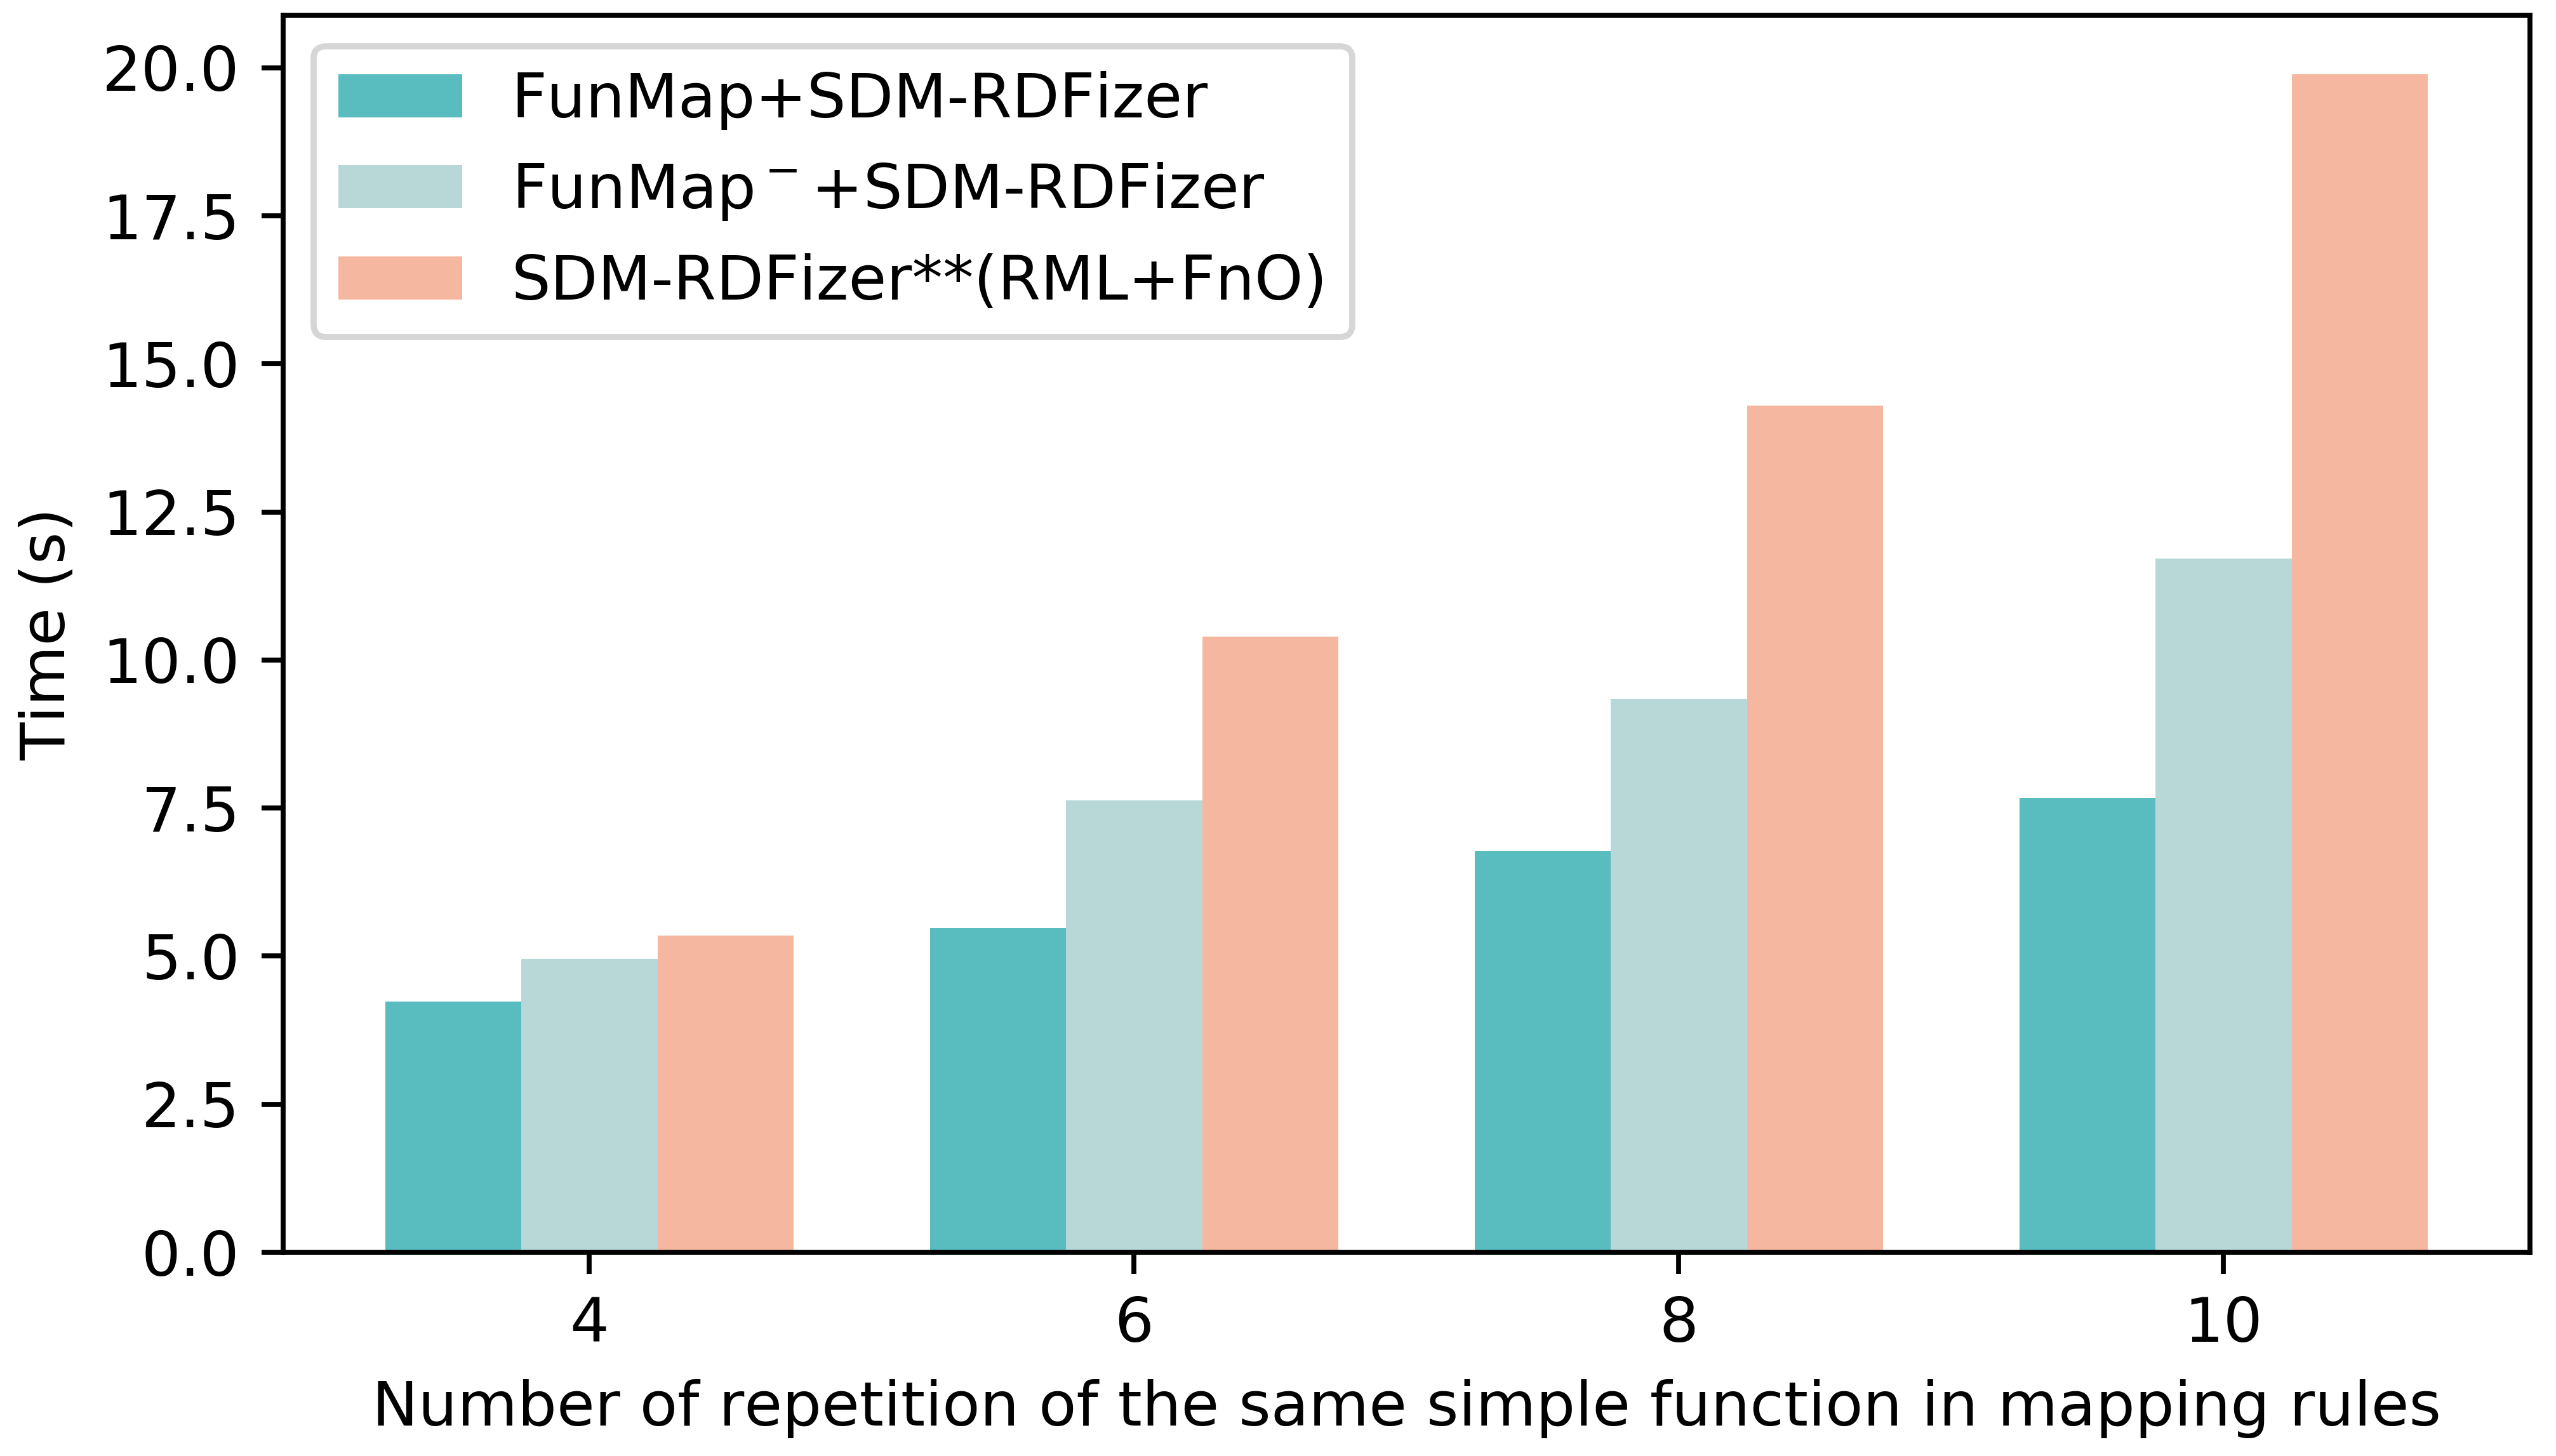
\includegraphics[width=0.46\columnwidth]{figures/veracity25_sdmrdfizer_simple.png}
            \label{fig:vera25_sdmrdfizer}}
    \subfloat[SDM-RDFizer - 75\% of duplicates]{
        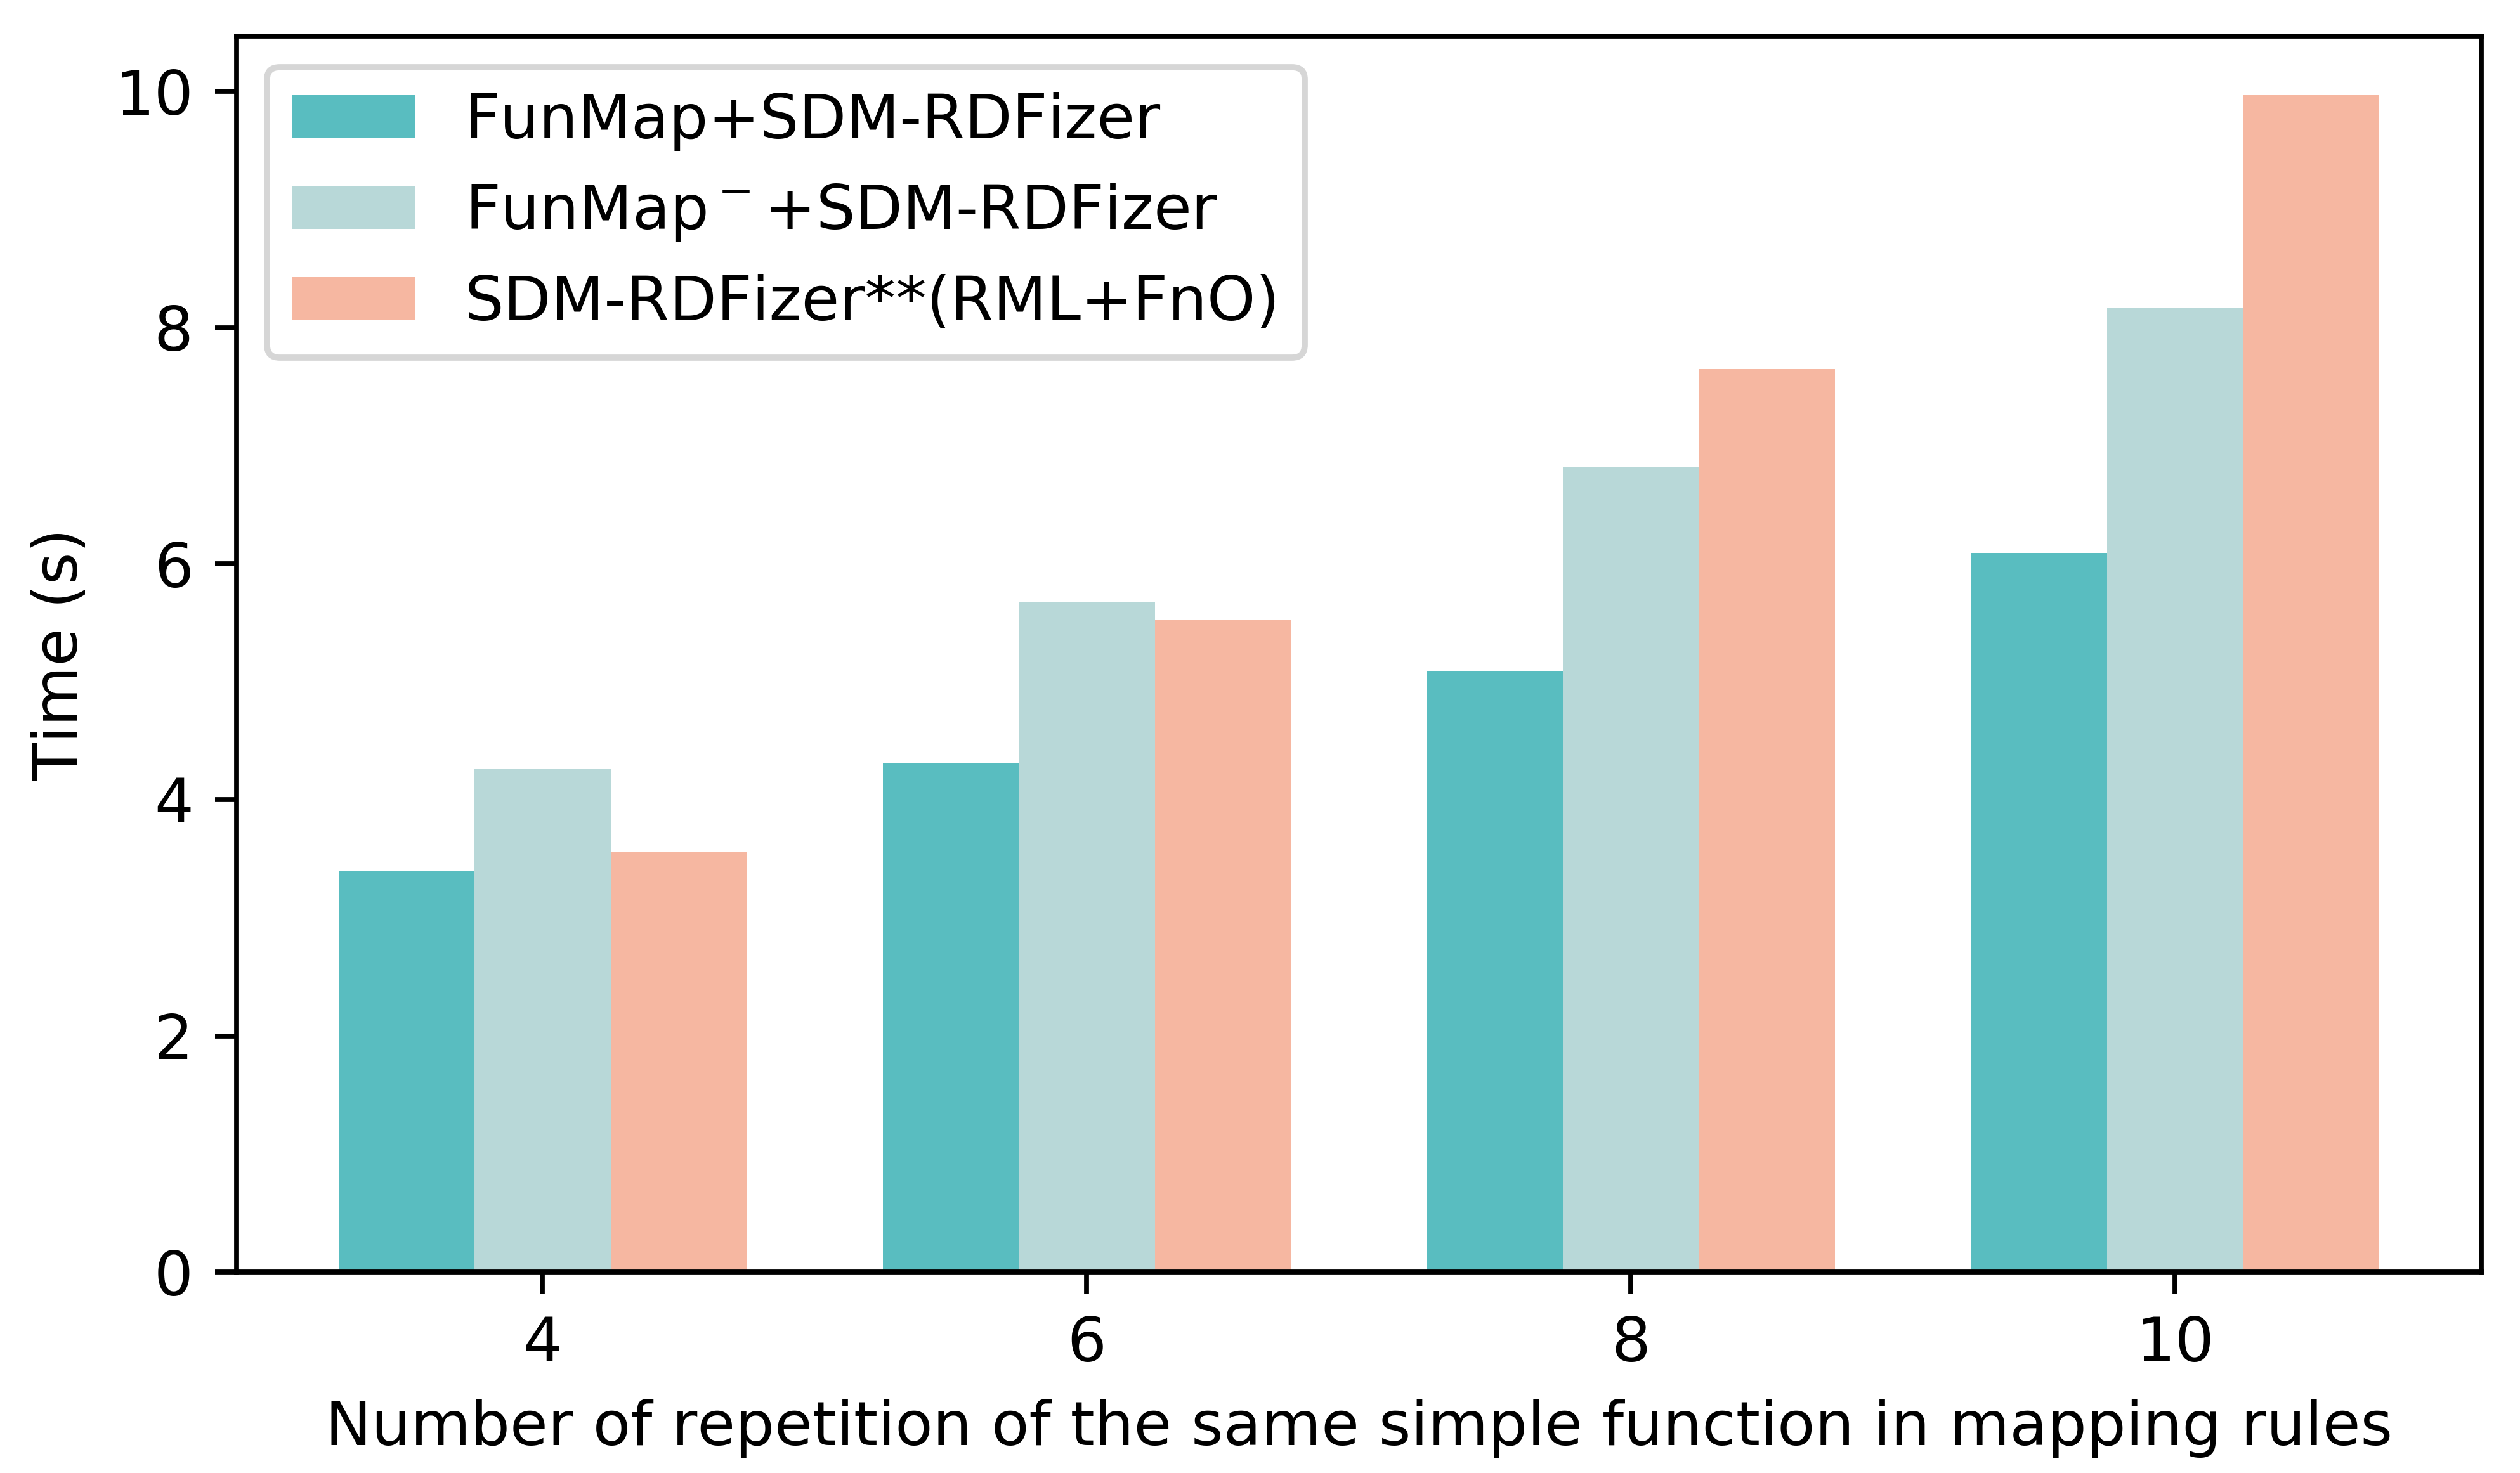
\includegraphics[width=0.45\columnwidth]{figures/veracity75_sdmrdfizer_simple.png}
            \label{fig:vera75_sdmrdfizer}}
\\            
    \subfloat[RMLMapper - 25\% of duplicates]{
        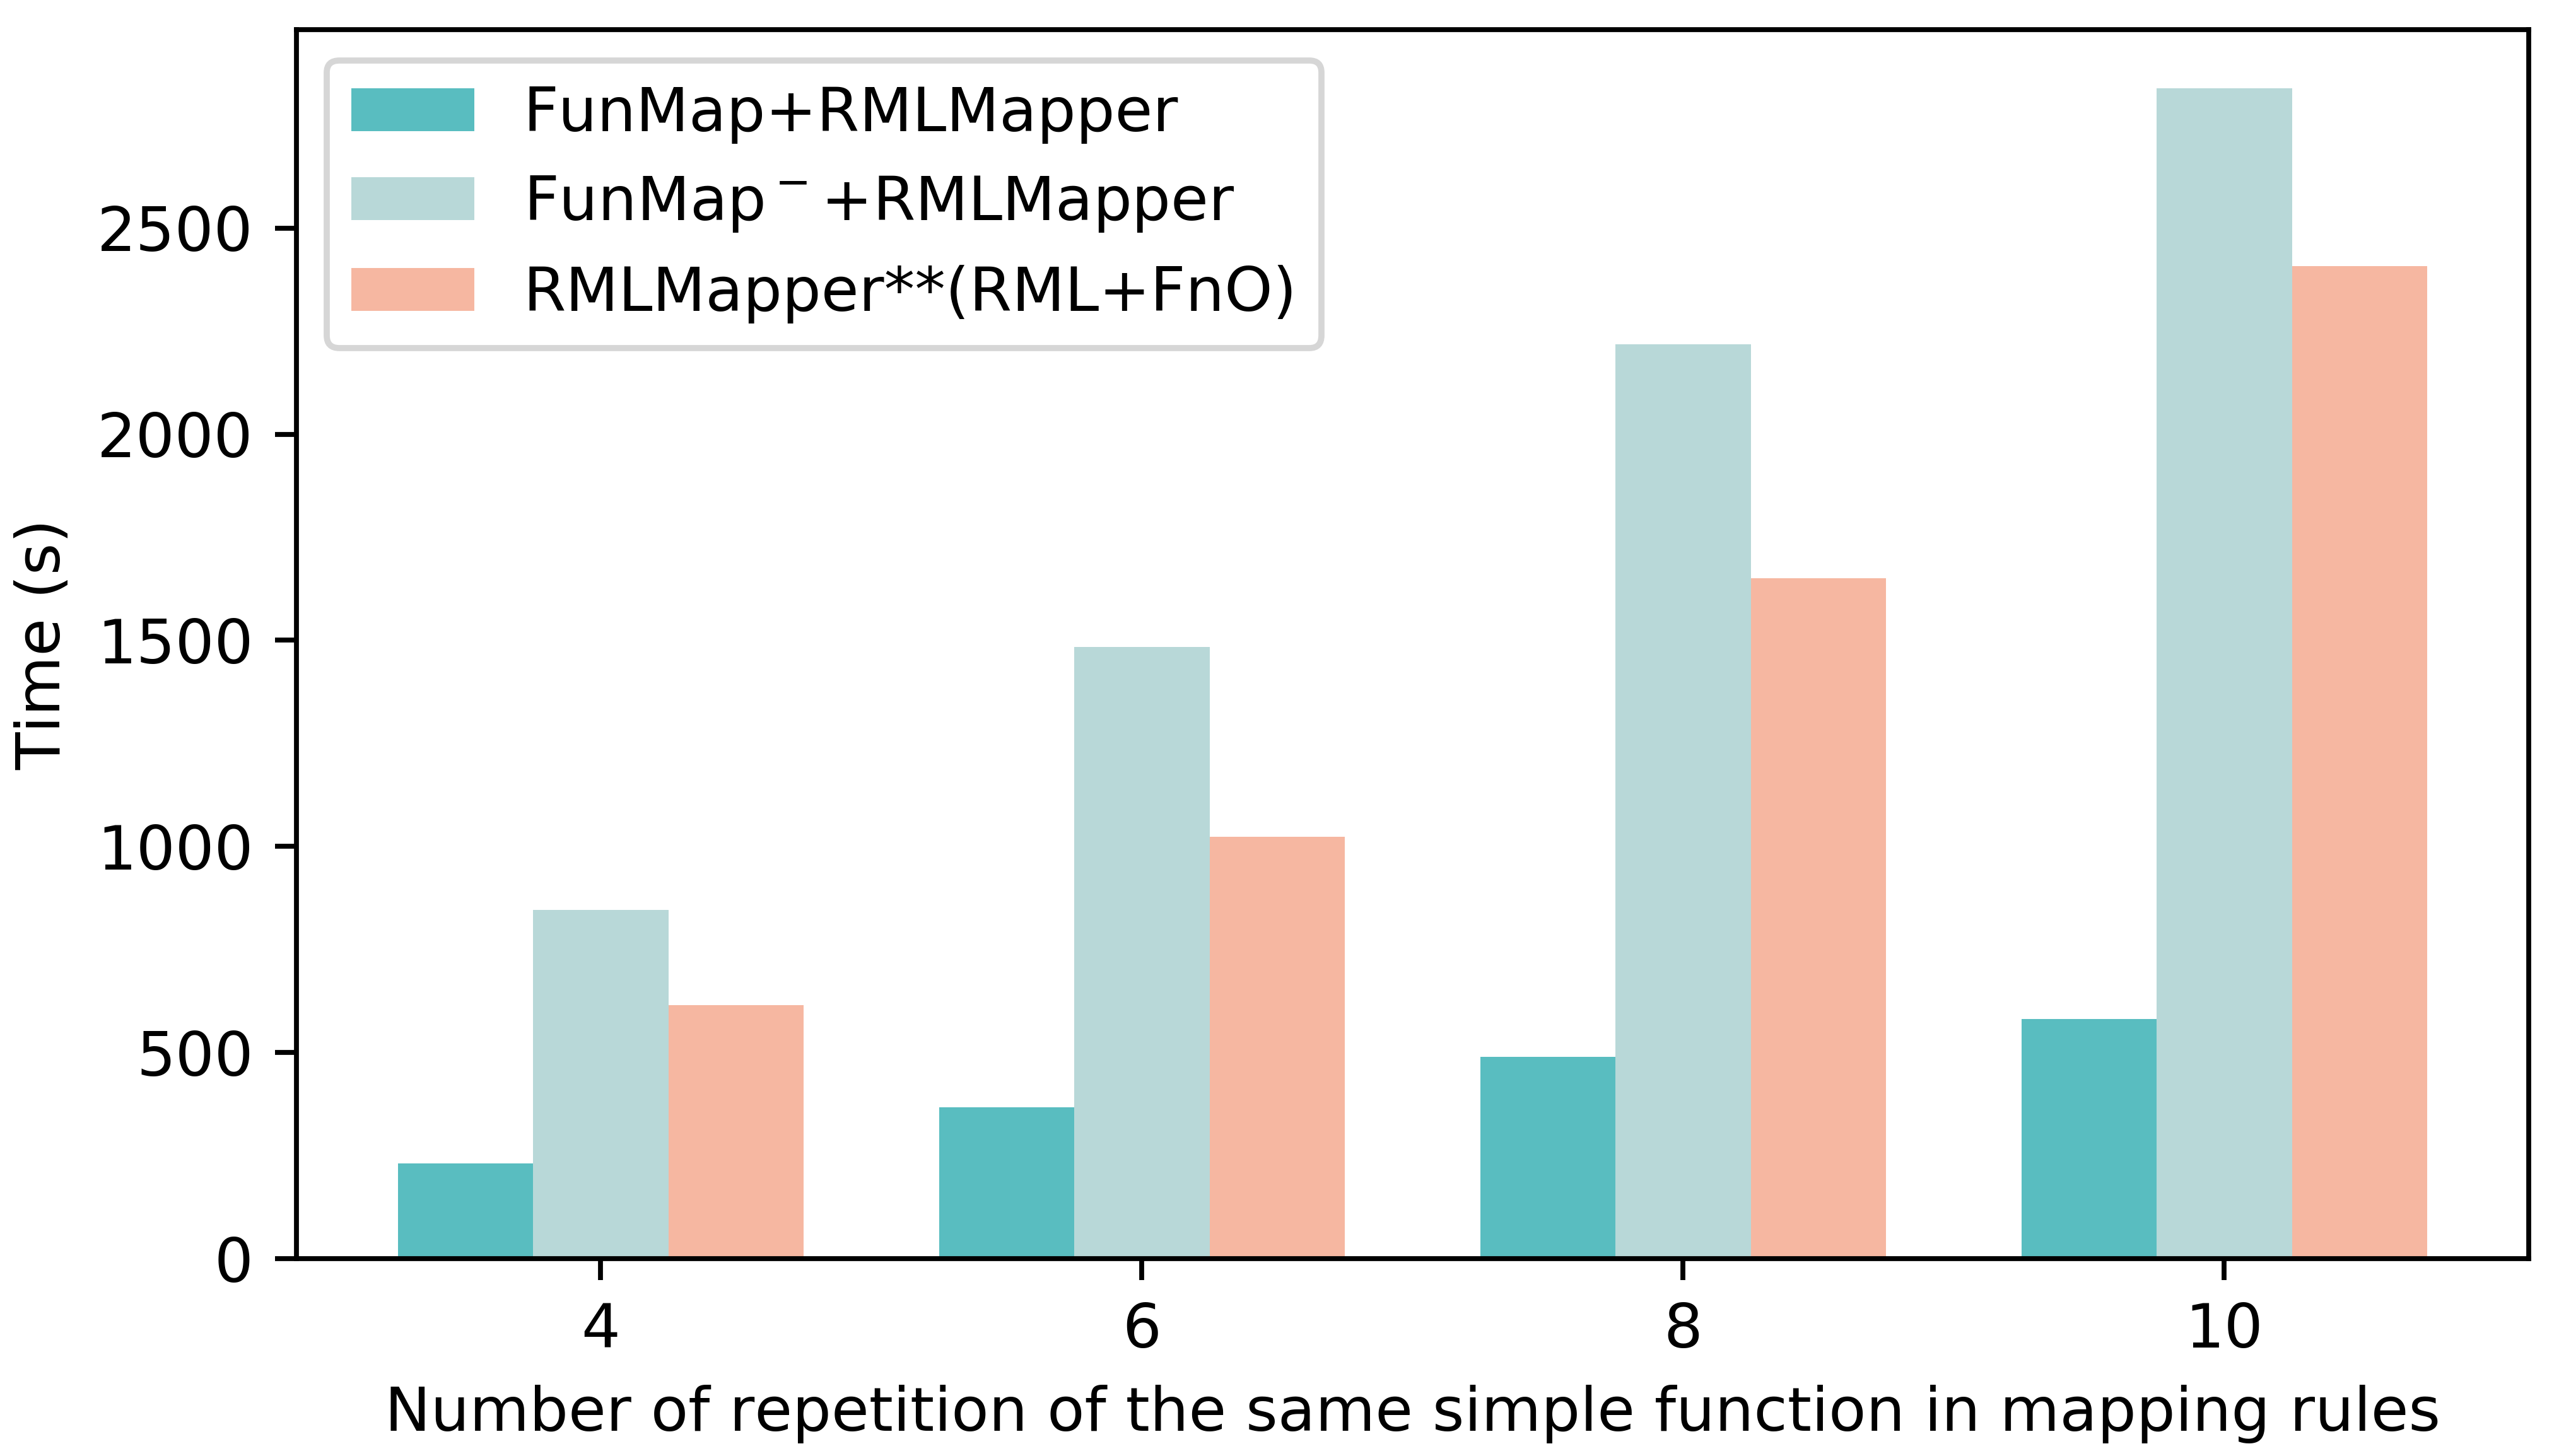
\includegraphics[width=0.45\columnwidth]{figures/veracity25_rmlmapper_simple.png}
            \label{fig:vera25_rmlmapper}}  
    \subfloat[RMLMapper - 75\% of duplicates]{
        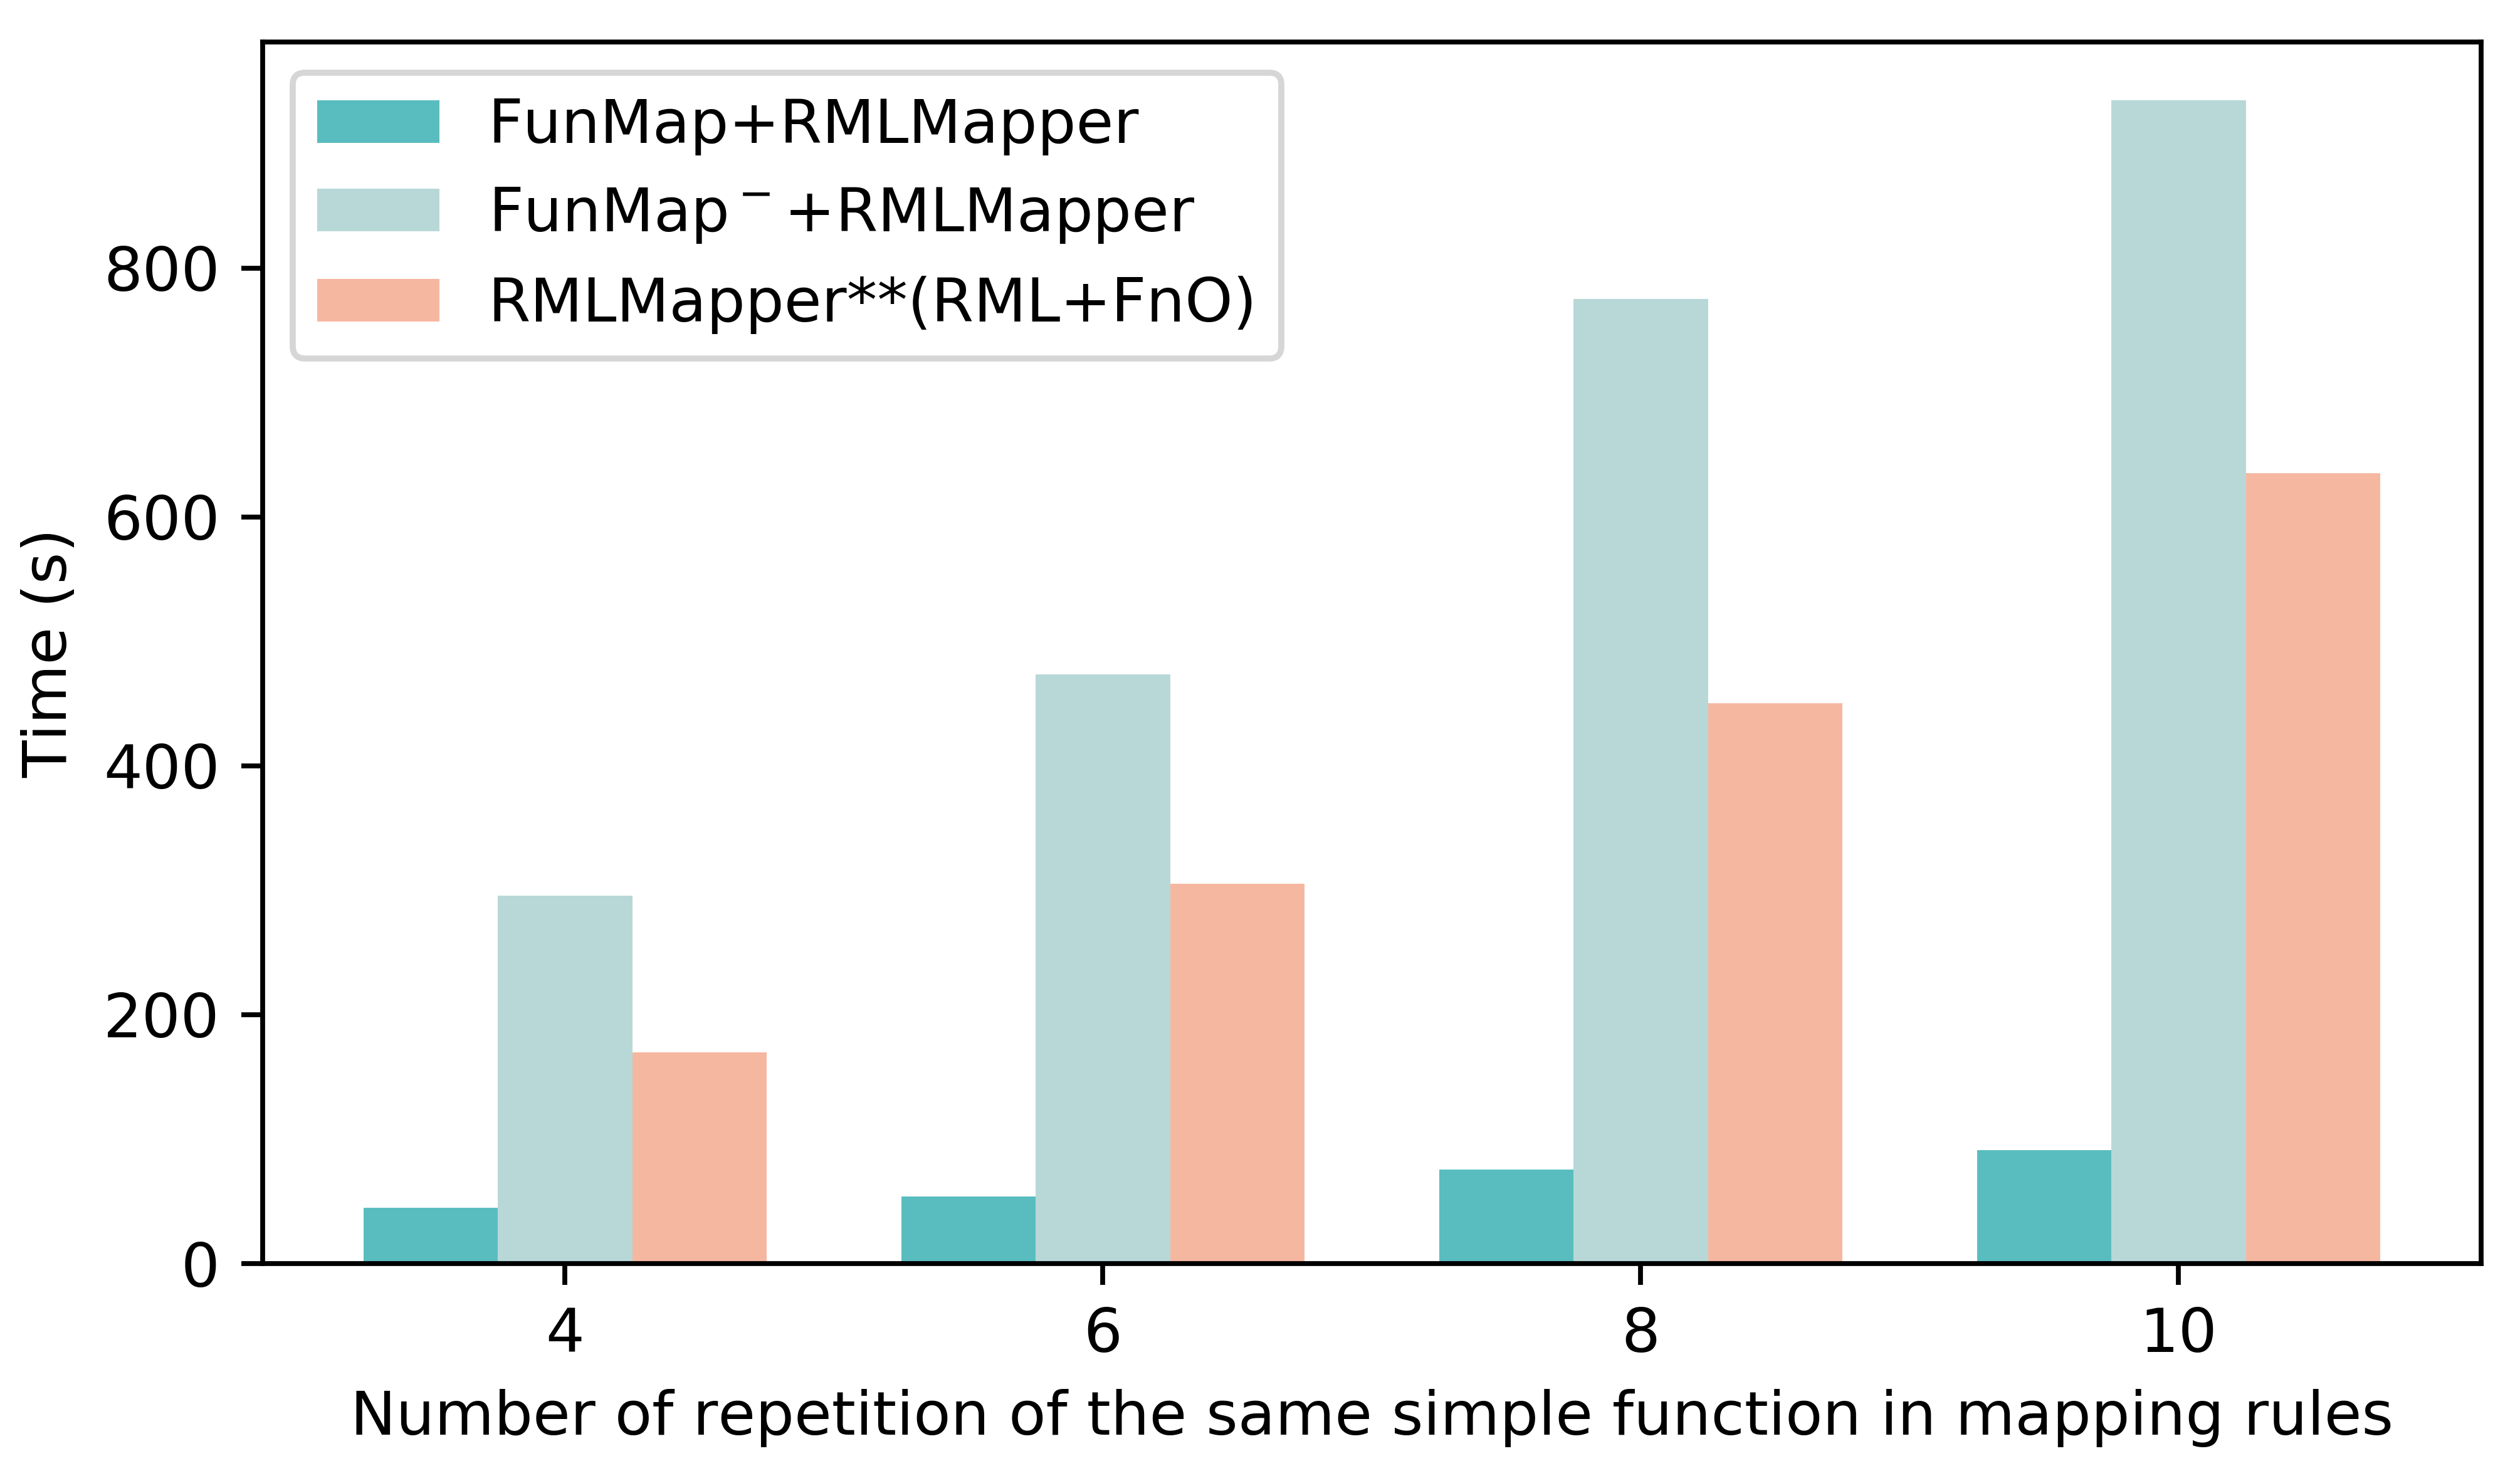
\includegraphics[width=0.45\columnwidth]{figures/veracity75_rmlmapper_simple.png}
            \label{fig:vera75_rmlmapper}} 
\\
    \subfloat[RocketRML - 25\% of duplicates]{
        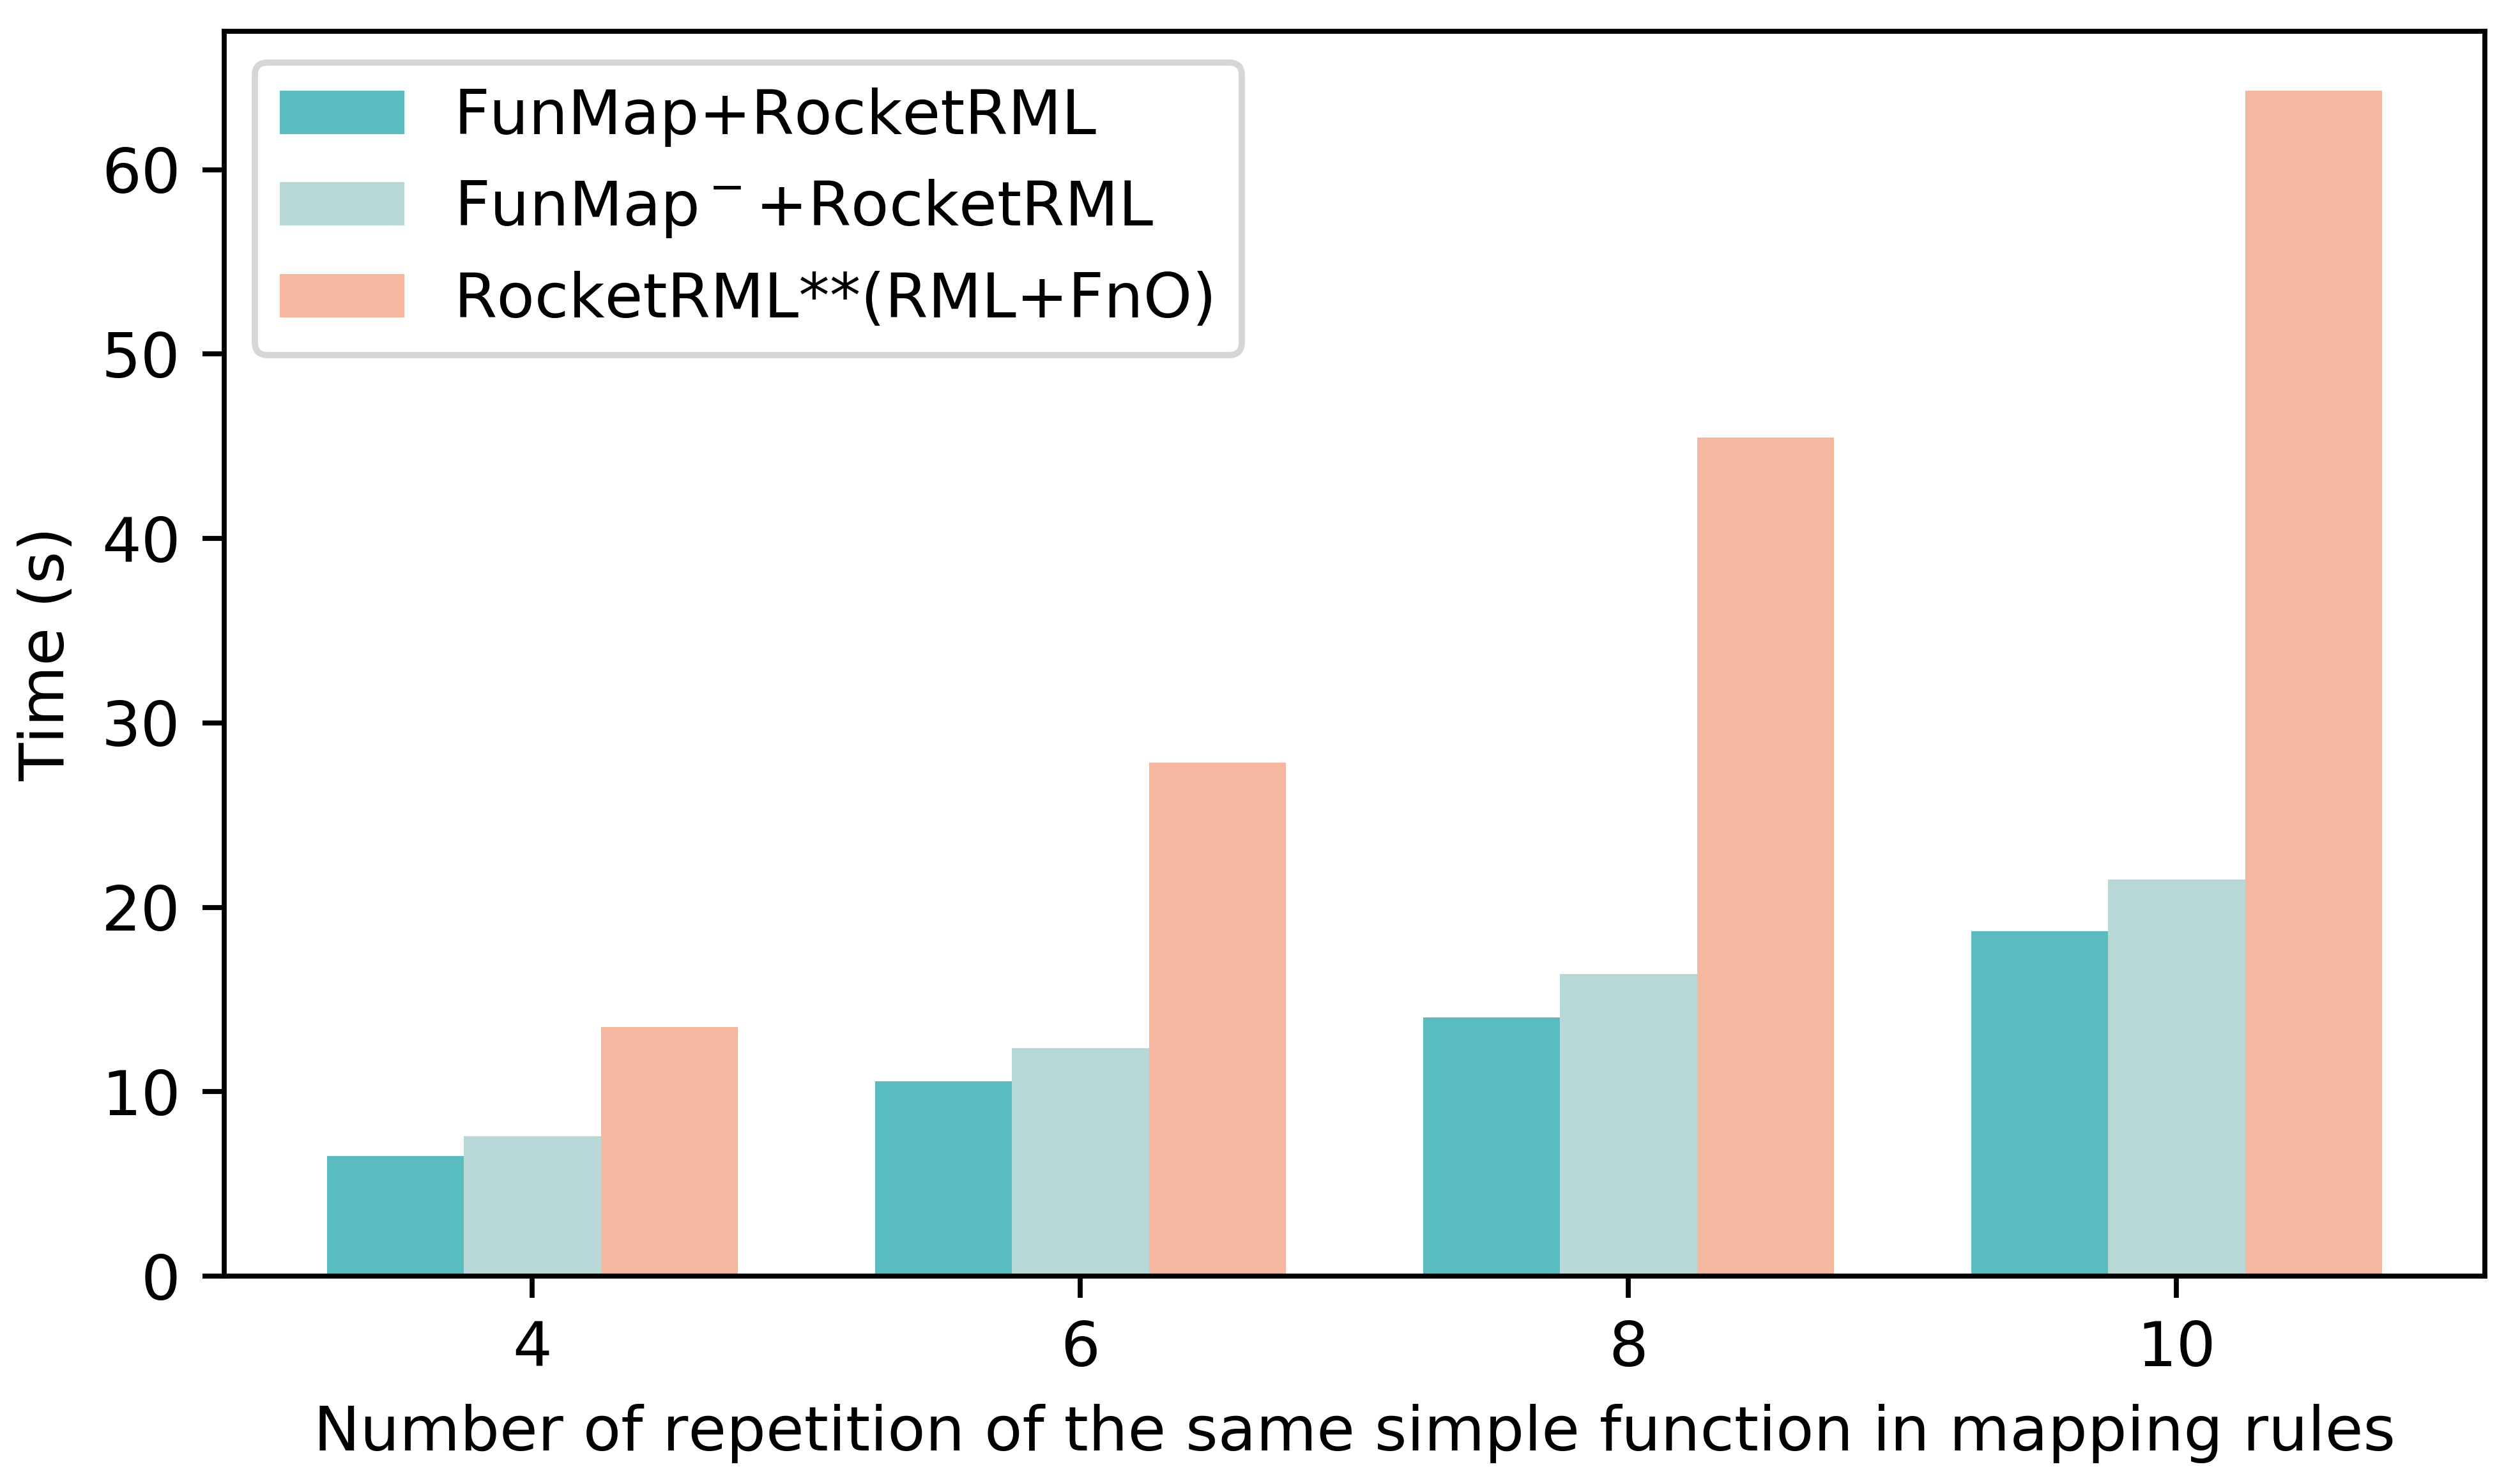
\includegraphics[width=0.45\columnwidth]{figures/veracity25_rocketrml.png}
            \label{fig:vera25_rocketrml}}
    \subfloat[RocketRML - 75\% of duplicates]{
        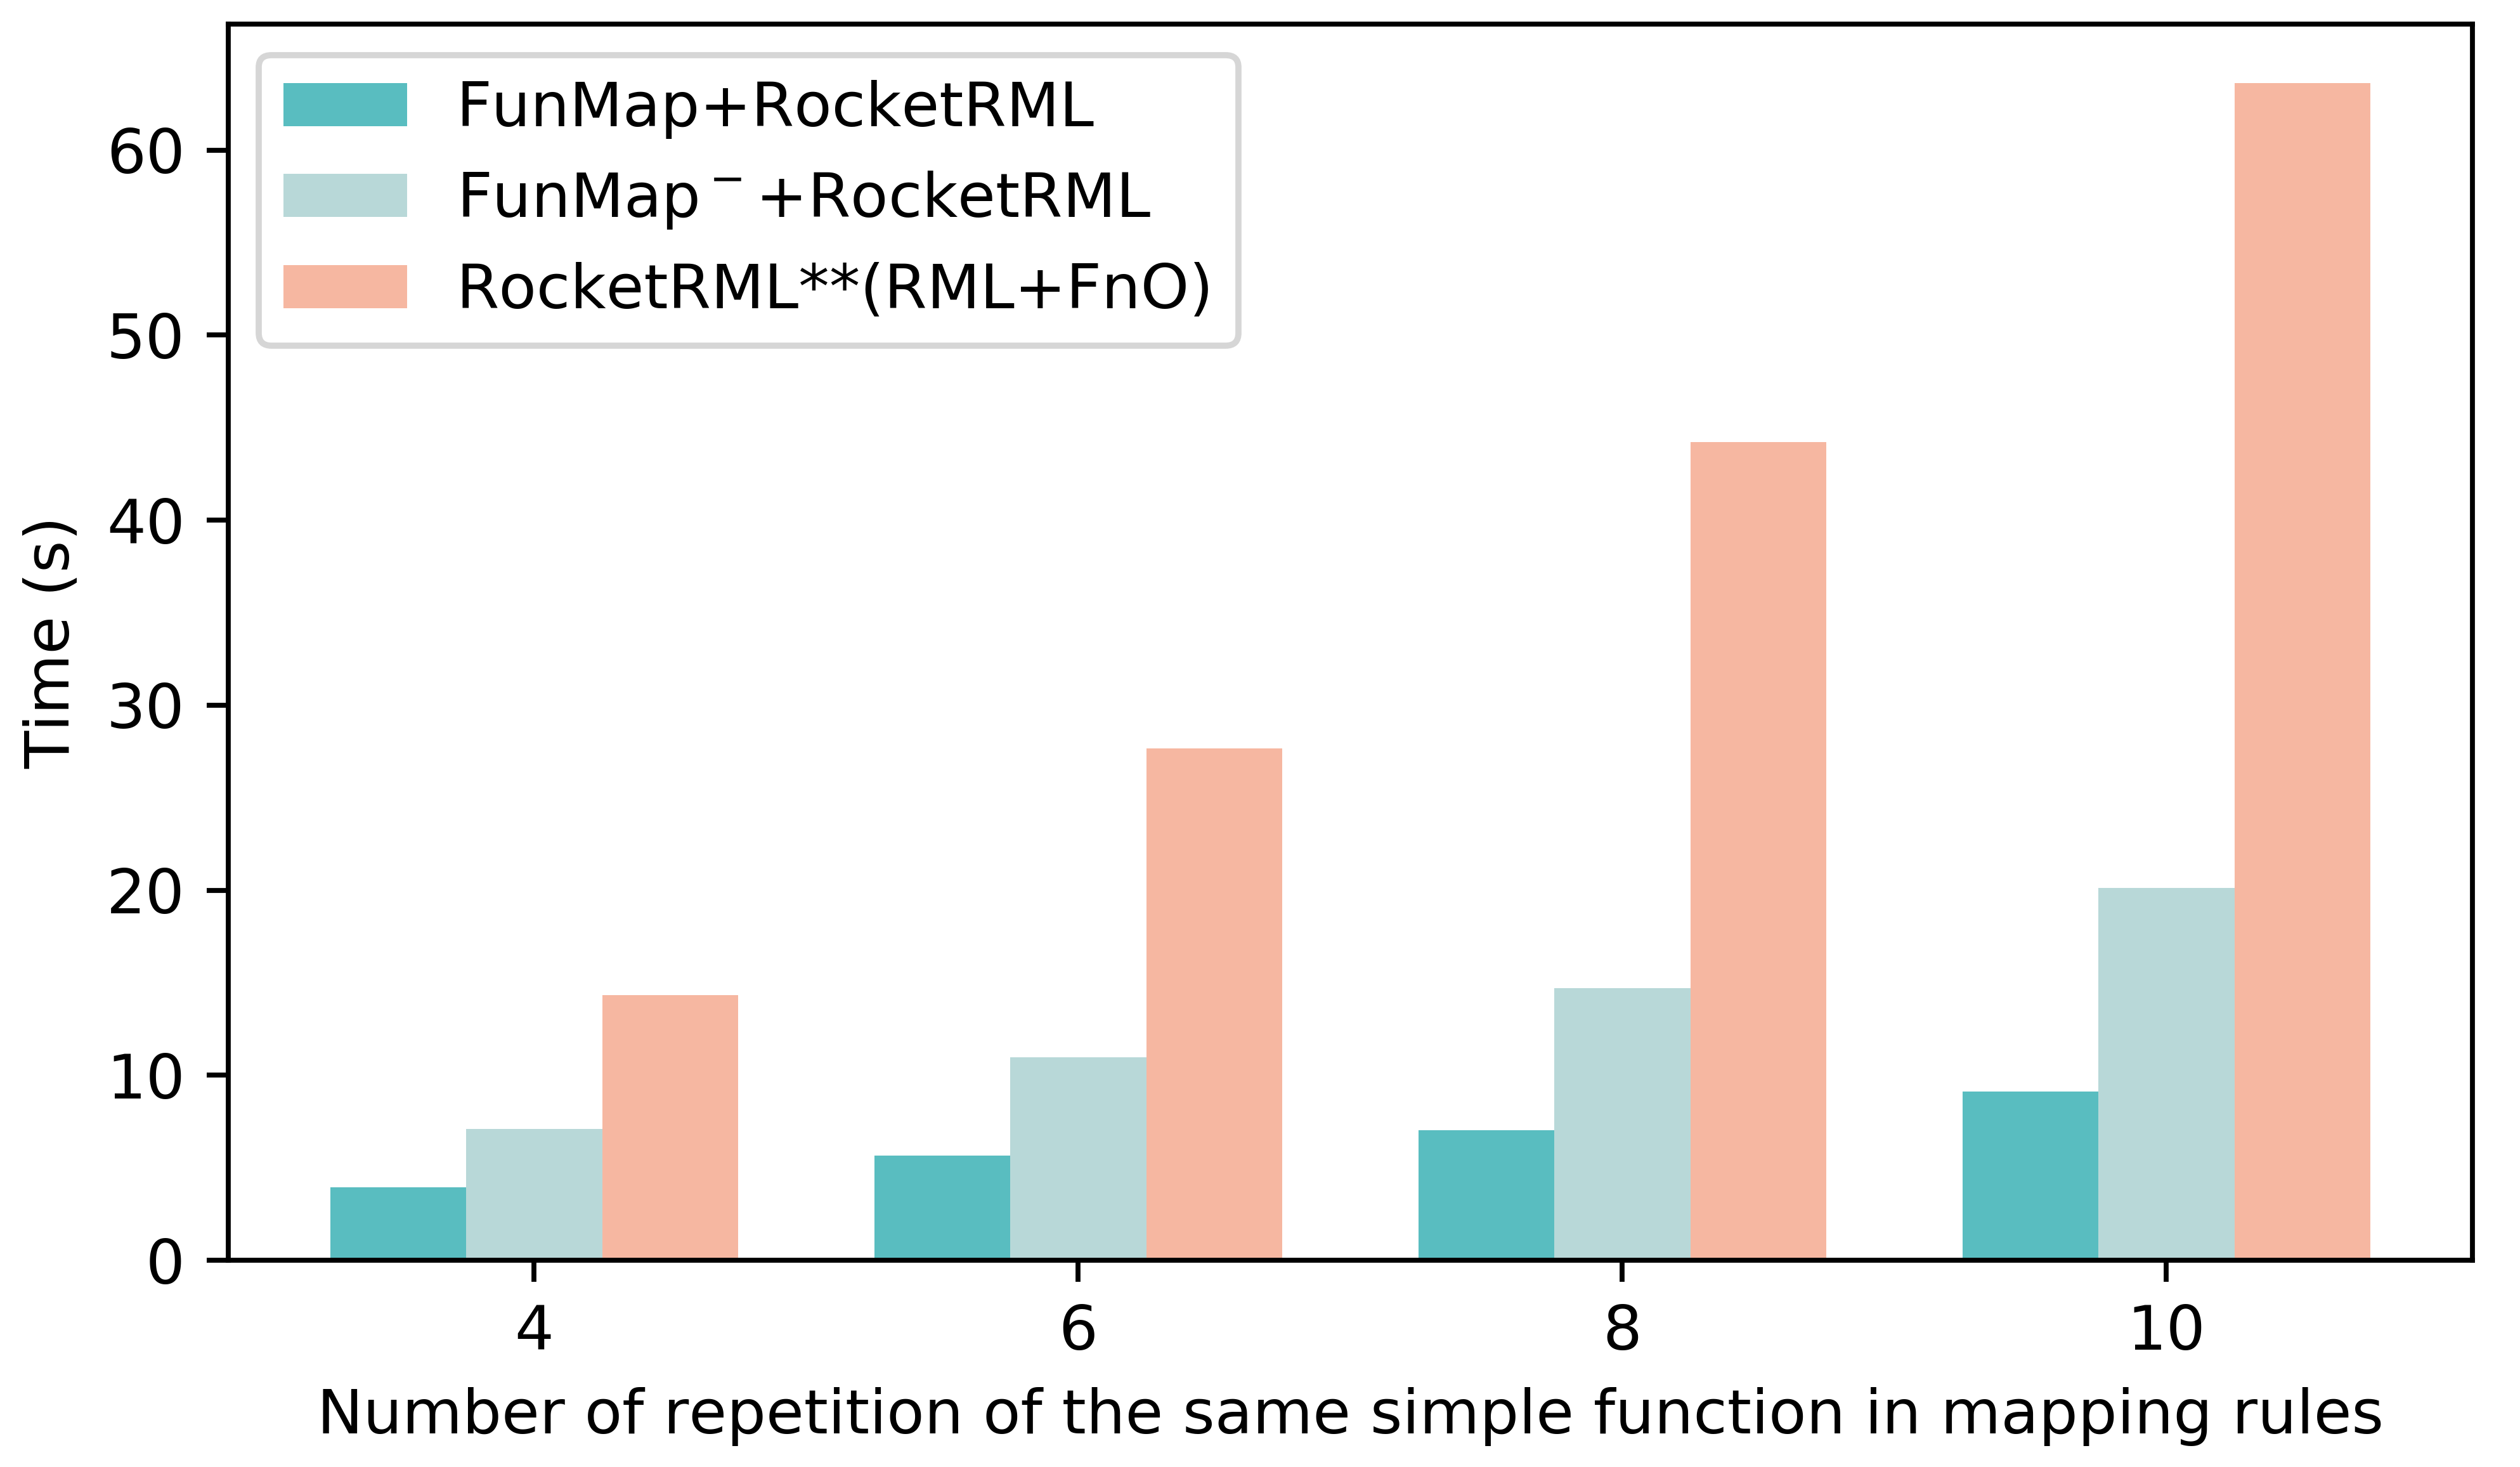
\includegraphics[width=0.45\columnwidth]{figures/veracity75_rocketrml.png}
            \label{fig:vera75_rocketrml}}
\caption[Execution time with simple functions 25-75\% of duplicates]{{\bf Total execution time of experiments with simple functions 25-75\% of duplicates.} SDM-RDFizer, RMLMapper and RocketRML executing simple functions in RML+FnO mappings and with FunMap and FunMap$^-$.}
    \label{fig:exp-simple}
\end{figure}

\subsubsection{Discussion of Observed Results}
In this section, we describe the outcomes of our experimental evaluation. Figure \ref{fig:exp-simple} reports on the execution time of the different testbeds in which the functions are considered to be ``simple'' whereas Figure \ref{fig:exp-complex} shows the experiments involving ``complex'' functions. Both figures represent the total execution time for constructing the knowledge graph applying selected engines (i.e., SDM-RDFizer, RMLMapper, and RocketRML) in three different configurations: a) the current version of the engine that is able to directly interpret RML+FnO mappings in the engine (e.g., RMLMapper**(RML+FnO)); b) FunMap$^-$ in conjunction with the engine (e.g., FunMap$^-$+RMLMapper); and c) FunMap together with the engine (e.g., FunMap+RMLMapper). In the case of all the configuration of RocketRML, we only provide the results for the execution of simple functions because the engine does not execute joins with multiple conditions correctly, hence, the proposed optimizations cannot be applied. For the rest of the experiments, we have verified that the results are the same for all the approaches in terms of cardinality and correctness. 
\begin{figure}[t!]
 \centering
    \subfloat[SDM-RDFizer - 25\% of duplicates]{
        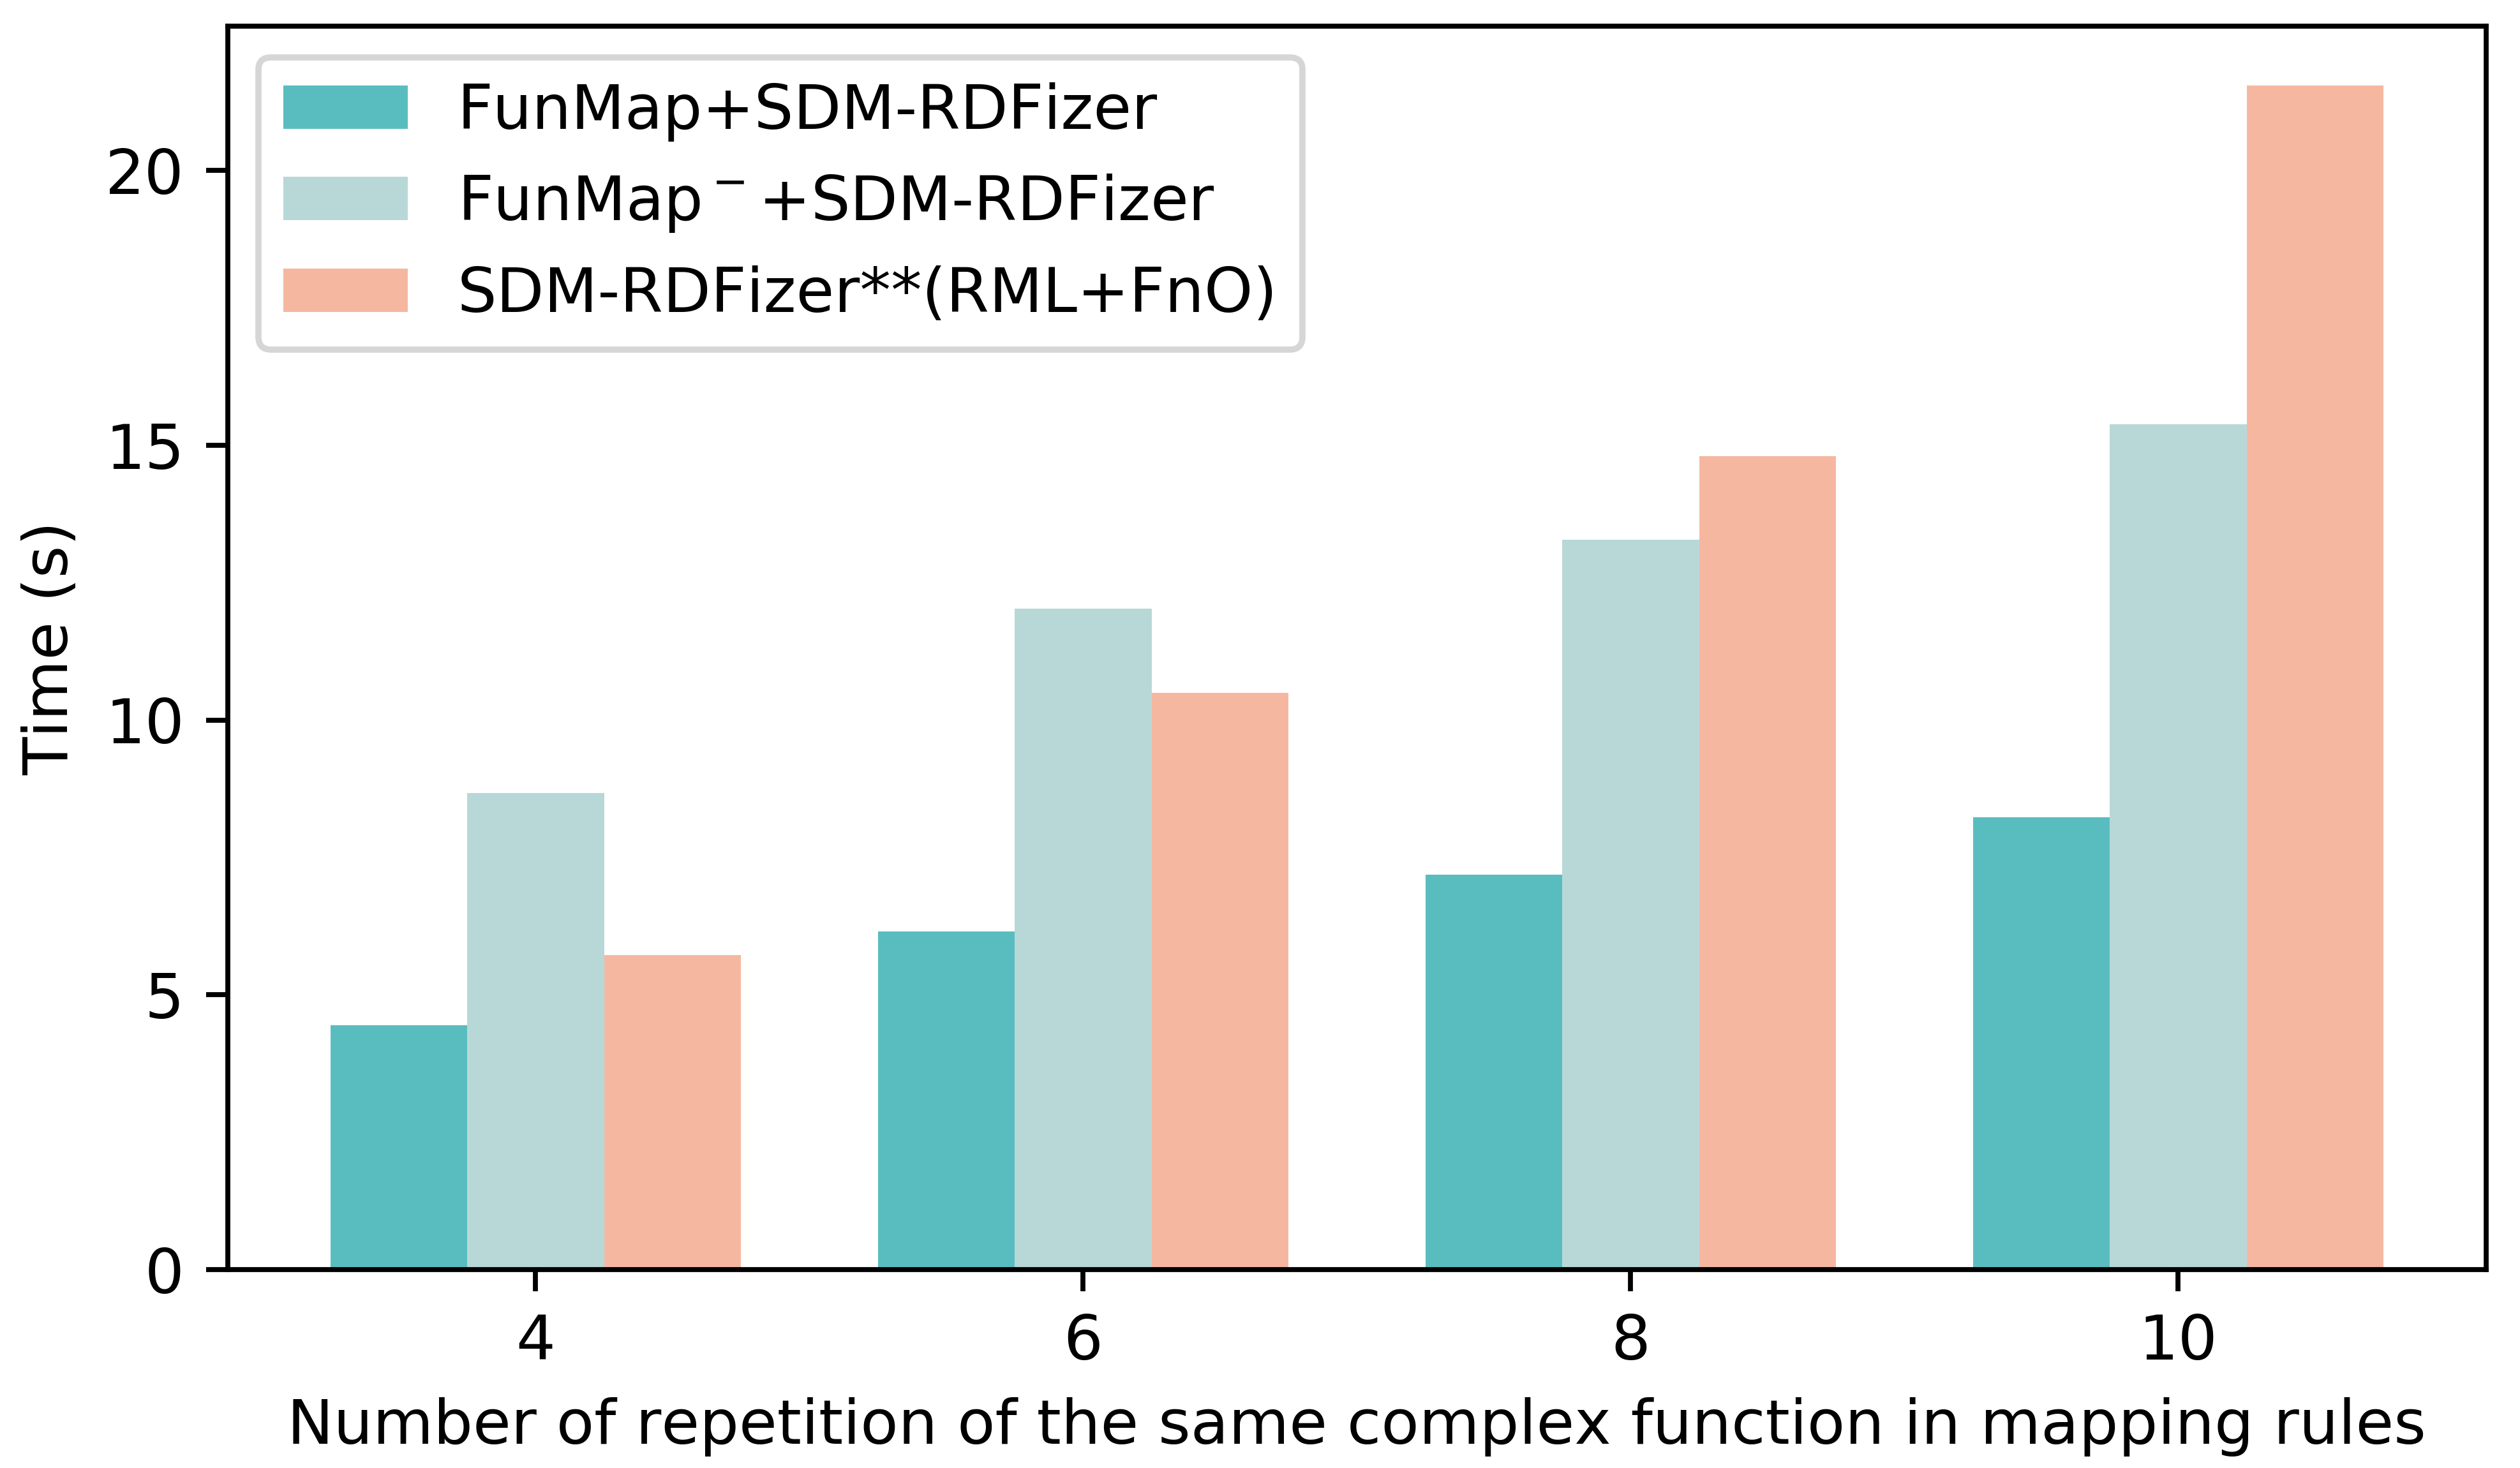
\includegraphics[width=0.45\columnwidth]{figures/veracity25_sdmrdfizer_complex.png}
            \label{fig:vera25_sdmrdfizer_mapsdi}}
    \subfloat[SDM-RDFizer - 75\% of duplicates]{
        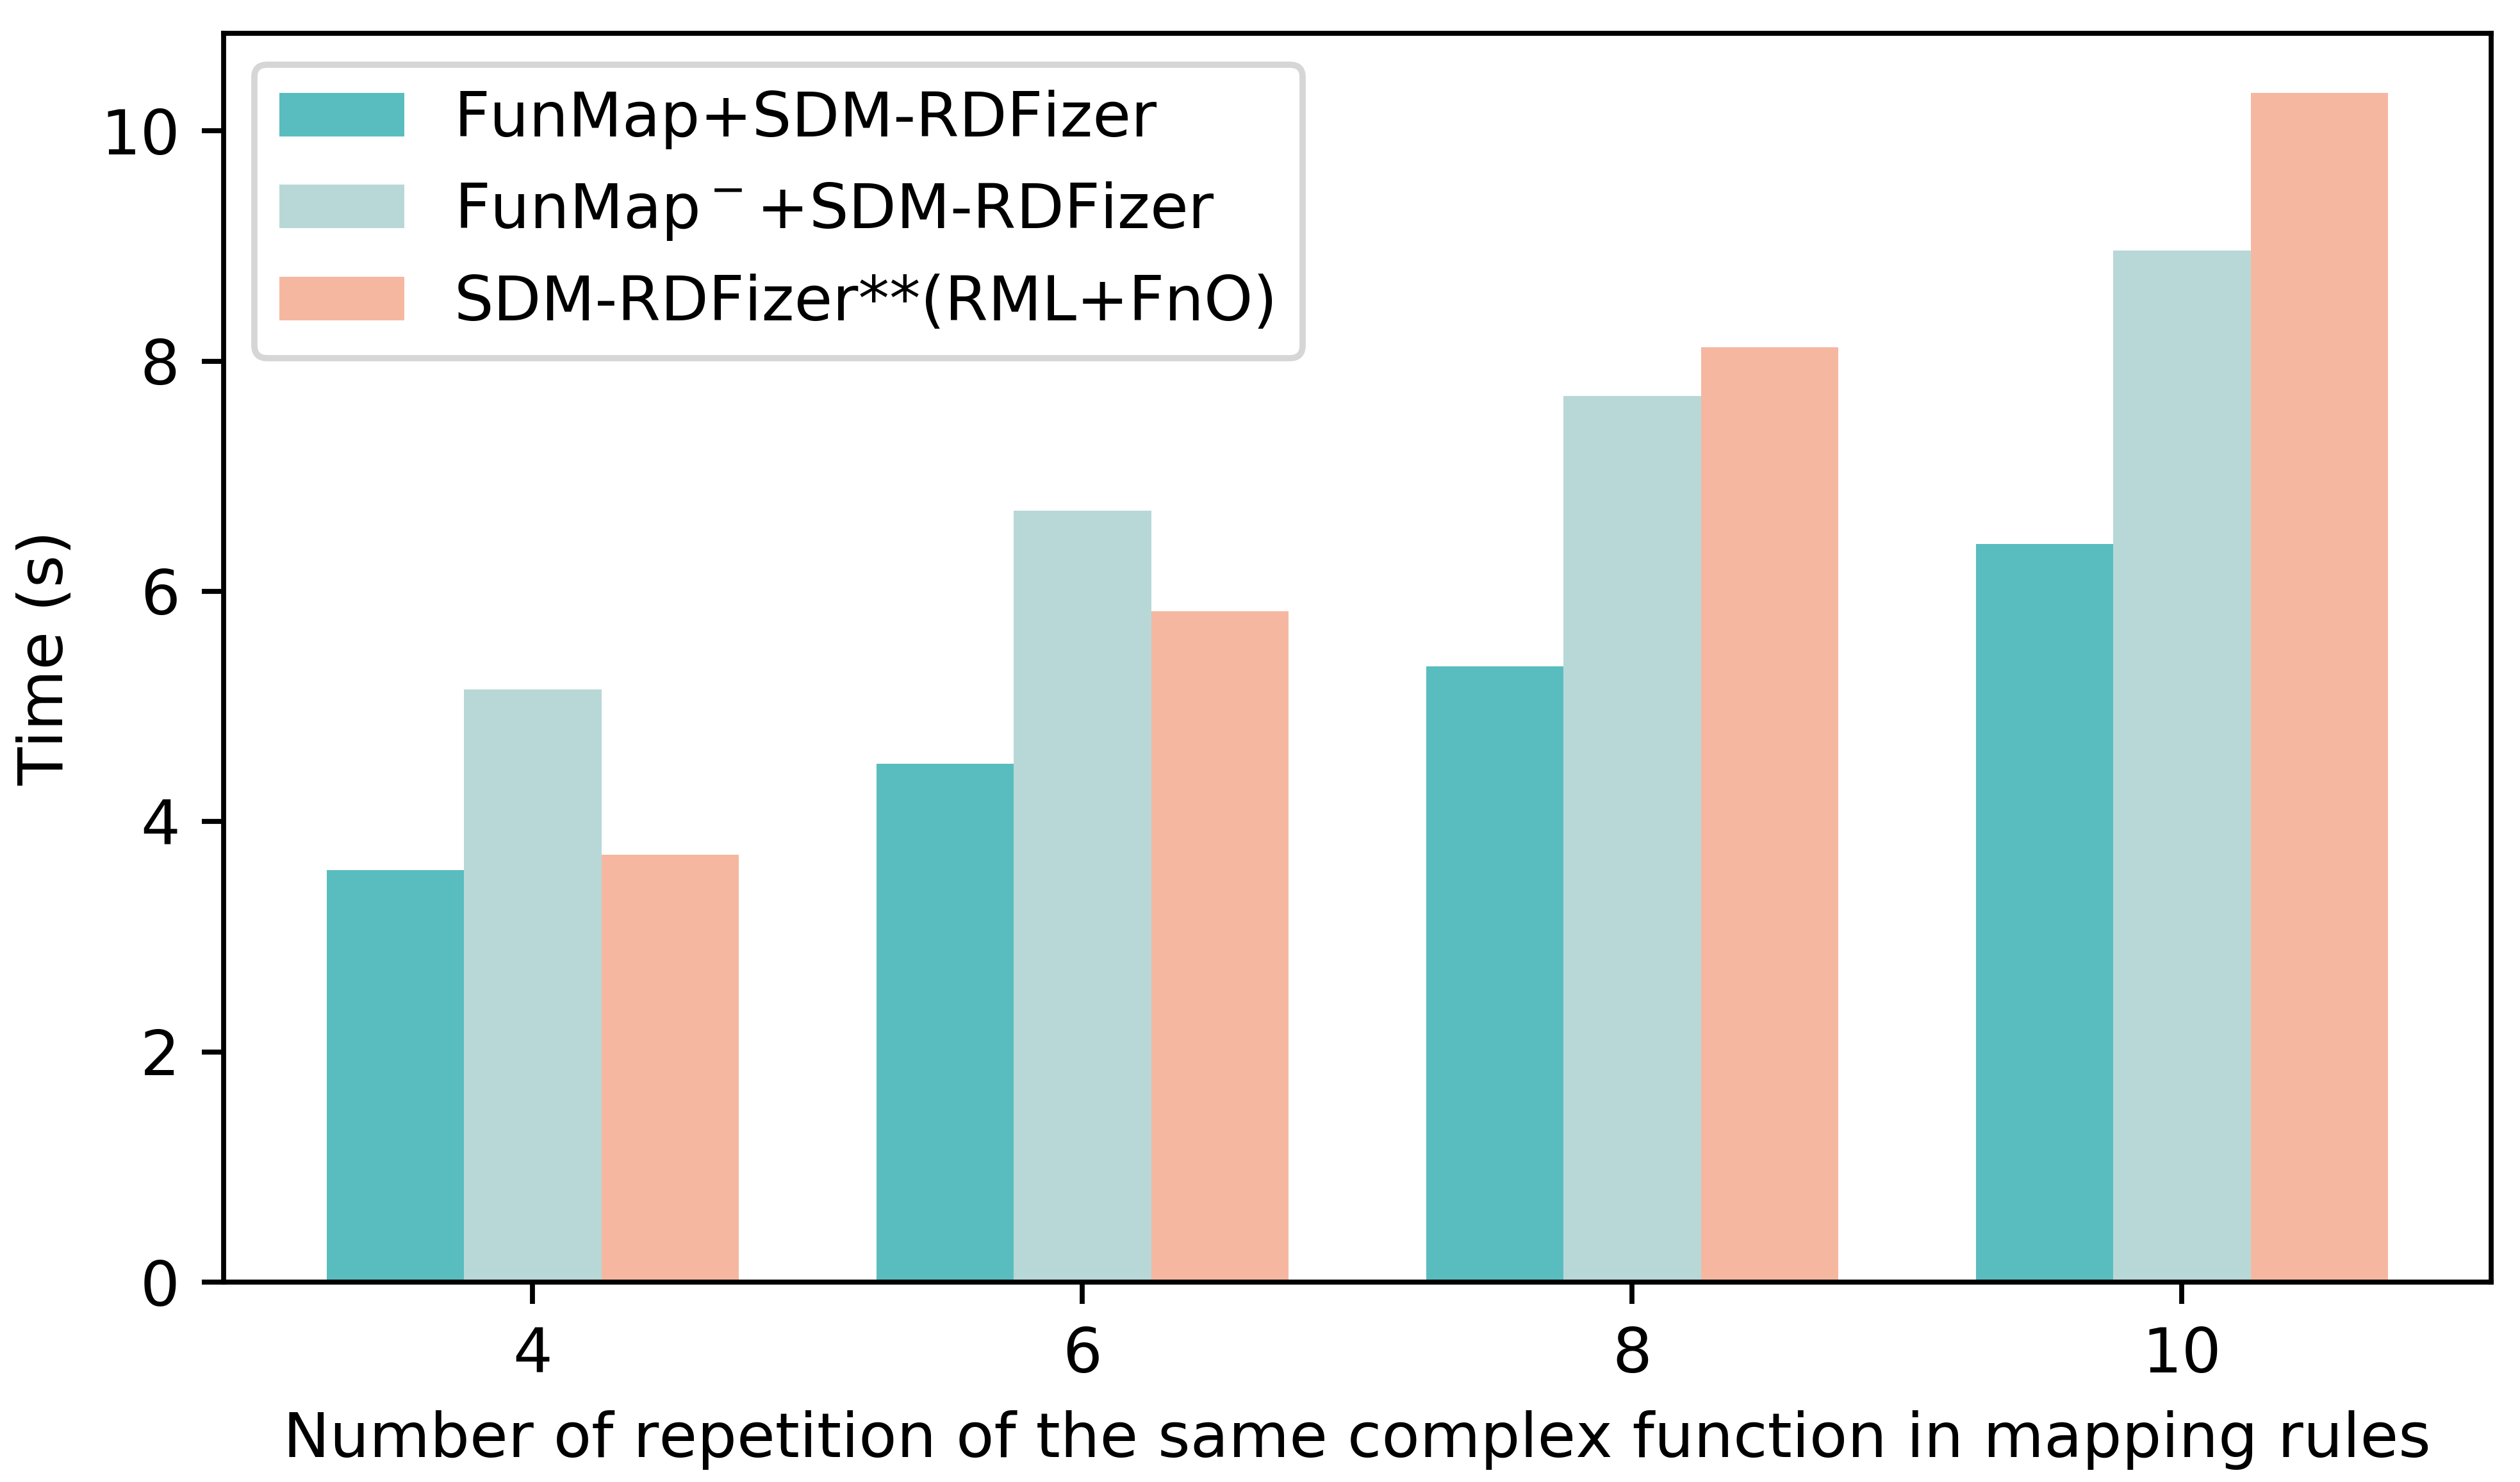
\includegraphics[width=0.45\columnwidth]{figures/veracity75_sdmrdfizer_complex.png}
            \label{fig:vera75_sdmrdfizer_MapSDI}}
\\            
    \subfloat[RMLMapper - 25\% of duplicates]{
        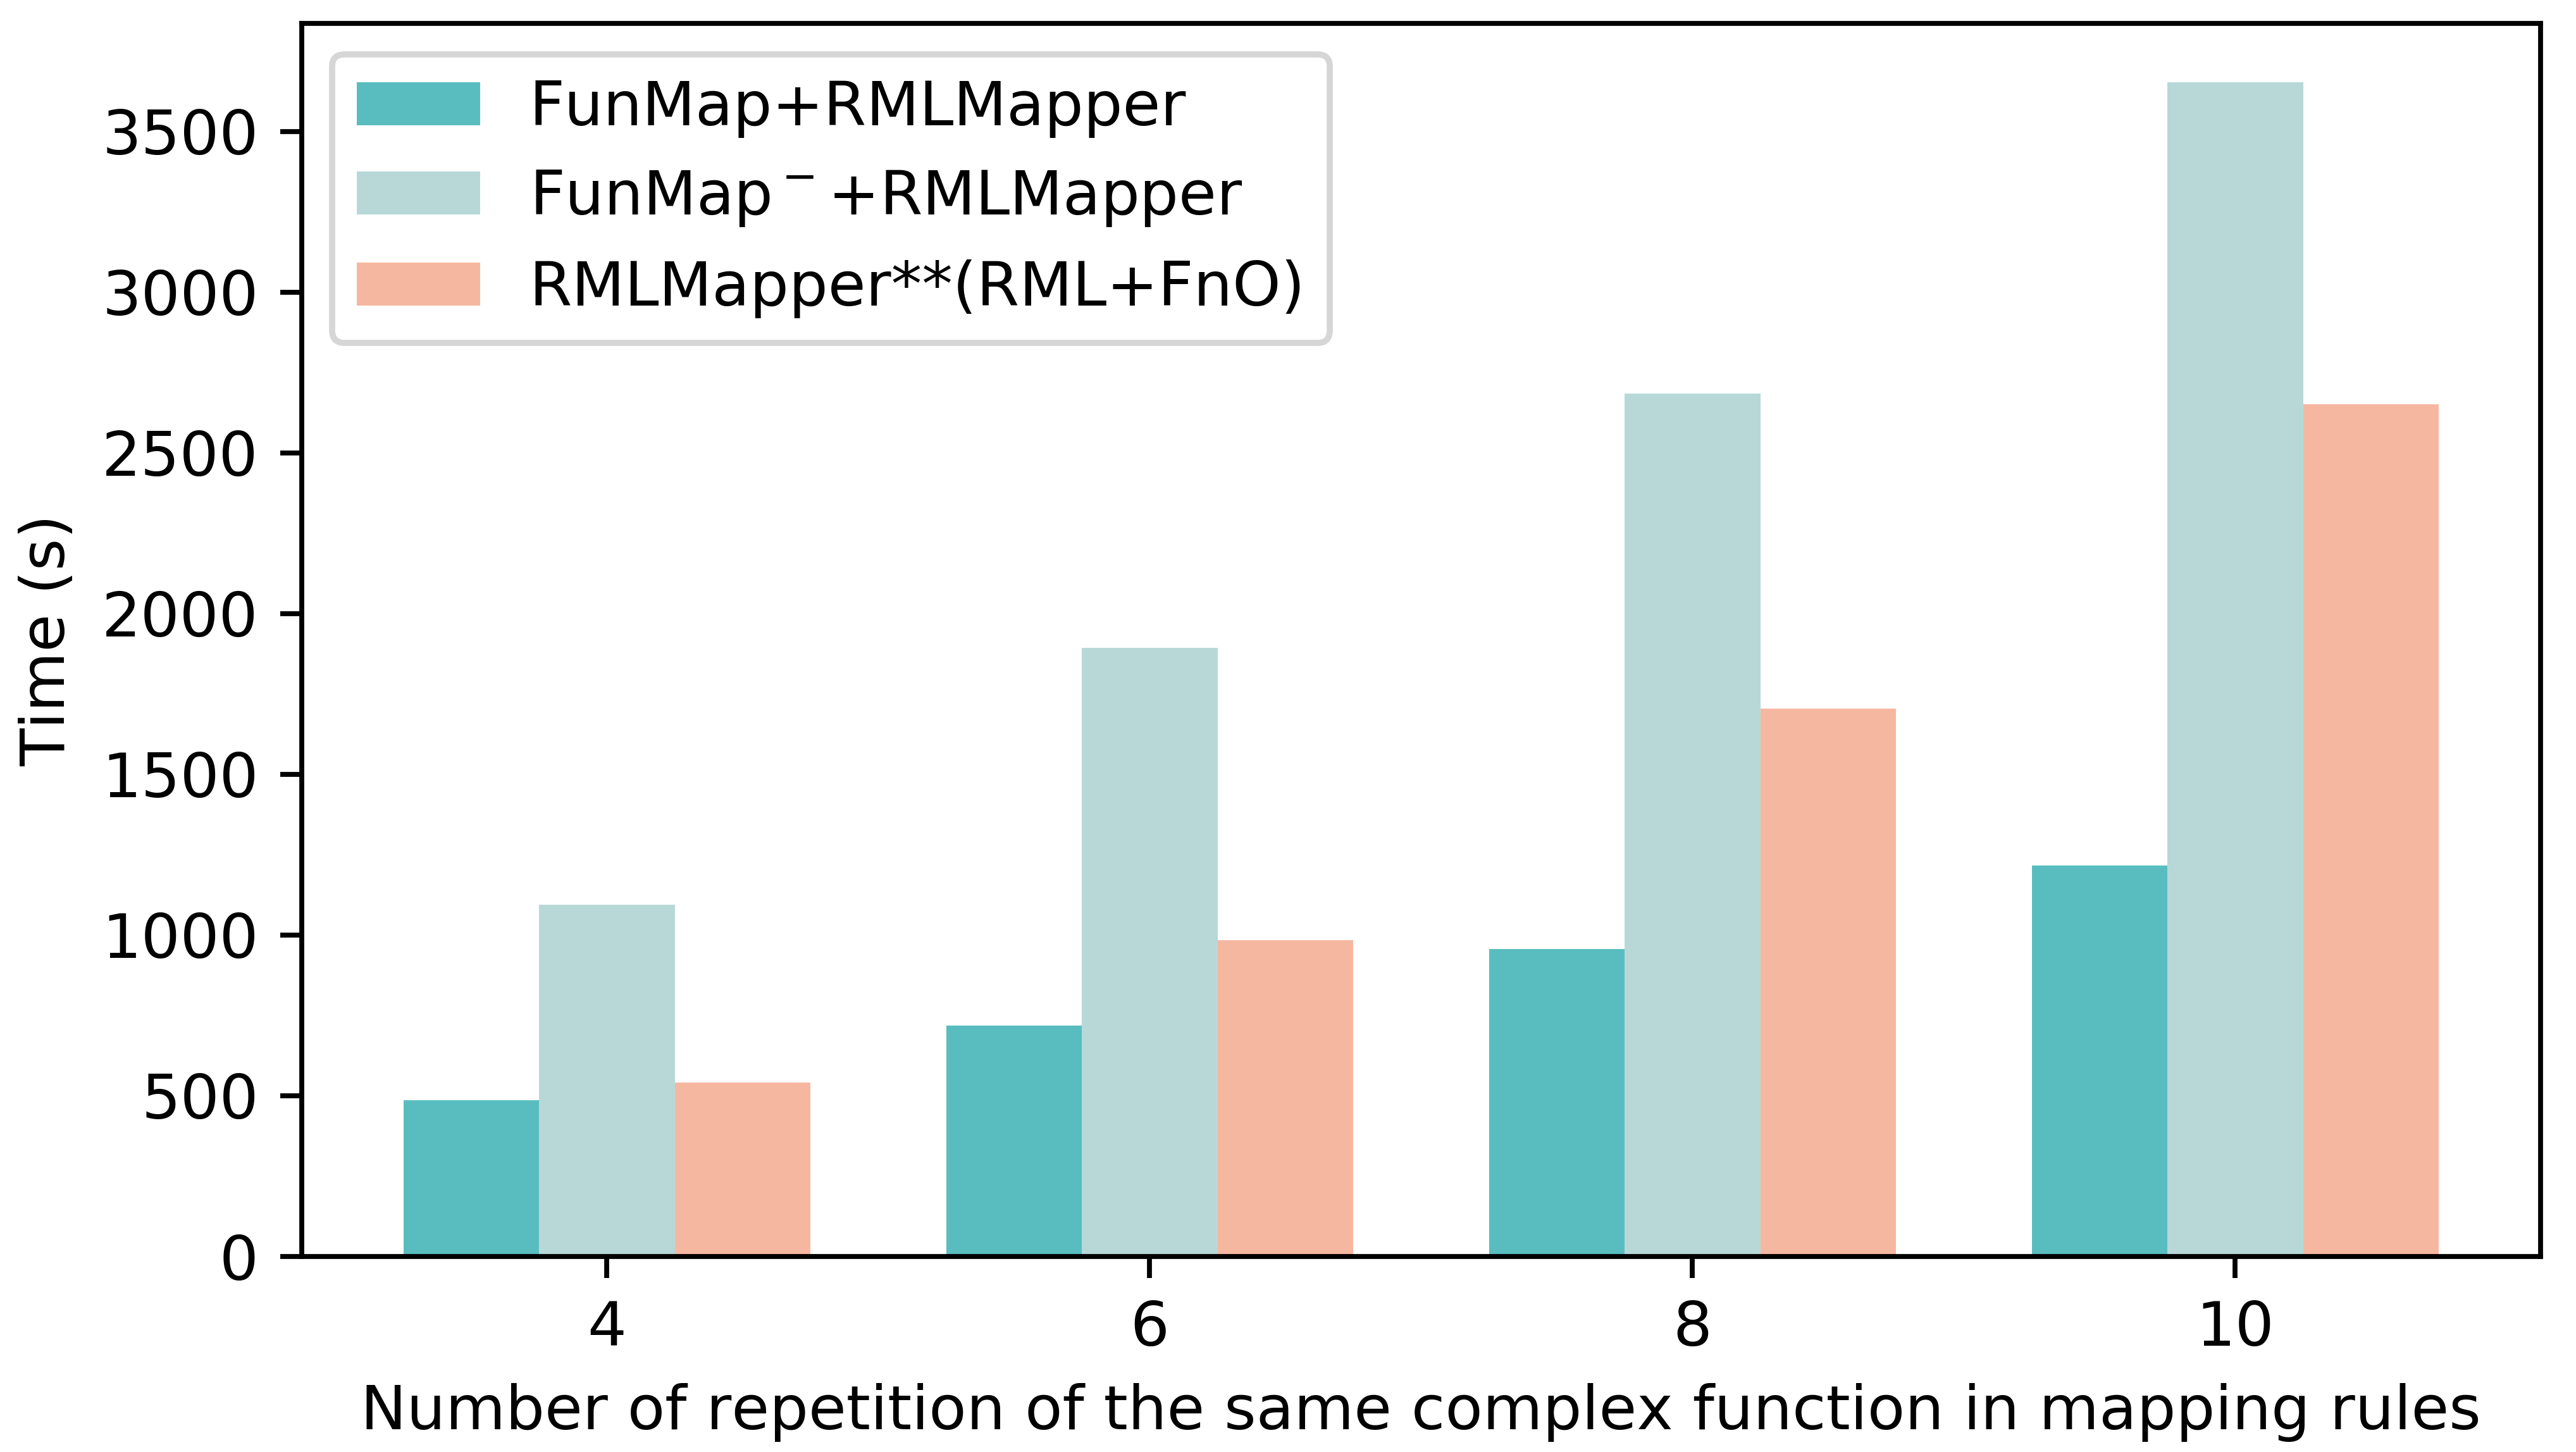
\includegraphics[width=0.45\columnwidth]{figures/veracity25_rmlmapper_complex.png}
            \label{fig:vera25_rmlmapper_MapSDI}}  
    \subfloat[RMLMapper - 75\% of duplicates]{
        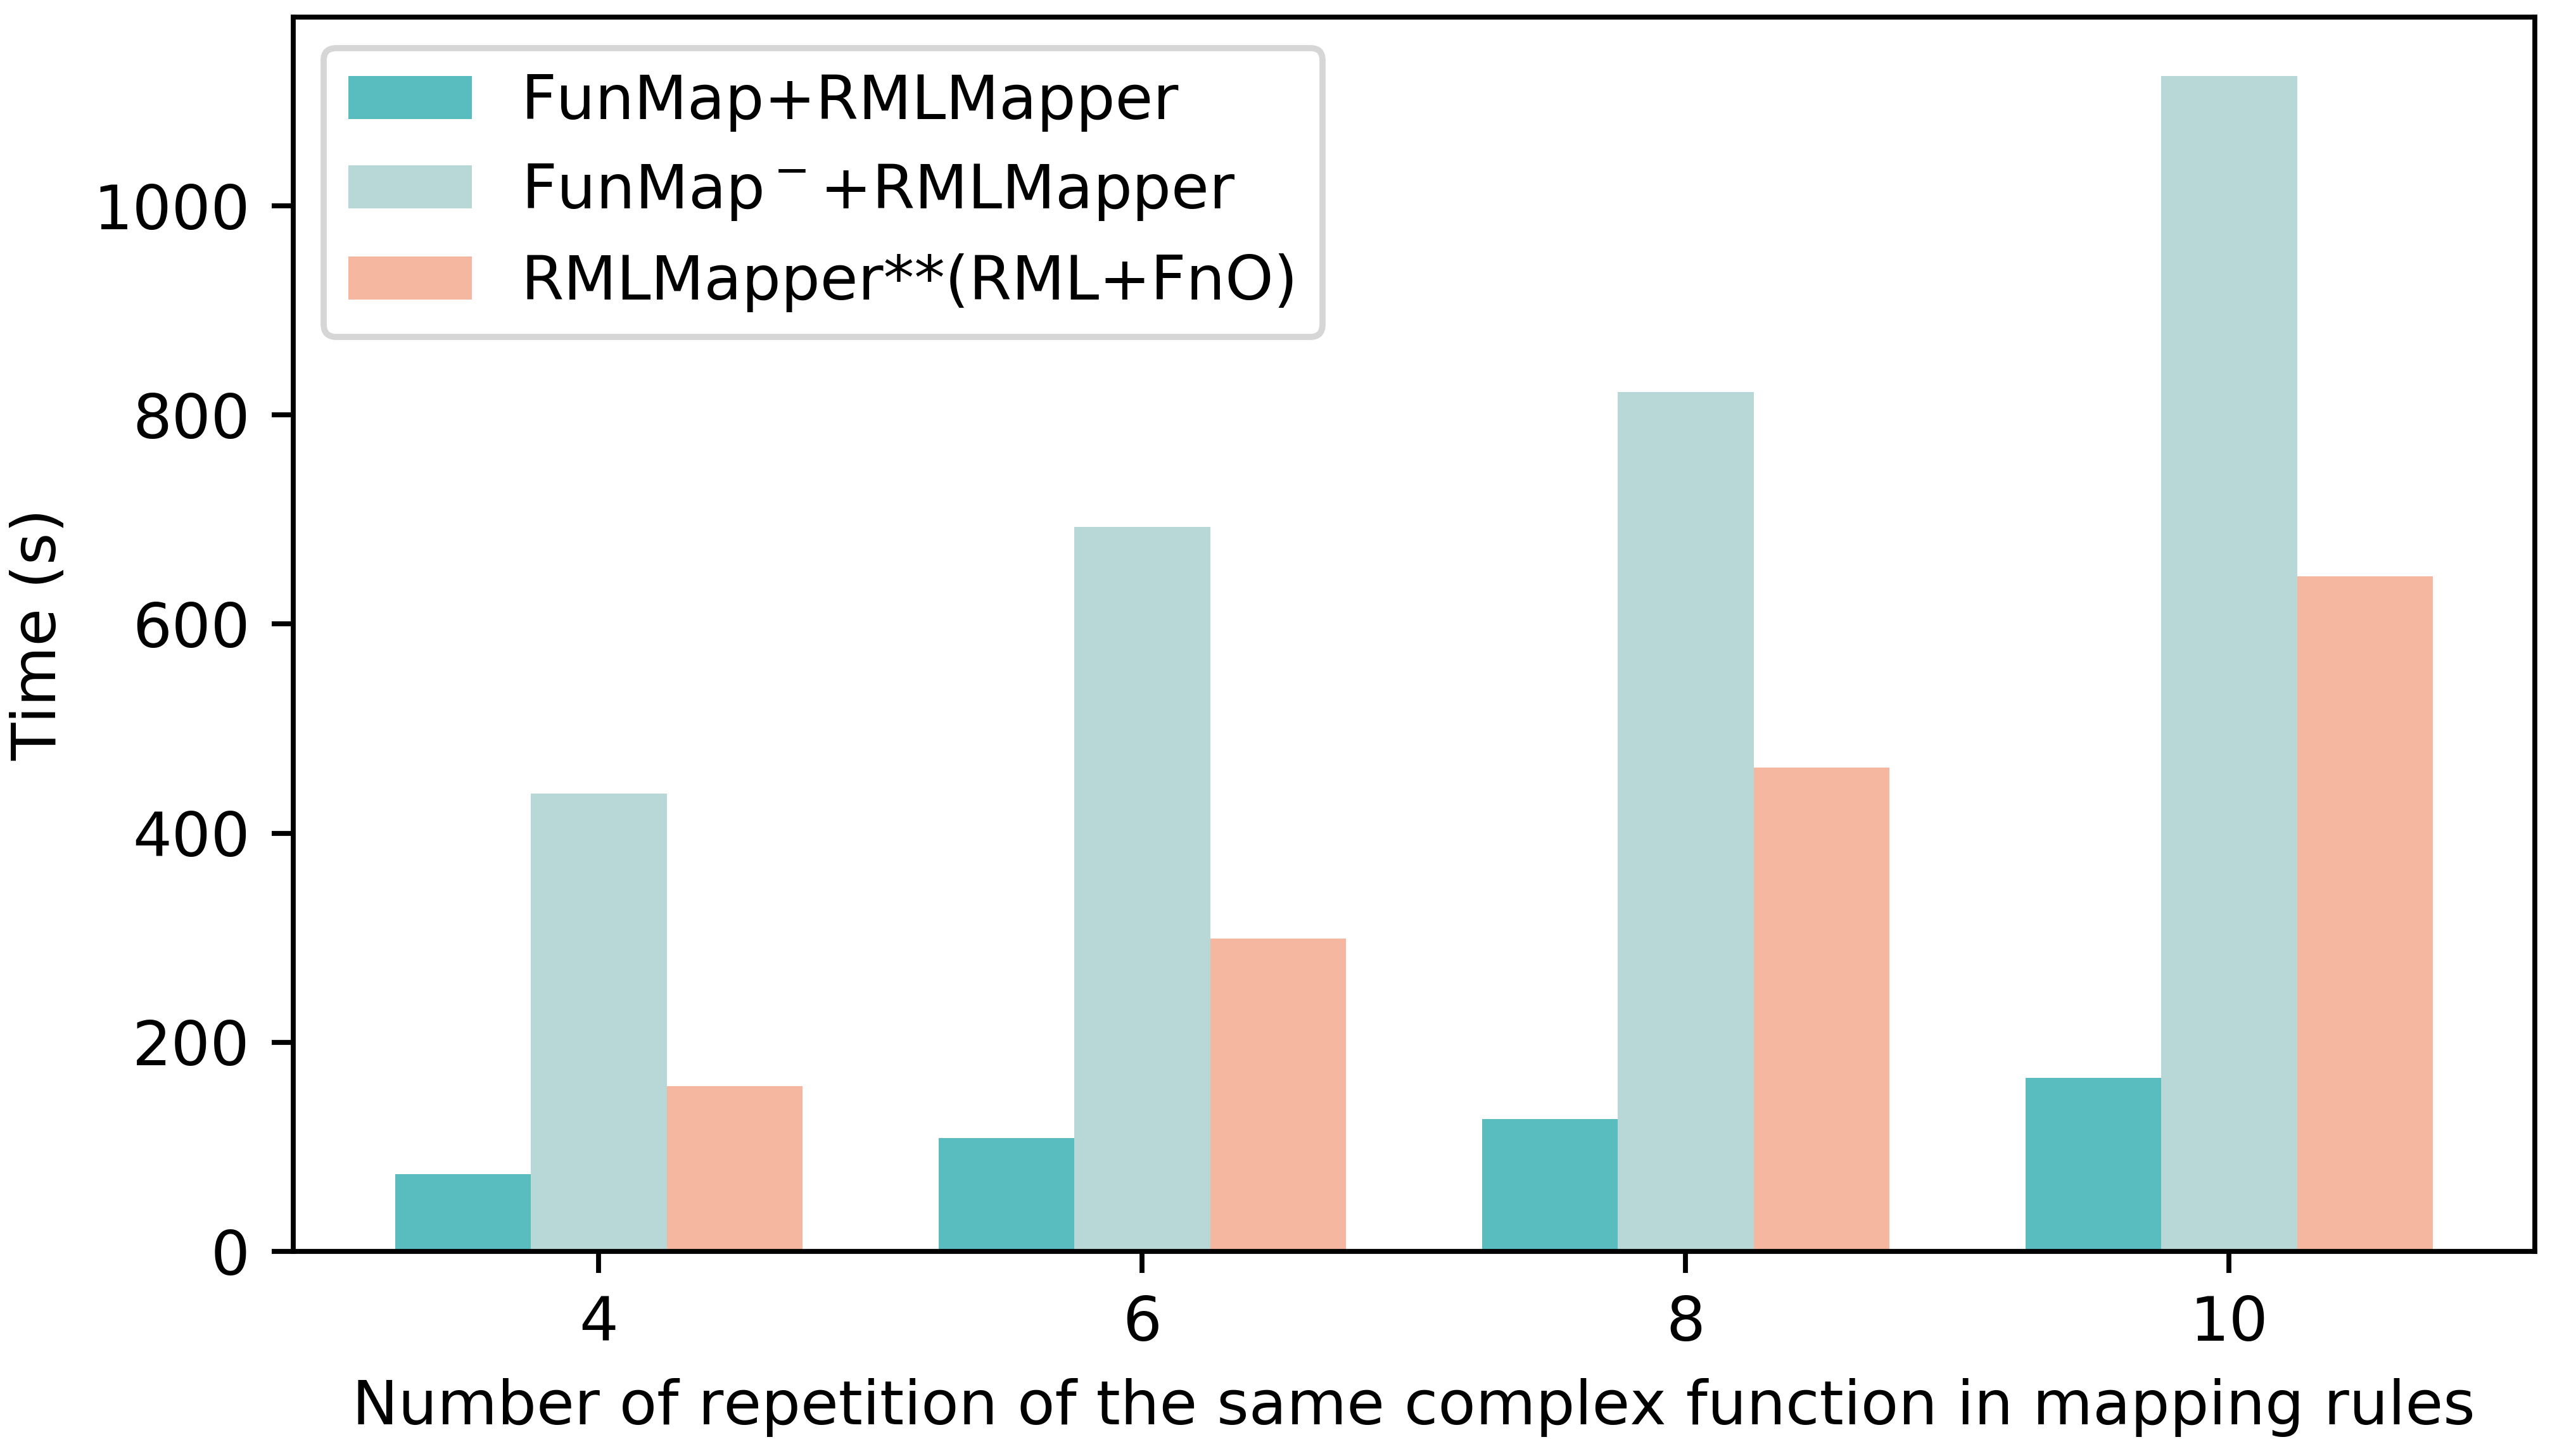
\includegraphics[width=0.45\columnwidth]{figures/veracity75_rmlmapper_complex.png}
            \label{fig:vera75_rmlmapper_MapSDI}} 
\caption[Execution time with complex functions 25-75\% of duplicates]{{\bf Total execution time for complex functions 25-75\% of duplicates.} SDM-RDFizer and RMLMapper executing complex functions in RML+FnO mappings and with FunMap and FunMap$^-$.}
    \label{fig:exp-complex}
\end{figure}

The results obtained by the application of SDM-RDFizer with the repetition of simple functions (Figures \ref{fig:vera25_sdmrdfizer} and \ref{fig:vera75_sdmrdfizer}) reflect an improvement of the execution time when FunMap is applied in the process. With the growth of number of duplicates and repeated functions, the difference between the performance of SDM-RDFizer**(RML+FnO) and FunMap+SDM-RDFizer increases. Using this engine, FunMap$^-$ shows the same behavior as FunMap, however, in the case of having a large number of duplicates and a few repeated functions FunMap$^-$ does not improve the performance of SDM-RDFizer**(RML+FnO). 
In the case of using RMLMapper (Figures \ref{fig:vera25_rmlmapper} and \ref{fig:vera75_rmlmapper}), we observe that the results obtained together with FunMap$^-$ (i.e., DTR1 optimization) do not show better performance than RMLMapper**(RML+FnO). DTR1 which only focuses on transforming functions, delegates the removal of the duplicates to the engine which is not accomplished efficiently by RMLMapper. However, in FunMap+RMLMapper, that includes DTR1 and DTR2 optimizations, duplicates are removed before the execution of the RML mappings and leads to obtain the results that clearly show improvements with respect to the baseline. In the same manner as the SDM-RDFizer, the number of repetitions of the functions affects the execution time of the RMLMapper**(RML+FnO), while FunMap maintains similar execution times. Finally, RocketRML (Figures \ref{fig:vera25_rocketrml} and \ref{fig:vera75_rocketrml}) seems not to be affected by the number of duplicates over the input data, obtaining similar execution times for 25\% and 75\% rate for RocketRML**(RML+FnO). However, the number of repetitions over functions impacts the performance of RocketRML**(RML+FnO), increasing the total execution time. The incorporation of DTR1 (i.e., FunMap$^-$+RocketRML) and DTR2 (i.e., FunMap + RocketRML) enhances the performance and scalability during the construction of the knowledge graph, obtaining a similar behavior as the other two tested engines. 

The effect of function complexity over SDM-RDFizer can be observed in Figures \ref{fig:vera25_sdmrdfizer_mapsdi} and \ref{fig:vera75_sdmrdfizer_MapSDI}. Whenever the number of repetitions is low (4-6), the join with multiple conditions affects FunMap$^-$ + SDM-RDFizer, obtaining worse results than SDM-RDFizer**(RML+FnO). However, if repetitions increase (8-10), DTR1 empowers SDM-RDFizer**(RML+FnO) due the reduction of repeated operations during the evaluation of the mappings. Conversely, FunMap together with SDM-RDFizer exhibits better results than SDM-RDFizer**(RML+FnO) in all the testbeds. Finally, the behavior of RMLMapper -- when it has to execute complex transformation functions (Figures \ref{fig:vera25_rmlmapper_MapSDI} and \ref{fig:vera75_rmlmapper_MapSDI})-- is affected in terms of execution time for the configuration FunMap$^-$+RMLMapper in comparison to the case of simple functions. As similar as SDM-RDFizer, the join with several conditions is impacting the performance. However, together with data transformation optimizations, FunMap+RMLMapper outperforms the baseline. 

The experimental results on RDBs show even more significant improvement in the performance of both RMLMapper and SDM-RDFizer in the presence of FunMap. In the case of FunMap+RMLMapper, applying \verb|join|s in the SQL queries that define the \verb|logicalSource|s instead of using \verb|joinCondition|s reduces execution time by up to a factor of 18. These results evidence that \verb|joinCondition|s are not efficiently implemented by RMLMapper, and explain why FunMap+RMLMapper is showing less improvement compared to FunMap+SDM-RDFizer in \autoref{fig:exp-complex}. Moreover, FunMap+SDM-RDFizer successfully performs on the large-sized relational dataset of 1.3GB in 5,670.67 seconds, while SDM-RDFizer**(RML+FnO) cannot create the KG and times out after 10,000 seconds.

In overall, we observe that the configurations that interpret RML+FnO mappings directly are affected by the repetition of the functions and the degree of data duplicates, i.e., execution time monotonically increases with number of functions and data duplication degree. In contrast, the incorporation of FunMap to the engines shows less fluctuated behavior when the data duplication rate increases. Additionally, the studied engines handle the repetition of the functions during the construction of the knowledge graph thanks to the pushing down of the execution of the functions directly over the dataset.
In summary, the observed results indicate that the FunMap heuristics improve the performance of data integration systems and generate solutions to the problem of scaled-up knowledge graph construction. The effectiveness of the proposed transformations has been empirically demonstrated on various RML+FnO and RML-compliant engines. However, we observe that there are cases where the application of DTR1 alone is not enough (i.e., FunMap$^-$), being required the applications of all the transformations (i.e., DTRs and MTRs) to provide an effective solution. 


\subsection{Conclusions}

In this section, we addressed the problem of scaled-up KG construction in complex data integration systems, i.e., systems with large data sources, high data duplication rate, and functional mappings. We presented a heuristic-based approach for efficiently evaluating data integration systems with data sources in diverse formats (e.g., CSV or relational). The proposed heuristics are implemented in FunMap, an interpreter of RML+FnO, that converts data integration systems in RML+FnO into equivalent data integration systems specified in RML. Besides shaping an RML-engine independent interpreter of RML+FnO, FunMap generates data integration systems that enhance RML-compliant engines whenever transformation functions are repeatedly used, and data sources are large and have highly-duplicated data. Empirical evaluations of the combination of FunMap with RML-compliant engines suggest that the execution time of RML+FnO can be reduced by up to a factor of 18. Thus, FunMap widens the repertory of tools to scale up knowledge graphs to the enormous increase of incoming data and ease the development of real-world KG applications. As the main limitation, FunMap can only be applied with an RML-compliant engine which supports either \verb|joinCondition| or RDB on the backend. We plan to devise cost-based optimization approaches that, together with the proposed heuristics, allow for the generation of the best solution for a complex data integration system in RML+FnO. 


\section{Conclusions on materialized KGC at scale}